% !Mode:: "TeX:UTF-8"

\def\usewhat{xelatex}                               % 定义编译方式 dvipdfmx 或者 pdflatex，默认为 dvipdfmx
                                                     % 方式编译，如果需要修改，只需改变花括号中的内容即可。
\documentclass[12pt,openany,oneside,ctexartutf8]{book}
                                                     % 本科生毕业论文通常采用单页排版
\input{setup/package}                                % 定义本文所使用宏包
\graphicspath{{figures/}{images/}}                   % 图片搜索路径：figures/（封面Logo）和 images/（正文插图）
\begin{document}                                     % 开始全文
\def\atemp{pdflatex}\ifx\atemp\usewhat
\begin{CJK*}{UTF8}{song}                             % 开始中文字体使用（仅 pdflatex 模式）
\fi
	% !Mode:: "TeX:UTF-8"
%  Authors: 张井   Jing Zhang: prayever@gmail.com     天津大学2010级管理与经济学部信息管理与信息系统专业硕士生
%           余蓝涛 Lantao Yu: lantaoyu1991@gmail.com  天津大学2008级精密仪器与光电子工程学院测控技术与仪器专业本科生

% 2018/5/23修正
%           李幼萌 Youmeng Li: liyoumeng@tju.edu.cn   天津大学软件学院软件工程系

%%%%%%%%%%%%%%%%% Fonts Definition and Basics %%%%%%%%%%%%%%%%%
% 根据编译方式定义字体命令
\def\atemp{xelatex}\ifx\atemp\usewhat
% xelatex 模式：使用 ctex 的字体定义（避免依赖 macOS 系统字体）
\newcommand{\song}{\songti}             % 宋体
\newcommand{\fs}{\fangsong}             % 仿宋体
\newcommand{\kai}{\kaishu}              % 楷体
\newcommand{\hei}{\heiti}               % 黑体
\newcommand{\li}{\lishu}                % 隶书
\else
% pdflatex 模式：使用原有的 CJK 字体定义
\newcommand{\song}{\CJKfamily{song}}    % 宋体
\newcommand{\fs}{\CJKfamily{fs}}        % 仿宋体
\newcommand{\kai}{\CJKfamily{kai}}      % 楷体
\newcommand{\hei}{\CJKfamily{hei}}      % 黑体
\newcommand{\li}{\CJKfamily{li}}        % 隶书
\fi
\newcommand{\yihao}{\fontsize{26pt}{26pt}\selectfont}       % 一号, 单倍行距
\newcommand{\xiaoyi}{\fontsize{24pt}{24pt}\selectfont}      % 小一, 单倍行距
\newcommand{\erhao}{\fontsize{22pt}{1.25\baselineskip}\selectfont}       % 二号, 1.25倍行距
\newcommand{\xiaoer}{\fontsize{18pt}{18pt}\selectfont}      % 小二, 单倍行距
\newcommand{\sanhao}{\fontsize{16pt}{16pt}\selectfont}      % 三号, 单倍行距
\newcommand{\xiaosan}{\fontsize{15pt}{15pt}\selectfont}     % 小三, 单倍行距
\newcommand{\sihao}{\fontsize{14pt}{14pt}\selectfont}       % 四号, 单倍行距
\newcommand{\xiaosi}{\fontsize{12pt}{12pt}\selectfont}      % 小四, 单倍行距
\newcommand{\wuhao}{\fontsize{10.5pt}{10.5pt}\selectfont}   % 五号, 单倍行距
\newcommand{\xiaowu}{\fontsize{9pt}{9pt}\selectfont}        % 小五, 单倍行距

% 根据编译方式处理 CJK 相关命令
\def\atemp{pdflatex}\ifx\atemp\usewhat
\CJKtilde  % 重新定义了波浪符~的意义（仅 pdflatex 模式）
\fi
\newcommand\prechaptername{第}
\newcommand\postchaptername{章}

% 根据编译方式处理标点符号
\def\atemp{pdflatex}\ifx\atemp\usewhat
\punctstyle{hangmobanjiao}             % 调整中文字符的表示，行内占一个字符宽度，行尾占半个字符宽度（仅 pdflatex 模式）
\fi

% 调整罗列环境的布局
\setitemize{leftmargin=3em,itemsep=0em,partopsep=0em,parsep=0em,topsep=-0em}
\setenumerate{leftmargin=3em,itemsep=0em,partopsep=0em,parsep=0em,topsep=0em}

% 避免宏包 hyperref 和 arydshln 不兼容带来的目录链接失效的问题。
\def\temp{\relax}
\let\temp\addcontentsline
\gdef\addcontentsline{\phantomsection\temp}

% 自定义项目列表标签及格式 \begin{publist} 列表项 \end{publist}
\newcounter{pubctr} %自定义新计数器
\newenvironment{publist}{%%%%%定义新环境
\begin{list}{[\arabic{pubctr}]} %%标签格式
    {
     \usecounter{pubctr}
     \setlength{\leftmargin}{2.5em}   % 左边界 \leftmargin =\itemindent + \labelwidth + \labelsep
     \setlength{\itemindent}{0em}     % 标号缩进量
     \setlength{\labelsep}{1em}       % 标号和列表项之间的距离,默认0.5em
     \setlength{\rightmargin}{0em}    % 右边界
     \setlength{\topsep}{0ex}         % 列表到上下文的垂直距离
     \setlength{\parsep}{0ex}         % 段落间距
     \setlength{\itemsep}{0ex}        % 标签间距
     \setlength{\listparindent}{0pt}  % 段落缩进量
    }}
{\end{list}}

\makeatletter
\renewcommand\normalsize{
  \@setfontsize\normalsize{12pt}{12pt} % 小四对应 12 pt
  \setlength\abovedisplayskip{4pt}
  \setlength\abovedisplayshortskip{4pt}
  \setlength\belowdisplayskip{\abovedisplayskip}
  \setlength\belowdisplayshortskip{\abovedisplayshortskip}
  \let\@listi\@listI}
\def\defaultfont{\renewcommand{\baselinestretch}{1.63}\normalsize\selectfont} % 设置行距

% 根据编译方式控制字间距
\def\atemp{pdflatex}\ifx\atemp\usewhat
\renewcommand{\CJKglue}{\hskip -0.1 pt plus 0.08\baselineskip} % 控制字间距，使每行 34 个汉字（仅 pdflatex 模式）
\else
% xelatex 模式下使用 xeCJK 的字间距控制（如果需要）
\XeTeXlinebreaklocale "zh"
\XeTeXlinebreakskip = 0pt plus 1pt
\fi
\makeatother

%%%%%%%%%%%%% Contents %%%%%%%%%%%%%%%%%
\renewcommand{\contentsname}{目\qquad 录}
\setcounter{tocdepth}{1} % 控制目录深度
\titlecontents{chapter}[2em]{\vspace{.5\baselineskip}\xiaosan\song}
             {\prechaptername\CJKnumber{\thecontentslabel}\postchaptername\qquad}{}
             {\hspace{.5em}\titlerule*[10pt]{$\cdot$}\sihao\contentspage}
\titlecontents{section}[4.2em]{\vspace{.25\baselineskip}\sihao\song}
             {\thecontentslabel\quad}{}
             {\hspace{.5em}\titlerule*[10pt]{$\cdot$}\sihao\contentspage}
% \titlecontents{subsection}[4em]{\vspace{.25\baselineskip}\xiaosi\song}
%              {\thecontentslabel\quad}{}
%              {\hspace{.5em}\titlerule*[10pt]{$\cdot$}\sihao\contentspage}

%%%%%%%%%% Chapter and Section %%%%%%%%%%%%%
\setcounter{secnumdepth}{4}
\setlength{\parindent}{2em}

\renewcommand{\chaptername}{\prechaptername\CJKnumber{\thechapter}\postchaptername}
\titleformat{\chapter}{\centering}{\xiaosan\song}{\chaptername}{} %{2em}
\titlespacing{\chapter}{0pt}{0.1\baselineskip}{0.8\baselineskip}

\titleformat{\section}{\sihao\hei}{\thesection}{1em}{}
\titlespacing{\section}{0pt}{0.15\baselineskip}{0.25\baselineskip}

\titleformat{\subsection}{\sihao\hei}{\thesubsection}{1em}{}
\titlespacing{\subsection}{0pt}{0.1\baselineskip}{0.3\baselineskip}

\titleformat{\subsubsection}{\sihao\hei}{\thesubsubsection}{1em}{}
\titlespacing{\subsubsection}{0pt}{0.05\baselineskip}{0.1\baselineskip}

%%%%%%%%%% Table, Figure and Equation %%%%%%%%%%%%%%%%%
\renewcommand{\tablename}{表}                                     % 插表题头
\renewcommand{\figurename}{图}                                    % 插图题头
\renewcommand{\thefigure}{\arabic{chapter}-\arabic{figure}}       % 使图编号为 7-1 的格式 %\protect{~}
\renewcommand{\thesubfigure}{\alph{subfigure})}                   % 使子图编号为 a) 的格式
\renewcommand{\thesubtable}{(\alph{subtable})}                    % 使子表编号为 (a) 的格式
\renewcommand{\thetable}{\arabic{chapter}-\arabic{table}}         % 使表编号为 7-1 的格式
\renewcommand{\theequation}{\arabic{chapter}-\arabic{equation}}   % 使公式编号为 7-1 的格式

%%%%%% 定制浮动图形和表格标题样式 %%%%%%
\makeatletter
\long\def\@makecaption#1#2{
   \vskip\abovecaptionskip
   \sbox\@tempboxa{\centering\wuhao\song{#1\qquad #2} }
   \ifdim \wd\@tempboxa >\hsize
     \centering\wuhao\song{#1\qquad #2} \par
   \else
     \global \@minipagefalse
     \hb@xt@\hsize{\hfil\box\@tempboxa\hfil}
   \fi
   \vskip\belowcaptionskip}
\makeatother
\captiondelim{~~~~} %用来控制longtable表头分隔符

%%%%%%%%%% Theorem Environment %%%%%%%%%%%%%%%%%
\theoremstyle{plain}
\theorembodyfont{\song\rmfamily}
\theoremheaderfont{\hei\rmfamily}
\newtheorem{theorem}{定理~}[chapter]
\newtheorem{lemma}{引理~}[chapter]
\newtheorem{axiom}{公理~}[chapter]
\newtheorem{proposition}{命题~}[chapter]
\newtheorem{prop}{性质~}[chapter]
\newtheorem{corollary}{推论~}[chapter]
\newtheorem{definition}{定义~}[chapter]
\newtheorem{conjecture}{猜想~}[chapter]
\newtheorem{example}{例~}[chapter]
\newtheorem{remark}{注~}[chapter]
%\newtheorem{algorithm}{算法~}[chapter]
\newenvironment{proof}{\noindent{\hei 证明：}}{\hfill $ \square $ \vskip 4mm}
\theoremsymbol{$\square$}

%%%%%%%%%% Page: number, header and footer  %%%%%%%%%%%%%%%%%

%\frontmatter 或 \pagenumbering{roman}
%\mainmatter 或 \pagenumbering{arabic}
\makeatletter
\renewcommand\frontmatter{\clearpage
  \@mainmatterfalse
  }
\makeatother

%%%%%%%%%%%% References %%%%%%%%%%%%%%%%%
\renewcommand{\bibname}{参考文献}
% 重定义参考文献样式，来自thu
\makeatletter
\renewenvironment{thebibliography}[1]{
    \titleformat{\chapter}{\raggedright\sihao\hei}{\chaptername}{2em}{}
   \chapter*{\bibname}
   \wuhao
   \list{\@biblabel{\@arabic\c@enumiv}}
        {\renewcommand{\makelabel}[1]{##1\hfill}
         \settowidth\labelwidth{0 cm}
         \setlength{\labelsep}{0pt}
         \setlength{\itemindent}{0pt}
         \setlength{\leftmargin}{\labelwidth+\labelsep}
         \addtolength{\itemsep}{-0.7em}
         \usecounter{enumiv}
         \let\p@enumiv\@empty
         \renewcommand\theenumiv{\@arabic\c@enumiv}}
    \sloppy\frenchspacing
    \clubpenalty4000
    \@clubpenalty \clubpenalty
    \widowpenalty4000
    \interlinepenalty4000
    \sfcode`\.\@m}
   {\def\@noitemerr
     {\@latex@warning{Empty `thebibliography' environment}}
    \endlist\frenchspacing}
\makeatother

\addtolength{\bibsep}{-0.5em}     % 缩小参考文献间的垂直间距
\setlength{\bibhang}{2em}         % 每个条目自第二行起缩进的距离

% 参考文献引用作为上标出现
%\newcommand{\citeup}[1]{\textsuperscript{\cite{#1}}}
\makeatletter
    \def\@cite#1#2{\textsuperscript{[{#1\if@tempswa , #2\fi}]}}
\makeatother
%% 引用格式
\bibpunct{[}{]}{,}{s}{}{,}

%%%%%%%%%%%% Cover %%%%%%%%%%%%%%%%%
% 封面、摘要、版权、致谢格式定义
\makeatletter
\def\ctitle#1{\def\@ctitle{#1}}\def\@ctitle{}
\def\cdegree#1{\def\@cdegree{#1}}\def\@cdegree{}
\def\caffil#1{\def\@caffil{#1}}\def\@caffil{}
\def\csubject#1{\def\@csubject{#1}}\def\@csubject{}
\def\cgrade#1{\def\@cgrade{#1}}\def\@cgrade{}
\def\cauthor#1{\def\@cauthor{#1}}\def\@cauthor{}
\def\cnumber#1{\def\@cnumber{#1}}\def\@cnumber{}
\def\cstuid#1{\def\@cstuid{#1}}\def\@cstuid{}
\def\cdate#1{\def\@cdate{#1}}\def\@cdate{}
\long\def\cabstract#1{\long\def\@cabstract{#1}}\long\def\@cabstract{}
\long\def\eabstract#1{\long\def\@eabstract{#1}}\long\def\@eabstract{}
\def\ckeywords#1{\def\@ckeywords{#1}}\def\@ckeywords{}
\def\ekeywords#1{\def\@ekeywords{#1}}\def\@ekeywords{}
\def\cheading#1{\def\@cheading{#1}}\def\@cheading{}
\def\ccovertitle#1{\def\@ccovertitle{#1}}\def\@ccovertitle{}

\pagestyle{fancy}
  \fancyhf{}
  \fancyhead[C]{\song\wuhao \@cheading}  % 页眉显示天津大学 20XX 届本科生毕业论文
  \fancyfoot[C]{\song\xiaowu ~\thepage~}
\newlength{\@title@width}

% 定义封面
\def\makecover{
%\cleardoublepage%
   \phantomsection
    \pdfbookmark[-1]{\@ctitle}{ctitle}

    \begin{titlepage}
      \vspace*{10pt}
      \begin{center}

      \begin{figure}[H]
      \centering
      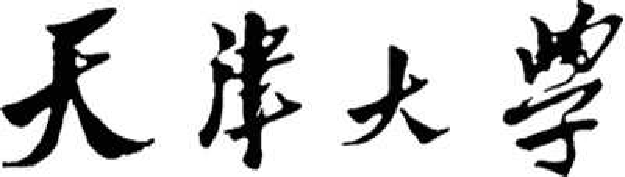
\includegraphics[width=0.4\textwidth]{figures/tju}
      \end{figure}
      \vspace*{15pt}
      \hei\erhao{\textbf{\@ccovertitle}} \\
      \hei\erhao{\textbf{\@ctitle}}
      \vspace*{55pt}

      \begin{figure}[H]
      \centering
      
\includegraphics[width=0.3\textwidth]{figures/Tjulogo}
      \end{figure}

      \vspace*{60pt}
      \song\sanhao{小组成员：杨博~~~牛文航~~~魏语菲~~~任晓华~~~陈宇泽}
      \vspace*{40pt}

    \song\sanhao{\textbf{\@cdate}}
    \end{center}
    \end{titlepage}
}
                             % 完成对论文各个部分格式的设置
	% !Mode:: "TeX:UTF-8"


%%%%%%%%%%%%%%%%%%%%%%%%%%%%%%%%%%%%%%%%%%%%%%%%%%%%%%%%%%%%%%%
%%  可通过对 setup/format.tex中                               %%
%%  第243行 \setlength{\@title@width}{5cm}中 5cm 这个参数来   %%
%%  控制封面中下划线的长度。                                   %%
%%%%%%%%%%%%%%%%%%%%%%%%%%%%%%%%%%%%%%%%%%%%%%%%%%%%%%%%%%%%%%

\cheading{天津大学软件学院《软件工程高级实践》结课报告}      % 正文页眉
\ccovertitle{《软件工程高级实践》结课报告}                       % 封面标题

%%%%%%%%%%%%%%%%%%%%%%%%%%%%%%%%%%%%%%%%%%%%%%%%%%%%%%%%%%%%%
%%%%%%%%%% 以下为论文的基本信息，需要由作者进行修改 %%%%%%%%%%%%
%%%%%%%%%%%%%%%%%%%%%%%%%%%%%%%%%%%%%%%%%%%%%%%%%%%%%%%%%%%%%

\caffil{软件学院}       % 学院名称
\csubject{软件工程}     % 专业名称
\cgrade{2023级}           % 年级

\cdate{\the\year~年~\the\month~月~\the\day~日}  % 论文完成日期，不需要修改，自动生成

	\frontmatter                                     % 以下是论文导言部分，包括论文的封面，中英文摘要和中文目录
	\fancypagestyle{plain}{							 % 正文前均无页眉
		\fancyhf{}
		\renewcommand{\headrulewidth}{0 pt}
		\fancyfoot[C]{\song\xiaowu~\thepage~}
	}

	\makecover 			% 封面

	\include{setup/toc} % 目录

	\mainmatter\defaultfont\sloppy\raggedbottom
	\makeatletter
	\fancypagestyle{plain}{                              % 设置正文眉页脚风格
		\fancyhf{}
		\fancyhead[C]{\song\wuhao \@cheading}            % 页眉格式
		\fancyfoot[C]{\song\xiaowu ~\thepage~}           % 页脚格式
		\renewcommand{\headrulewidth}{0.5pt}
		\renewcommand{\footrulewidth}{0pt}
	}
	\makeatother
	\setcounter{page}{1}                                 % 单独从 1 开始编页码
	\titleformat{\chapter}{\centering\xiaosan\hei}{\chaptername}{2em}{} % 恢复chapter标题格式要求

	%%%%%% 这里是正文，每个文件对应正文中的一章 %%%%%%
	% !Mode:: "TeX:UTF-8"

\chapter{需求分析}

\section{项目背景}

本项目是"饿了么"外卖点餐平台的微服务化实现，基于Spring Cloud + Vue前后端分离架构。系统围绕外卖点餐的核心业务流程，涵盖用户注册登录、商家浏览、食品选择、购物车管理、订单创建与支付、虚拟钱包、积分系统等功能模块。

本项目开发了一个完整的外卖点餐平台"点餐业务线"整体流程。项目要求采用微服务架构，使用Spring Cloud技术栈实现服务治理、通信、容错等核心机制。

\section{功能性需求分析}

根据项目任务书及业务分析，系统需支持以下功能模块。

\subsection{用户服务模块}

\begin{itemize}
	\item 用户注册：支持用户名、密码、性别等基本信息的注册，密码使用BCrypt加密存储
	\item 用户登录：基于JWT（JSON Web Token）的身份认证机制，支持"记住我"延长令牌有效期
	\item 用户信息管理：查看个人信息、修改密码、更新用户资料
	\item 生日设置：用于生日积分奖励的判断依据
	\item 用户查询：支持按ID查询、按用户名查询、检查用户是否存在
\end{itemize}

\subsection{商家服务模块}

\begin{itemize}
	\item 商家列表查询：按分类展示所有商家信息
	\item 商家详情查询：获取特定商家的完整信息，包括名称、地址、起送价、配送费等
	\item 商家注册与管理：支持商家入驻注册和管理自己的店铺
	\item 订单类型管理：按商家分类管理订单类型
\end{itemize}

\subsection{食品服务模块}

\begin{itemize}
	\item 食品CRUD操作：食品的创建、查询、更新、删除（逻辑删除，设置valid=0）
	\item 按商家查询食品：获取特定商家下的所有在售食品
	\item 商家关联验证：通过Feign调用商家微服务，验证食品所属商家是否存在
\end{itemize}

\subsection{购物车服务模块}

\begin{itemize}
	\item 购物车添加：将食品加入购物车，若已存在则更新数量
	\item 购物车管理：查询、更新数量、删除购物车项
	\item 多维度查询：支持按用户ID和按商家ID两个维度查询购物车内容
	\item 订单创建联动：下单成功后自动清空对应的购物车项
\end{itemize}

\subsection{订单服务模块}

\begin{itemize}
	\item 订单创建：从购物车批量创建订单，包含订单明细（订单主体\&订单详单）
	\item 订单查询：支持按用户ID、按商家ID、按订单ID多维度查询
	\item 订单状态流转：待支付(0)→已支付(1)→配送中(2)→已完成(3)
	\item 虚拟钱包支付：通过虚拟钱包余额+积分抵扣组合支付
	\item 分布式锁保障：支付环节使用Redisson分布式锁，确保金钱交易一致性
\end{itemize}

\subsection{配送地址服务模块}

\begin{itemize}
	\item 配送地址CRUD：新增、修改、删除配送地址
	\item 按用户查询：获取某用户的所有有效配送地址
	\item 逻辑删除：删除操作不物理删除数据，仅设置valid=0
\end{itemize}

\subsection{虚拟钱包服务模块}

\begin{itemize}
	\item 钱包自动创建：用户注册后自动创建虚拟钱包
	\item 核心操作：余额查询、充值、支付、转账
	\item 透支管理：支持信用额度透支与还款
	\item 交易明细记录：记录所有交易的金额、类型、时间、对方钱包
\end{itemize}

\subsection{VIP卡服务模块}

\begin{itemize}
	\item VIP卡购买：提供99元和299元两档VIP卡
	\item 信用额度：VIP用户获得2000元信用额度
	\item VIP卡状态管理：记录购买时间、到期时间、状态
\end{itemize}

\subsection{积分服务模块}

\begin{itemize}
	\item 积分多渠道获取：签到奖励、消费返积分、活动赠送、生日奖励、红包雨
	\item 积分消费：订单抵扣、积分兑换
	\item 积分统计：按可用/已用/已过期维度进行统计分析
	\item 定时任务：每日凌晨自动处理积分过期，每日凌晨发放生日积分
	\item 红包雨活动：支持红包雨促销活动的配置与管理
\end{itemize}

\section{非功能性需求}

\subsection{性能需求}

\begin{itemize}
	\item 网关层引入响应缓存机制：对商家和食品等低频变更数据的GET请求进行缓存，减少重复的微服务调用，将响应时间从秒级缩短至毫秒级
	\item 数据库连接池复用：减少连接创建与销毁的开销
	\item 使用消息队列实现异步通信：提升系统吞吐量，降低同步调用链路的延迟
\end{itemize}

\subsection{安全需求}

\begin{itemize}
	\item JWT令牌认证：所有API请求需携带有效Token，令牌使用HMAC-SHA512算法签名
	\item BCrypt密码加密存储：用户密码不以明文形式存储
	\item 网关统一入口：隐藏内部微服务拓扑，对外部仅暴露网关端口
	\item 前后端分离：前端通过网关代理访问后端，避免直接暴露微服务地址
\end{itemize}

\subsection{可用性需求}

\begin{itemize}
	\item 服务注册与发现机制：支持服务实例动态上下线，无需手动配置
	\item 网关层熔断降级：保证每个请求都能获得响应，即使后端服务故障也不返回白屏
	\item Feign客户端集成降级回退逻辑：微服务间调用失败时有兜底处理
	\item 高可用集群设计：Eureka Server集群部署，避免单点故障
\end{itemize}

\subsection{可维护性}

\begin{itemize}
	\item 集中配置管理：所有微服务的配置文件统一托管在Config Server
	\item 基于Spring Cloud Bus的配置动态刷新：修改配置无需重启服务
	\item RESTful API规范化设计：前后端通过《接口规格说明书》解耦并行开发
	\item 代码模块化：每个微服务独立管理，职责清晰
\end{itemize}

\subsection{可扩展性}

\begin{itemize}
	\item 微服务独立部署与独立扩展：可根据业务压力针对性地对特定服务进行横向扩展
	\item 服务间通过Feign声明式调用：无硬编码URL，服务位置透明
	\item 数据库按业务域垂直拆分：每个微服务使用独立的数据库，避免数据耦合
\end{itemize}

\subsection{数据一致性}

\begin{itemize}
	\item 涉及金钱的业务（钱包充值/支付/转账、订单支付、积分扣减）使用Redisson分布式锁保障严格一致性
	\item 订单支付流程使用Spring事务保护，确保订单创建与购物车清空的原子性
	\item 非金融类业务（如订单状态通知）采用RabbitMQ消息队列实现最终一致性
\end{itemize}
    % 需求分析
	% !Mode:: "TeX:UTF-8"

\chapter{项目架构设计}

\section{总体架构}

系统采用五层架构设计，自顶向下分为：前端层、网关层、业务层、数据访问层和基础设施层。

\subsection{前端层}

前端层使用Vue.js 3框架构建单页面应用（SPA），结合Element Plus组件库提供用户界面。前端通过Axios HTTP客户端向网关统一入口发起请求，使用Vue Router管理路由，ECharts实现数据可视化。前端开发服务器运行在端口8081，生产环境通过Nginx部署。

\subsection{网关层}

网关层基于Spring Cloud Gateway构建，作为系统的唯一入口，负责以下核心职责：
\begin{itemize}
	\item 请求路由：根据请求路径将请求转发到对应的微服务
	\item 负载均衡：通过Spring Cloud LoadBalancer实现客户端负载均衡
	\item 熔断降级：基于Resilience4j为每个后端服务配置独立的熔断器
	\item 自定义缓存：为商家和食品的GET请求实现网关级响应缓存
	\item 全局CORS：配置跨域资源共享策略
\end{itemize}

\subsection{业务层}

业务层包含8个独立微服务，按业务域垂直拆分。每个微服务独立部署、独立扩展，拥有独立的数据库。微服务之间通过以下两种方式通信：
\begin{itemize}
	\item 同步调用：通过OpenFeign声明式HTTP客户端进行同步的服务间调用
	\item 异步消息：通过RabbitMQ消息队列进行异步的订单状态变更通知
\end{itemize}

\subsection{数据访问层}

数据访问层包含MySQL和Redis两种数据存储：
\begin{itemize}
	\item MySQL 8.0：存储各业务域的持久化数据，每个微服务使用独立数据库
	\item Redis 6.2：通过Redisson客户端实现分布式锁，保障金钱交易的一致性
\end{itemize}

\subsection{基础设施层}

基础设施层为整个微服务架构提供支撑能力：
\begin{itemize}
	\item Eureka Server：服务注册与发现中心
	\item Spring Cloud Config Server：集中配置管理
	\item RabbitMQ：消息中间件，支持Spring Cloud Bus配置刷新和异步消息通信
	\item Docker Compose：容器化部署MySQL、Redis、RabbitMQ
\end{itemize}

\section{技术选型}

系统技术栈的选择遵循以下原则：使用业界成熟的微服务框架、优先采用Spring Cloud生态组件、保证技术栈的一致性和可维护性。

\begin{table}[H]
	\centering
	\caption{技术选型一览表}
	\begin{tabular}{p{4.0cm}p{5.0cm}p{5.0cm}}
		\hline
		\textbf{层面} & \textbf{技术} & \textbf{版本} \\
		\hline
		开发框架 & Spring Boot & 2.4.5 \\
		微服务框架 & Spring Cloud & 2020.0.2 \\
		服务注册与发现 & Netflix Eureka & -- \\
		配置中心 & Spring Cloud Config & -- \\
		API网关 & Spring Cloud Gateway & -- \\
		服务间调用 & OpenFeign & -- \\
		客户端负载均衡 & Spring Cloud LoadBalancer & -- \\
		熔断降级 & Resilience4j & -- \\
		配置刷新总线 & Spring Cloud Bus & -- \\
		消息队列 & RabbitMQ & 3.13 \\
		数据库 & MySQL & 8.0.36 \\
		缓存/分布式锁 & Redis + Redisson & 6.2.14 / 3.16.8 \\
		认证授权 & JWT (jjwt) & 0.11.5 \\
		前端框架 & Vue 3 + Element Plus & -- \\
		\hline
	\end{tabular}
\end{table}

\section{模块划分与服务端口}

系统共包含11个独立部署的模块，每个模块有明确的职责和固定的端口分配。

\begin{table}[H]
	\centering
	\caption{模块划分与服务端口}
	\begin{tabular}{p{5.5cm}p{2.5cm}p{6.0cm}}
		\hline
		\textbf{模块名称} & \textbf{端口} & \textbf{职责} \\
		\hline
		elm-eureka-server & 13000 & 服务注册中心 \\
		elm-config-server & 15001 & 集中配置管理 \\
		elm-gateway-server & 14000 & API网关 \\
		elm-user-server & 10100 & 用户管理与JWT认证 \\
		elm-business-server & 10400 & 商家管理与订单生命周期 \\
		elm-food-server & 10200 & 食品管理 \\
		elm-cart-server & 10300 & 购物车管理 \\
		elm-order-server & 11000 & 订单创建与支付 \\
		elm-delivery-server & 10500 & 配送地址管理 \\
		elm-wallet-server & 18000 & 虚拟钱包与VIP \\
		elm-point-server & 15008 & 积分与促销活动 \\
		\hline
	\end{tabular}
\end{table}

\section{微服务依赖关系}

系统严格遵循无循环依赖原则，服务间的依赖方向为单向。订单服务是系统中依赖最多的节点，它通过Feign客户端分别调用购物车服务、钱包服务、积分服务和商家服务。食品服务通过Feign调用商家服务以验证商家是否存在。钱包服务通过Feign调用用户服务以验证用户身份。所有Feign调用方向均为单向，严格避免了循环依赖。

异步通信方面：商家服务在订单状态变更时通过RabbitMQ发出消息，购物车服务订阅该消息，实现解耦的异步通知。

\section{RESTful API设计规范}

本项目对所有业务接口进行了RESTful规范化重构，核心思想是将数据库表项视为"资源"，URL表示资源路径，HTTP方法表示对资源的操作。

与教学视频中混用动词短语和路径参数的接口设计不同，我们严格遵循以下规范：

\begin{itemize}
	\item 使用复数名词表示资源集合：\verb|/businesses|、\verb|/foods|、\verb|/orders|
	\item 使用HTTP方法表达操作语义：GET（获取）、POST（创建）、PUT（更新）、DELETE（删除）
	\item 通过路径参数标识具体资源：\verb|/businesses/{businessId}|
	\item 通过查询参数传递筛选条件：\verb|/foods?businessId={id}|
	\item 统一响应格式：\verb|CommonResult(code, message, result)|
\end{itemize}

团队为此编写了《RESTful API接口规格说明书》，详细规定了每个接口的请求方法、资源路径格式、请求参数、响应格式和错误码语义。这为前后端并行开发提供了契约基础——前端开发人员只需依据接口文档即可进行开发，无需等待后端接口完成。

\section{业务对象设计优化}

\subsection{金额类型优化}

教学视频中商品价格、配送费等金额属性使用了\verb|double|类型。然而\verb|float|和\verb|double|类型的尾数位数固定，对于需要精确表示的小数（如0.10元），\verb|double|类型无法精确表示，这在金融数据处理中是绝对不允许的。本项目将所有金额相关的属性统一替换为\verb|BigDecimal|类型，确保金额运算的精度。

\subsection{对象关联方式优化}

教学视频中业务对象之间存在直接嵌套关系：Order对象中包含Business对象和Cart列表，Cart中包含Food对象，Food中又包含Business对象。这种深度嵌套导致一个订单的响应体动辄数MB（因为包含多张Base64编码的图片），在远程部署环境下单个请求耗时可达5-8秒。

本项目将对象之间的关联改为通过主键引用：Order存储businessId和foodId列表，Cart存储foodId，Food存储businessId。这一重构将订单响应大小从MB级降至KB级，显著提升了响应速度，同时降低了微服务之间的耦合度。
    % 项目架构设计
	% !Mode:: "TeX:UTF-8"

\chapter{基于Eureka的服务注册与发现及高可用集群}

\section{Eureka服务注册与发现}

\subsection{设计原理}

Eureka是Netflix开源的服务注册与发现组件，采用AP架构（可用性 + 分区容错性），是Spring Cloud微服务治理的核心组件。Eureka包含两个核心角色：

\begin{itemize}
	\item \textbf{Eureka Server（服务注册中心）}：维护所有已注册服务实例的注册表，接收客户端的注册请求和心跳续约，通过REST API对外暴露服务列表
	\item \textbf{Eureka Client（服务客户端）}：启动时向Server注册自身信息，定期发送心跳以维持租约，定期从Server拉取服务注册表到本地缓存
\end{itemize}

\subsection{Eureka Server实现}

本项目的Eureka Server位于elm-eureka-server模块，启动类通过\verb|@EnableEurekaServer|注解启用服务注册中心功能。其核心配置如下：

\begin{lstlisting}[language=Java, caption=Eureka Server配置]
server:
  port: 13000
eureka:
  instance:
    hostname: 127.0.0.1
  client:
    register-with-eureka: false   # 不向自身注册
    fetch-registry: false         # 不从自身拉取注册表
    service-url:
      defaultZone: http://${eurekahost2}:${server.port}/eureka/
\end{lstlisting}

关键配置说明：
\begin{itemize}
	\item \verb|register-with-eureka: false|：Eureka Server自身不需要被注册到注册中心
	\item \verb|fetch-registry: false|：Eureka Server不需要从自身拉取服务列表
	\item \verb|defaultZone| 配置了同伴节点的地址，为Eureka集群做准备
\end{itemize}

\subsection{Eureka Client实现}

所有业务微服务通过引入\verb|spring-cloud-starter-netflix-eureka-client|依赖并使用\verb|@EnableEurekaClient|注解，即可在启动时自动注册到Eureka Server。各微服务的bootstrap.yml中配置了Eureka Client参数：

\begin{lstlisting}[language=Java, caption=Eureka Client配置]
eureka:
  client:
    service-url:
      defaultZone: http://127.0.0.1:13000/eureka/
  instance:
    prefer-ip-address: true
    lease-renewal-interval-in-seconds: 5      # 心跳间隔5秒
    lease-expiration-duration-in-seconds: 15  # 租约过期时间15秒
\end{lstlisting}

心跳机制保证服务实例的活性：客户端每5秒向Server发送一次心跳续约，若Server在15秒内未收到心跳，则将该实例从注册表中剔除。

\section{Eureka高可用集群设计}

\subsection{设计动机}

单点Eureka Server存在单点故障风险：一旦该Server宕机，新服务无法注册，现有服务无法发现其他服务实例。虽然已拉取了注册表的客户端可以继续使用本地缓存进行服务调用，但系统的弹性将受到严重影响。

\subsection{集群架构}

Eureka通过Peer-to-Peer机制实现高可用。部署多个Eureka Server实例，它们互相注册形成对等关系。本项目配置了两个Eureka节点，通过\verb|defaultZone|互相指向对方实现集群：

\begin{lstlisting}[language=Java, caption=Eureka集群Client配置]
eureka:
  client:
    service-url:
      defaultZone: http://host1:13000/eureka/,http://host2:13000/eureka/
\end{lstlisting}

各微服务同时向两个注册中心注册，即使一个Eureka Server宕机，微服务仍可从另一个Server获取服务注册表，保证了服务发现的高可用性。

\subsection{自我保护机制}

Eureka Server默认开启自我保护模式。当Server在短时间内丢失大量心跳续约时，会进入自我保护状态，不再剔除任何服务实例。这一设计避免因网络瞬时故障导致大量服务被错误剔除。本项目保留了此机制，以保证系统的健壮性。
    % Eureka服务注册与发现及高可用集群
	% !Mode:: "TeX:UTF-8"

\chapter{基于HTTP的客户端负载均衡}

\section{设计原理}

在微服务架构中，同一服务通常部署多个实例以提高可用性和吞吐量。负载均衡机制负责将请求合理分配到各个服务实例上。客户端负载均衡将负载均衡逻辑集成在服务调用方，调用方从服务注册中心获取目标服务的所有实例列表，然后根据均衡策略自主选择一个实例发起调用。

在Spring Cloud生态中，Netflix Ribbon是经典的客户端负载均衡组件。但在Spring Cloud 2020.0.2版本中，Ribbon已进入维护模式，官方推荐使用Spring Cloud LoadBalancer作为替代方案。两者的核心设计思想一致：在客户端实现负载均衡策略，避免引入额外的网络跳转。

\section{Spring Cloud LoadBalancer实现}

\subsection{Gateway中的负载均衡}

Gateway的所有路由规则中，目标URI均使用\verb|lb://|前缀：

\begin{lstlisting}[language=Java, caption=Gateway路由中的负载均衡]
routes:
  - id: userServer
    uri: lb://elm-user-server    # lb:// 前缀启用负载均衡
    predicates:
      - Path=/users/**
\end{lstlisting}

当Gateway收到匹配的请求时，会通过负载均衡器从Eureka注册表中获取对应服务的所有健康实例列表，然后根据轮询策略选择一个实例转发请求。

\subsection{Feign中的负载均衡}

所有Feign客户端定义的\verb|@FeignClient(name = "elm-business-server")|中的\verb|name|属性即对应Eureka中的服务名。Feign内部集成了Spring Cloud LoadBalancer，在发起HTTP调用时自动实现负载均衡：

\begin{lstlisting}[language=Java, caption=Feign集成LoadBalancer]
@FeignClient(name = "elm-business-server")
public interface BusinessClient {
    @GetMapping("/businesses/{businessId}")
    String getBusinessById(@PathVariable("businessId") Integer businessId);
}
\end{lstlisting}

当调用\verb|BusinessClient.getBusinessById(1)|时，Feign自动从Eureka本地缓存中查找\verb|elm-business-server|的所有实例，通过LoadBalancer选择一个健康实例并发起HTTP请求，整个过程对开发者完全透明。

\subsection{Eager Load配置}

为避免首次请求的冷启动延迟，Gateway配置了急切加载：

\begin{lstlisting}[language=Java, caption=Eager Load配置]
spring:
  cloud:
    gateway:
      loadbalancer:
        eager-load:
          clients:
            - elm-user-server
            - elm-business-server
            - elm-food-server
            - elm-cart-server
            - elm-delivery-server
            - elm-order-server
            - elm-point-server
            - elm-wallet-server
\end{lstlisting}

Eager Load使Gateway在启动时即预加载所有目标服务的实例列表，消除首次请求的延迟。

\section{Ribbon到Spring Cloud LoadBalancer的演进}

Spring Cloud 2020.0.2中Ribbon已被Spring Cloud LoadBalancer取代，原因包括：Ribbon自2018年起进入维护模式；Spring Cloud LoadBalancer是Spring官方维护方案，与Spring Cloud Gateway的非阻塞架构天然匹配；虽然底层组件变化，但客户端负载均衡的核心思想保持不变。
    % 客户端负载均衡（Ribbon/LoadBalancer）
	% !Mode:: "TeX:UTF-8"

\chapter{基于Feign的声明式服务调用}

\section{设计原理}

Feign是Netflix开发的声明式HTTP客户端，通过"接口 + 注解"的编程模型大幅简化了服务间调用代码。其核心优势包括：

\begin{itemize}
	\item \textbf{声明式编程模型}：只需定义Java接口并标注注解，Feign自动生成代理实现类
	\item \textbf{内置负载均衡}：集成Spring Cloud LoadBalancer，自动实现客户端负载均衡
	\item \textbf{集成熔断降级}：通过\verb|fallback|属性指定降级实现类
	\item \textbf{契约驱动}：Feign接口定义本身就是服务调用契约
\end{itemize}

\section{Feign客户端定义}

项目中共定义了9个Feign客户端，涵盖所有跨服务调用场景：

\begin{table}[H]
	\centering
	\caption{Feign客户端总览}
	\begin{tabular}{p{3.5cm}p{3.0cm}p{4.0cm}}
		\hline
		\textbf{客户端} & \textbf{所在服务} & \textbf{目标服务与用途} \\
		\hline
		BusinessClient & food-server & business-server：验证商家存在 \\
		FoodFeignClient & cart-server & food-server：获取食品信息 \\
		OrderFeignClient & cart-server & business-server：创建订单 \\
		BusinessClient & order-server & business-server：获取商家信息 \\
		CartClient & order-server & cart-server：购物车操作 \\
		PointClient & order-server & point-server：积分操作 \\
		VirtualWalletClient & order-server & wallet-server：余额、转账 \\
		UserClient & wallet-server & user-server：验证用户存在 \\
		OrderClient & point-server & order-server：关联订单积分 \\
		\hline
	\end{tabular}
\end{table}

以下以订单服务调用钱包服务为例：

\begin{lstlisting}[language=Java, caption=VirtualWalletClient.java]
@FeignClient(name = "elm-wallet-server")
public interface VirtualWalletClient {
    @GetMapping("/wallet/getBalance")
    CommonResult<BigDecimal> getBalanceByUserId(
        @RequestParam("userId") String userId);

    @PostMapping("/wallet/transfer")
    CommonResult<Integer> transfer(
        @RequestParam("fromUserId") String fromUserId,
        @RequestParam("toUserId") String toUserId,
        @RequestParam("amount") BigDecimal amount);
}
\end{lstlisting}

\section{Feign集成Fallback降级}

当目标服务不可用时，Feign通过\verb|fallback|属性调用降级实现类，返回兜底数据：

\begin{lstlisting}[language=Java, caption=Feign Fallback降级]
@FeignClient(name = "elm-business-server",
             fallback = BusinessClientFallback.class)
public interface BusinessClient {
    @GetMapping("/businesses/{businessId}")
    String getBusinessById(@PathVariable("businessId") Integer businessId);
}

@Component
public class BusinessClientFallback implements BusinessClient {
    @Override
    public String getBusinessById(Integer businessId) {
        return "{\"code\":200, " +
               "\"message\":\"Fallback: Business service unavailable\"}";
    }
}
\end{lstlisting}

食品服务调用商家服务验证商家是否存在时，若商家服务不可用，Fallback返回模拟的成功响应，使食品服务仍能正常运行（宽松策略，假设商家存在）。这种设计体现了微服务架构中"优雅降级"的思想。

\section{组合调用示例}

订单服务创建订单时，组合使用多个Feign客户端：

\begin{lstlisting}[language=Java, caption=订单创建中的Feign组合调用]
@Transactional
public int createOrders(Orders orders) {
    // 1. Feign获取购物车
    CommonResult<?> cartResult =
        cartClient.listCart(orders.getUserId(), orders.getBusinessId());
    // 2. 创建订单主记录与明细
    ordersMapper.saveOrders(orders);
    orderDetailetMapper.saveOrderDetailetBatch(list);
    // 3. Feign清空购物车
    cartClient.removeCart(orders.getUserId(), orders.getBusinessId());
    return orderId;
}
\end{lstlisting}

整个过程是声明式的——开发者只需关注业务逻辑，HTTP通信的细节完全由Feign处理。
    % Feign声明式服务调用
	% !Mode:: "TeX:UTF-8"

\chapter{延迟与容错：从Hystrix到Resilience4j}

\section{设计原理}

在微服务架构中，当某个服务出现故障或响应缓慢时，如果不加以控制，故障会通过调用链向上游传播，最终导致整个系统的"雪崩效应"。熔断器（Circuit Breaker）模式是预防雪崩效应的核心手段。

熔断器有三种状态：
\begin{description}
	\item[CLOSED（闭合状态）] 所有请求正常通过。当失败率超过阈值时切换到OPEN
	\item[OPEN（断开状态）] 请求直接失败（短路），执行降级逻辑。经过等待时间后切换到HALF\_OPEN
	\item[HALF\_OPEN（半开状态）] 允许部分请求试探通过。成功则回到CLOSED，失败则回到OPEN
\end{description}

Hystrix是Netflix开源的传统熔断器组件，但在Spring Cloud 2020.0.2中已被移除。本项目使用Resilience4j作为替代方案，应用于Gateway网关层。

\section{Gateway层熔断器配置}

\begin{lstlisting}[language=Java, caption=CircuitBreakerConfig.java]
@Configuration
public class CircuitBreakerConfig {
    @Bean
    public ReactiveResilience4JCircuitBreakerFactory
            reactiveResilience4JCircuitBreakerFactory() {
        ReactiveResilience4JCircuitBreakerFactory factory =
            new ReactiveResilience4JCircuitBreakerFactory();
        TimeLimiterConfig timeLimiterConfig = TimeLimiterConfig.custom()
                .timeoutDuration(Duration.ofSeconds(20))
                .cancelRunningFuture(true)
                .build();
        factory.configure(
            builder -> builder.timeLimiterConfig(timeLimiterConfig).build(),
            "globalCircuitBreaker", "userCircuitBreaker",
            "businessCircuitBreaker", "foodCircuitBreaker",
            "cartCircuitBreaker", "orderCircuitBreaker",
            "deliveryCircuitBreaker", "walletCircuitBreaker",
            "pointCircuitBreaker"
        );
        return factory;
    }
}
\end{lstlisting}

设计要点：
\begin{itemize}
	\item \textbf{独立熔断器}：为9个服务分别创建独立的熔断器，确保某个服务熔断不影响其他服务
	\item \textbf{统一超时}：所有熔断器配置20秒超时，超时后触发熔断
	\item \textbf{取消运行中的Future}：\verb|cancelRunningFuture(true)|确保超时后释放线程资源
\end{itemize}

\section{路由中的熔断器集成}

Gateway的每条路由规则都配置了CircuitBreaker过滤器和对应的降级处理地址：

\begin{lstlisting}[language=Java, caption=路由中的熔断器配置]
routes:
  - id: userServer
    uri: lb://elm-user-server
    filters:
      - name: CircuitBreaker
        args:
          name: userCircuitBreaker
          fallbackUri: forward:/userFallback
\end{lstlisting}

\section{降级响应设计}

FallbackController为每个微服务定义降级处理方法：

\begin{lstlisting}[language=Java, caption=FallbackController降级响应]
@RequestMapping("/userFallback")
@ResponseStatus(HttpStatus.FORBIDDEN)
public CommonResult<Map<String, Object>> userFallback(
        ServerWebExchange exchange) {
    Map<String, Object> metadata = new LinkedHashMap<>();
    metadata.put("fallback", true);      // 标记为熔断响应
    metadata.put("service", "user");     // 标识故障服务
    metadata.put("retryable", true);     // 标记可重试
    metadata.put("path", exchange.getRequest().getURI().getRawPath());
    return new CommonResult<>(403,
        "Gateway触发了用户微服务的熔断降级方法.", metadata);
}
\end{lstlisting}

降级响应携带丰富元数据：\verb|fallback: true|让前端判断这是熔断响应而非业务错误；\verb|retryable: true|提示可重试；\verb|path|和\verb|method|记录原始请求信息便于排查。

\section{容错机制分层总结}

系统的容错机制分为两层：
\begin{enumerate}
	\item \textbf{Gateway层熔断（Resilience4j）}：超时20秒触发，返回FallbackController降级响应，HTTP状态码403
	\item \textbf{Feign层降级（Fallback实现类）}：当目标微服务不可达时，调用Fallback方法返回兜底数据
\end{enumerate}

两层容错互为补充：Gateway层保障外部请求的可用性，Feign层保障内部服务间调用的鲁棒性。
    % 延迟与容错（Hystrix/Resilience4j）
	% !Mode:: "TeX:UTF-8"

\chapter{基于Spring Cloud Gateway的微服务网关}

\section{设计原理}

Spring Cloud Gateway是Spring官方基于Spring WebFlux构建的API网关，采用非阻塞I/O（Netty），能以少量线程处理大量并发连接。其核心组件包括：

\begin{itemize}
	\item \textbf{Route（路由）}：网关的基本构建块，包含ID、目标URI、Predicate集合和Filter集合
	\item \textbf{Predicate（断言）}：基于Java 8的Predicate，匹配HTTP请求的路径、Header、参数等属性
	\item \textbf{Filter（过滤器）}：对请求/响应进行处理，分为GatewayFilter和GlobalFilter
\end{itemize}

\section{Gateway路由设计}

项目共配置了15条路由规则，每个业务微服务对应两条路由——一条匹配直接路径，另一条匹配\verb|/api/|前缀路径：

\begin{table}[H]
	\centering
	\caption{Gateway路由规则一览}
	\begin{tabular}{p{4.0cm}p{4.5cm}p{4.0cm}}
		\hline
		\textbf{路由ID} & \textbf{路径匹配} & \textbf{目标服务} \\
		\hline
		userServer / userApiServer & /users/**, /api/auth... & user-server \\
		businessServer / businessApiServer & /businesses/**, /api/businesses/** & business-server \\
		cartServer / cartApiServer & /carts/**, /api/carts/** & cart-server \\
		deliveryServer / deliveryApiServer & /delivery-addresses/** & delivery-server \\
		ordersServer / ordersApiServer & /orders/**, /api/orders/** & order-server \\
		pointServer / pointApiServer & /points/**, /api/points/** & point-server \\
		foodServer / foodApiServer & /foods/**, /api/foods/** & food-server \\
		walletServer / walletApiServer & /wallet/**, /api/wallet/** & wallet-server \\
		\hline
	\end{tabular}
\end{table}

\verb|/api/|前缀路由使用RewritePath过滤器去除前缀：前端请求\verb|GET /api/businesses/1|，网关将其重写为\verb|/businesses/1|后转发到后端。

\begin{lstlisting}[language=Java, caption=路径重写过滤器]
filters:
  - RewritePath=/api/(?<segment>.*), /${segment}
\end{lstlisting}

\section{全局配置}

\begin{lstlisting}[language=Java, caption=CORS与超时配置]
spring:
  cloud:
    gateway:
      httpclient:
        connect-timeout: 20000    # 连接超时20秒
        response-timeout: 20s     # 响应超时20秒
      globalcors:
        cors-configurations:
          '[/**]':
            allowedOrigins: "*"
            allowedHeaders: "*"
            allowedMethods: "*"
\end{lstlisting}

\section{自定义缓存过滤器（项目特色）}

\subsection{设计动机}

商家列表包含图片信息，每个约200KB，在远程部署环境下每次获取需要约4秒。然而商家信息变化概率很小，但读取请求非常频繁。基于"读多写少"的特点，我们在网关层为商家和食品的GET请求实现了缓存机制。

\subsection{实现方案}

缓存机制通过自定义GatewayFilter实现：

\begin{lstlisting}[language=Java, caption=BusinessCacheGet过滤器]
@Component
public class BusinessCacheGetGatewayFilterFactory
        extends AbstractGatewayFilterFactory<Object> {
    private static final String PATH_PATTERN = "businesses/(\\d+)";

    @Override
    public GatewayFilter apply(Object config) {
        return (exchange, chain) -> {
            String path = exchange.getRequest().getURI().getPath();
            Matcher matcher = Pattern.compile(PATH_PATTERN).matcher(path);
            if (matcher.find()) {
                Integer businessId = Integer.valueOf(matcher.group(1));
                if (BusinessCache.businessMap.containsKey(businessId)) {
                    // 缓存命中，直接从网关返回
                    return exchange.getResponse().writeWith(
                        Mono.just(exchange.getResponse().bufferFactory()
                            .wrap(BusinessCache.businessMap
                                .get(businessId).getBytes()))
                    );
                }
            }
            return chain.filter(exchange); // 未命中，继续转发
        };
    }
}
\end{lstlisting}

\subsection{缓存策略}

\begin{table}[H]
	\centering
	\caption{网关缓存策略}
	\begin{tabular}{p{5.0cm}p{10.0cm}}
		\hline
		\textbf{请求类型} & \textbf{缓存行为} \\
		\hline
		GET 单个商家/食品 & 未命中→转发后端→Post过滤器缓存响应；命中→直接从网关返回 \\
		PUT/POST/DELETE & 修改操作触发时清除本地对应缓存条目 \\
		\hline
	\end{tabular}
\end{table}

此设计将重复GET请求的响应时间从秒级（需经过完整网络链路）降至毫秒级（网关内存操作）。
    % Spring Cloud Gateway微服务网关
	% !Mode:: "TeX:UTF-8"

\chapter{集中配置管理与配置刷新}

\section{基于Spring Cloud Config的集中配置管理}

\subsection{设计原理}

在微服务架构中，每个服务都有自己的配置文件。当服务数量增多时，分散的配置文件难以管理和维护。Spring Cloud Config提供Server-Client模式的集中配置管理方案：

\begin{itemize}
	\item \textbf{Config Server}：从Git仓库或本地文件系统读取配置文件，通过REST API对外暴露
	\item \textbf{Config Client}：启动时从Config Server拉取配置，再初始化自己的Spring上下文
\end{itemize}

\subsection{Config Server实现}

本项目Config Server使用native模式（本地文件系统），配置文件存储在\verb|elm-configs/|目录下：

\begin{lstlisting}[language=Java, caption=Config Server配置]
server:
  port: 15001
spring:
  profiles:
    active: native
  cloud:
    config:
      server:
        native:
          search-locations: file:///E:/ELM-CLOUD/elm-configs
\end{lstlisting}

配置文件以\verb|{application-name}-{profile}.yml|格式命名，包括所有8个业务微服务和网关的配置。

\subsection{Config Client配置}

各微服务通过bootstrap.yml从Config Server拉取配置：

\begin{lstlisting}[language=Java, caption=Config Client bootstrap.yml]
spring:
  cloud:
    config:
      name: elm-user-server-1    # 配置文件名称
      profile: dev                # 环境
      label: elm-configs          # 标签
      uri: http://localhost:15001 # Config Server地址
\end{lstlisting}

\subsection{参数化配置}

配置文件中使用环境变量占位符，支持不同环境灵活配置：

\begin{lstlisting}[language=Java, caption=参数化配置示例]
spring:
  datasource:
    username: ${DB_USER:root}
    password: ${DB_PASSWORD:123456}
    url: jdbc:mysql://${DB_HOST:localhost}:${DB_PORT:3306}/${DB_NAME:elm2}
\end{lstlisting}

\subsection{Gateway路由外部化}

Gateway的全部15条路由规则均存储在Config Server中，而非Gateway本地配置文件。这样可以在不重启Gateway的情况下，通过配置刷新机制更新路由规则。

\section{基于Spring Cloud Bus的配置刷新}

\subsection{设计原理}

当Config Server中的配置发生变化时，需要通知各微服务刷新配置。Spring Cloud Bus利用RabbitMQ等消息中间件作为通信总线，实现配置变更的广播通知：管理员发送POST请求到Config Server的\verb|/actuator/busrefresh|端点，Config Server通过RabbitMQ广播\verb|RefreshRemoteApplicationEvent|事件，所有订阅了该事件的微服务收到通知后重新从Config Server拉取最新配置。

\subsection{项目实施}

Config Server暴露busrefresh端点：

\begin{lstlisting}[language=Java, caption=暴露busrefresh端点]
management:
  endpoints:
    web:
      exposure:
        include:
          - busrefresh
\end{lstlisting}

各微服务依赖spring-cloud-bus和spring-cloud-stream-binder-rabbit以订阅配置变更事件。

配置刷新流程：
\begin{enumerate}
	\item 管理员修改Config Server中的配置文件
	\item 发送POST请求到\verb|http://config-server:15001/actuator/busrefresh|
	\item Config Server通过RabbitMQ广播刷新事件
	\item 所有订阅了该事件的微服务收到通知
	\item 各微服务重新从Config Server拉取最新配置
	\item 标注了\verb|@RefreshScope|的Bean自动重建
\end{enumerate}

这种机制避免了对每个微服务逐一发送刷新请求的繁琐操作，只需一次触发即可刷新所有服务。
    % Config集中配置与Bus配置刷新
	% !Mode:: "TeX:UTF-8"

\chapter{业务流程设计}

\section{用户注册与登录流程}

\begin{enumerate}
	\item 前端提交用户名、密码、性别等注册信息
	\item elm-user-server使用BCrypt加密密码后写入MySQL user表
	\item 登录时前端提交用户名、密码
	\item elm-user-server查询user表验证用户，支持BCrypt和明文两阶段兼容
	\item 验证通过后生成JWT Token（HMAC-SHA512签名），包含userId和authorities
	\item 返回Token给前端，前端存储到localStorage，后续请求在Header中携带\verb|Authorization: Bearer {token}|
\end{enumerate}

\section{点餐与下单流程}

\begin{enumerate}
	\item 浏览商家：\verb|GET /api/businesses → elm-business-server|，网关缓存过滤器介入
	\item 浏览食品：\verb|GET /api/foods?businessId={id} → elm-food-server|，Feign调用business-server验证商家存在
	\item 加入购物车：\verb|POST /api/carts → elm-cart-server|，Feign调用food-server验证食品存在
	\item 创建订单：\verb|POST /api/orders → elm-order-server|
	\begin{enumerate}
		\item Feign获取购物车内容（CartClient → cart-server）
		\item 创建Orders主记录（写入orders表）
		\item 批量创建订单明细（写入orderDetailet表）
		\item Feign清空购物车（CartClient → cart-server）
		\item 全程在\verb|@Transactional|事务保护下
	\end{enumerate}
\end{enumerate}

\section{支付流程（虚拟钱包+积分）}

\verb|POST /api/orders/{orderId}/pay/virtual-wallet → elm-order-server|

\begin{enumerate}
	\item 获取分布式锁 Redisson（key="order-{orderId}"，超时=10s）
	\item 检查订单状态，已支付则直接返回
	\item Feign获取商家userId（BusinessClient → business-server）
	\item Feign查询用户钱包余额（VirtualWalletClient → wallet-server）
	\item Feign查询用户积分余额（PointClient → point-server）
	\item 余额不足返回1，积分不足返回2
	\item Feign计算积分抵扣金额（PointClient → point-server）
	\item 实际支付金额 = 订单总额 - 积分抵扣金额
	\item Feign转账 fromUserId → businessUserId（VirtualWalletClient → wallet-server）
	\item 转账成功后：发放消费积分、更新订单状态为已支付、扣除使用积分
	\item 释放分布式锁，返回支付结果
\end{enumerate}

\section{订单状态异步通知流程}

商家服务在订单状态变更时通过RabbitMQ发出消息：

\begin{itemize}
	\item 商家服务（RabbitMQSender）发送消息到\verb|order.exchange|，routingKey为\verb|order.status.change|
	\item 购物车服务（RabbitMQListener）从\verb|order.status.queue|接收消息，处理订单状态变更的业务逻辑
	\item 采用DirectExchange + 明确路由键，确保消息精确投递
\end{itemize}

\section{积分签到流程}

\begin{enumerate}
	\item 查询用户今日是否已签到（sign\_in\_records表）
	\item 查询昨日签到记录，计算连续签到天数
	\item 连续天数越多，奖励积分越多
	\item 创建签到记录，写入积分记录（类型为CHECK\_IN，状态为AVAILABLE）
	\item 返回连续签到天数和获得积分
\end{enumerate}

\section{积分定时任务}

\begin{itemize}
	\item 每日凌晨1点：将过期的AVAILABLE积分状态改为EXPIRED
	\item 每日凌晨2点：检查当日是否为用户生日，自动发放生日积分
	\item 通过\verb|@Scheduled|注解配合cron表达式实现
\end{itemize}
    % 业务流程设计
	% !Mode:: "TeX:UTF-8"

\chapter{所有功能设计汇总}

\section{用户微服务 (elm-user-server)}

\begin{longtable}{p{1.5cm}p{2.5cm}p{4.0cm}p{5.5cm}}
	\caption{用户微服务接口一览}\\
	\hline
	\textbf{方法} & \textbf{路径} & \textbf{功能} & \textbf{核心逻辑} \\
	\hline
	\endfirsthead
	\hline
	\textbf{方法} & \textbf{路径} & \textbf{功能} & \textbf{核心逻辑} \\
	\hline
	\endhead
	POST & /api/register & 注册新用户 & BCrypt加密密码，写入user表 \\
	POST & /api/auth & 用户登录 & 验证凭据，返回JWT Token \\
	GET & /api/user & 获取当前用户 & 从JWT解析userId，返回用户信息 \\
	GET & /api/users & 查询用户列表 & 获取所有用户 \\
	GET & /api/userByUsername & 按用户名查询 & 根据用户名精确查找 \\
	POST & /api/password & 修改密码 & 验证旧密码，设置新密码 \\
	PUT & /api/users/\{id\} & 更新用户资料 & 更新用户信息 \\
	GET & /users/exists/\{id\} & 检查用户存在 & 供其他微服务Feign调用 \\
	GET & /users/\{userId\} & 按ID查用户 & 供其他微服务Feign调用 \\
	\hline
\end{longtable}

\subsection{用户服务操作流程}

\begin{figure}[H]
	\centering
	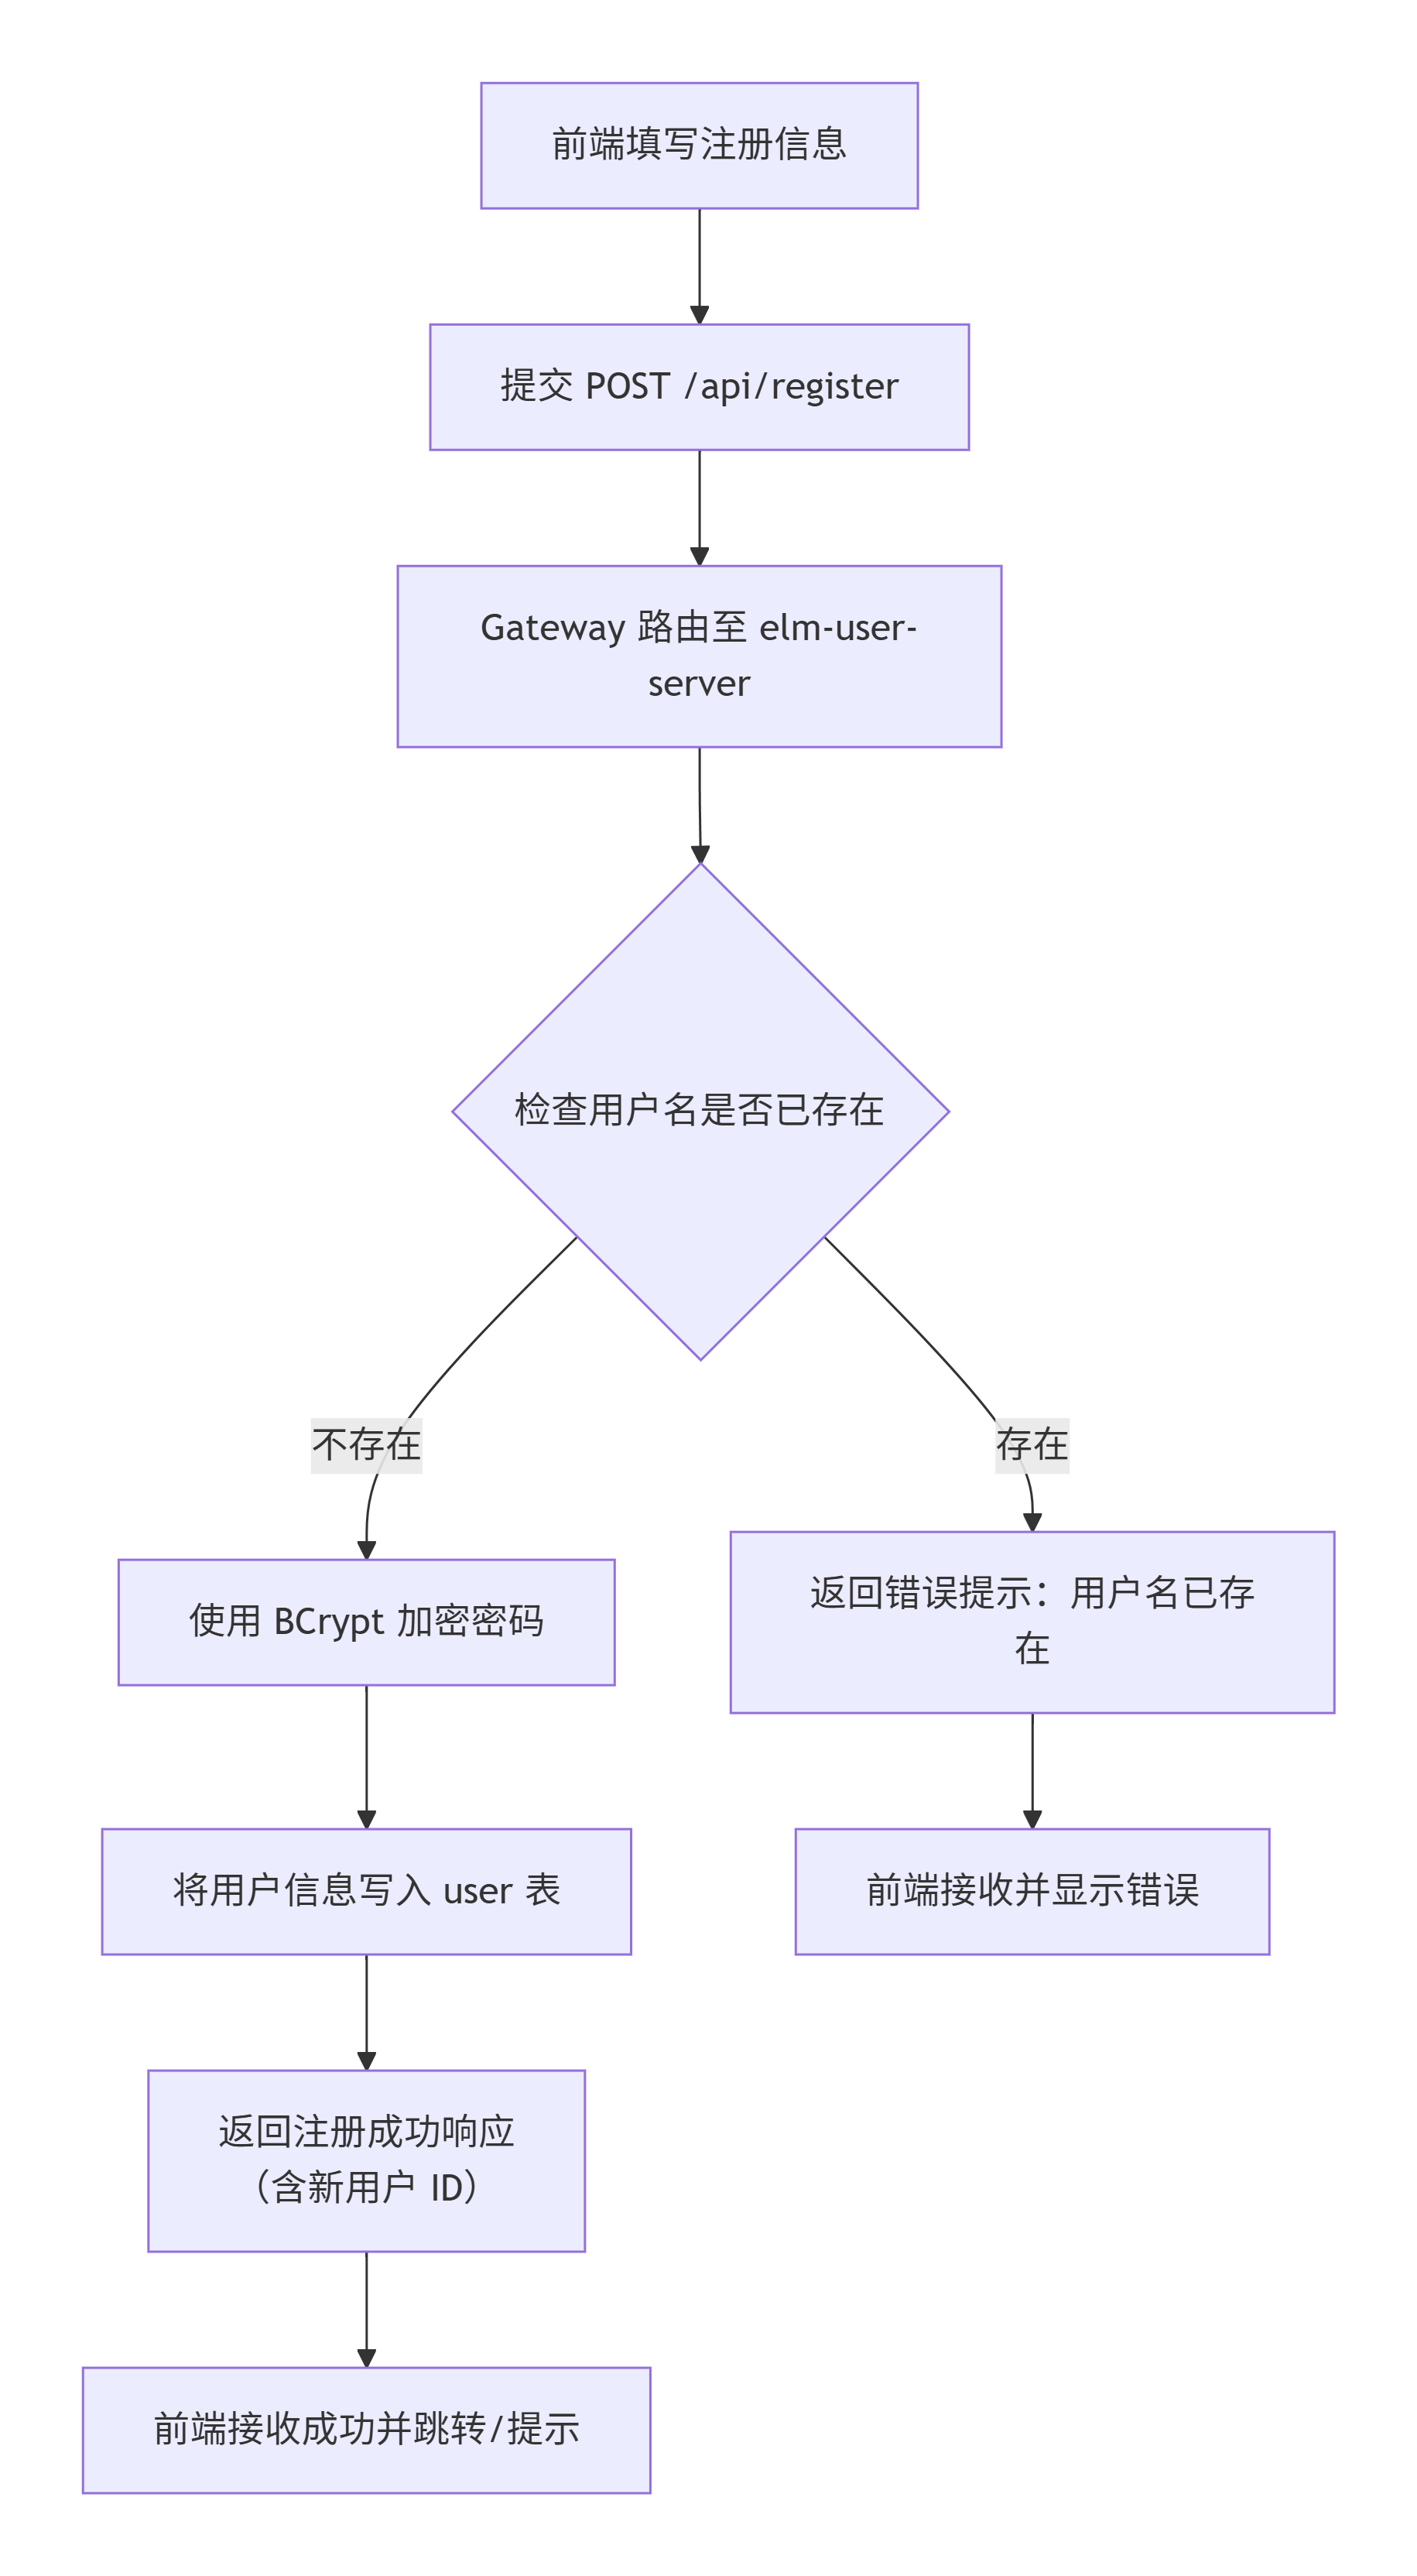
\includegraphics[width=0.75\textwidth,height=0.82\textheight,keepaspectratio]{images/flow-user-register.png}
	\caption{用户注册流程图}
	\label{fig:user-register-flow}
\end{figure}

用户注册流程：用户在前端填写用户名、密码等注册信息后提交POST请求至\verb|/api/register|，请求经Gateway路由至elm-user-server。服务首先检查用户名是否已存在，若不存在则使用BCrypt算法对密码进行哈希加密，将用户信息写入user表，返回注册成功响应（含新用户ID）。若用户名已存在则返回错误提示。

\begin{figure}[H]
	\centering
	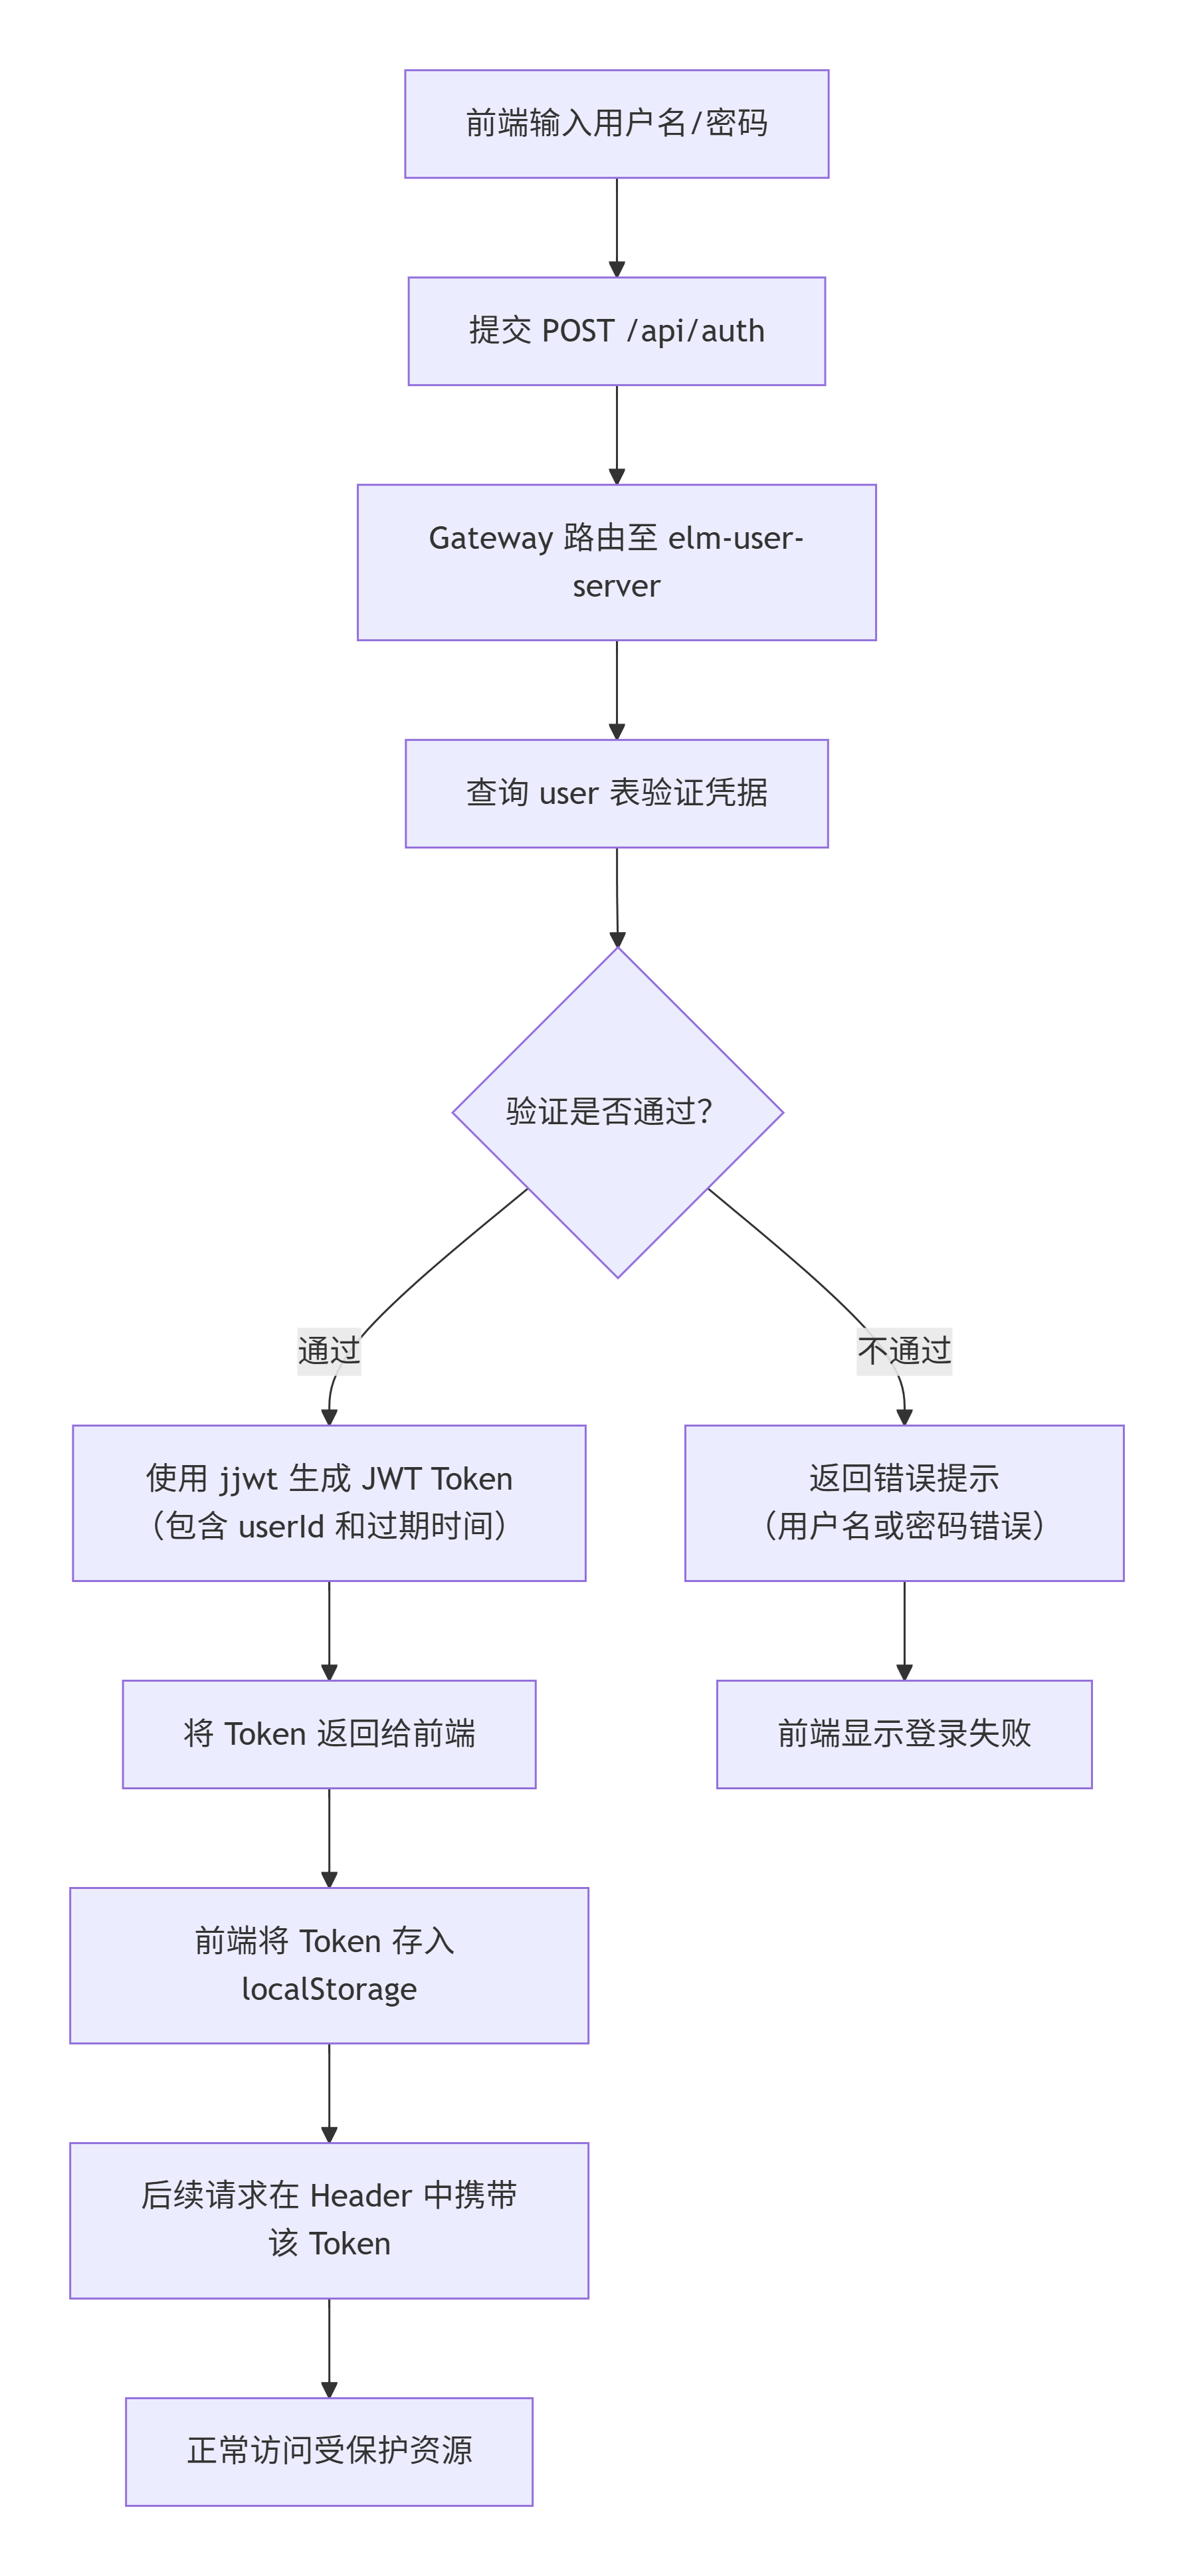
\includegraphics[width=0.75\textwidth,height=0.82\textheight,keepaspectratio]{images/flow-user-login.png}
	\caption{用户登录流程图}
	\label{fig:user-login-flow}
\end{figure}

用户登录流程：用户提交用户名和密码至\verb|/api/auth|，Gateway路由至elm-user-server。服务查询user表验证凭据，验证通过后使用jjwt库生成JWT Token（包含userId和过期时间），将Token返回给前端。前端将Token存入localStorage，后续所有请求均在Header中携带该Token。

\begin{figure}[H]
	\centering
	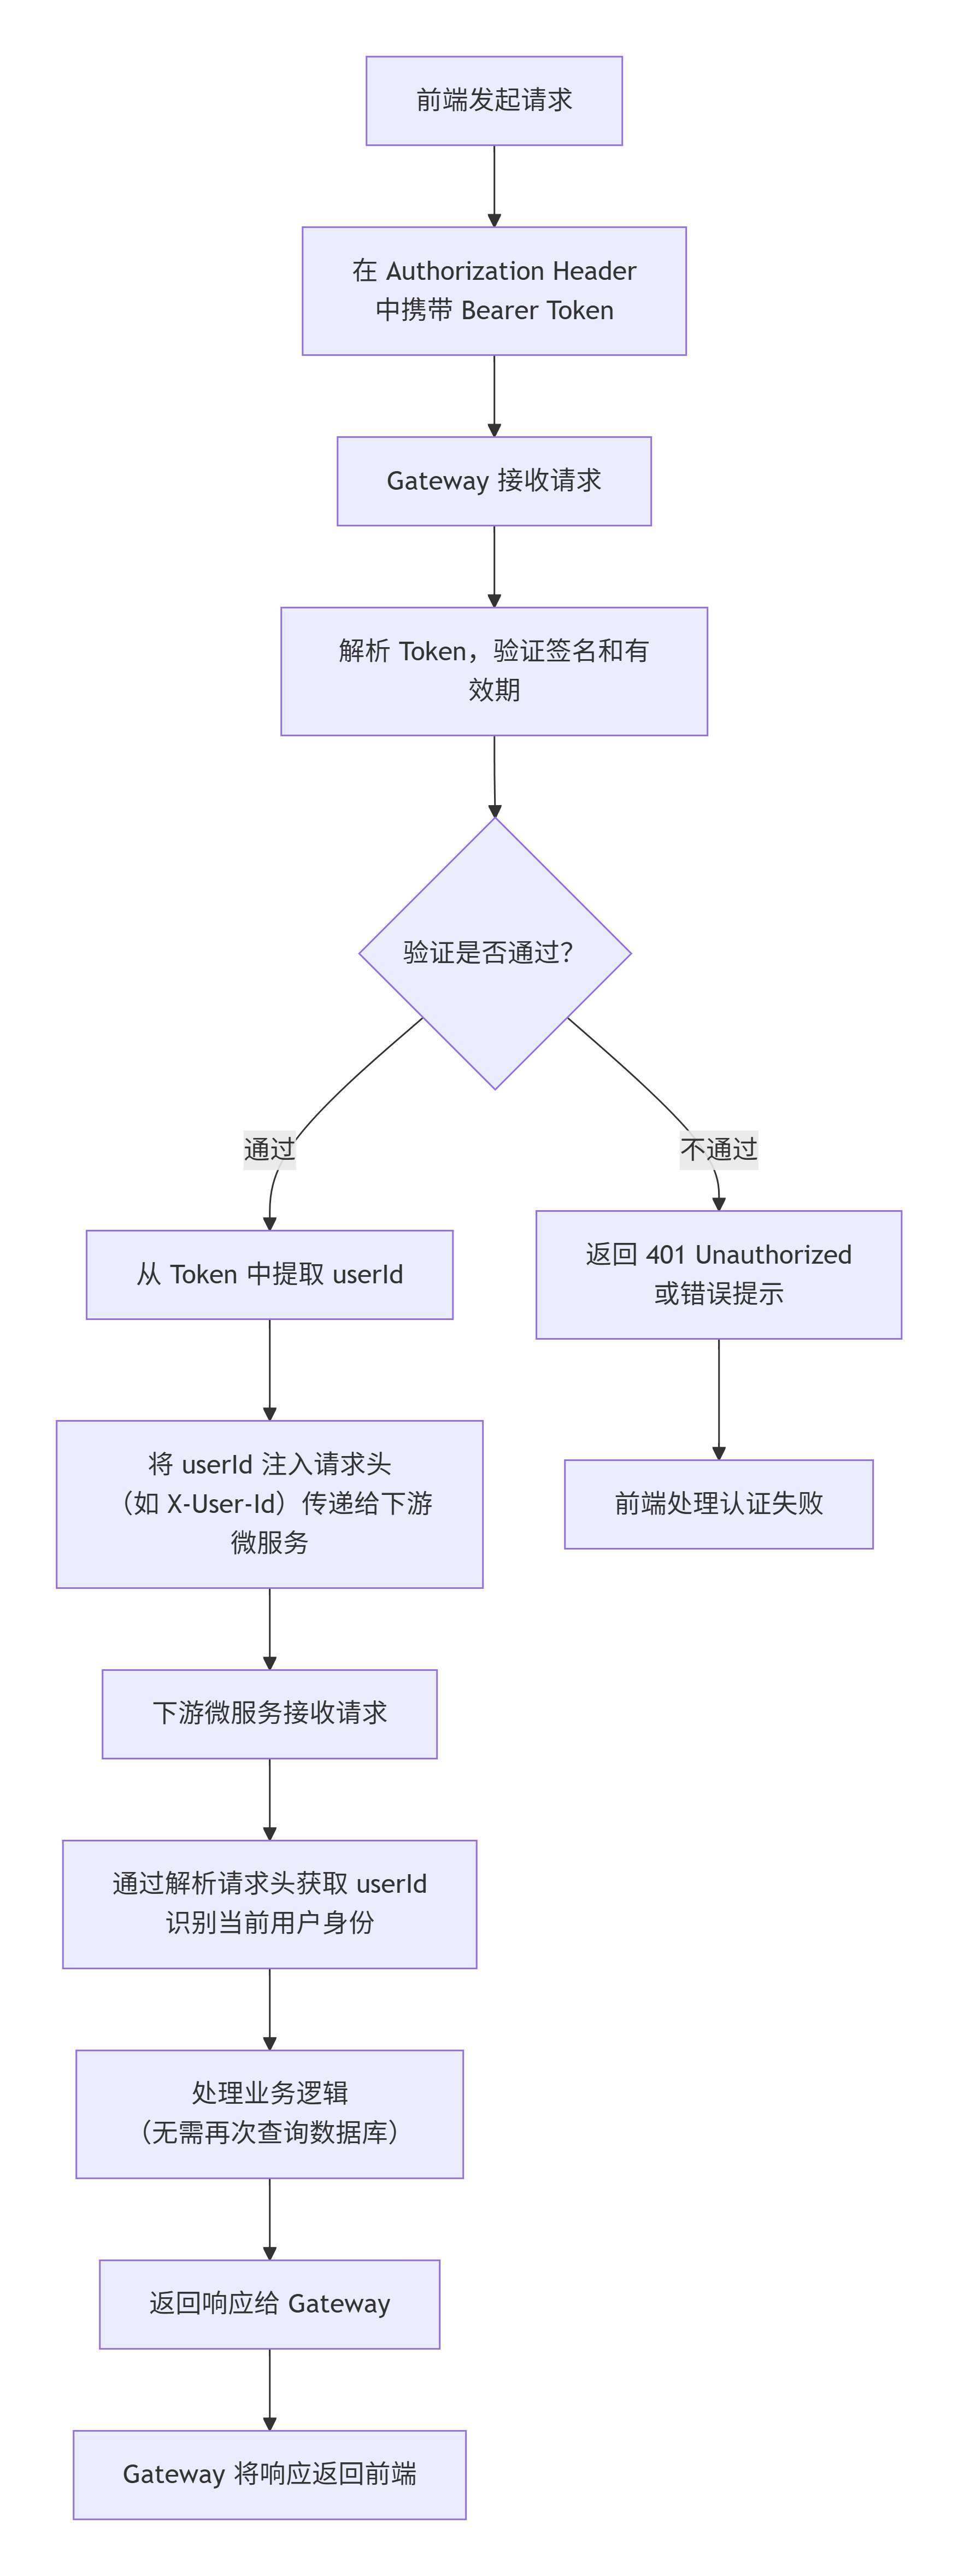
\includegraphics[width=0.75\textwidth,height=0.82\textheight,keepaspectratio]{images/flow-jwt-auth.png}
	\caption{JWT认证流程图}
	\label{fig:jwt-auth-flow}
\end{figure}

JWT认证流程：前端每次请求在Authorization Header中携带Bearer Token，Gateway解析Token验证签名和有效期，从Token中提取userId并注入请求头传递给下游微服务。下游微服务通过解析请求头获取当前用户身份，无需再次查询数据库。

\section{商家微服务 (elm-business-server)}

\begin{longtable}{p{1.5cm}p{2.5cm}p{4.0cm}p{5.5cm}}
	\caption{商家微服务接口一览}\\
	\hline
	\textbf{方法} & \textbf{路径} & \textbf{功能} & \textbf{核心逻辑} \\
	\hline
	\endfirsthead
	GET & /businesses & 获取所有商家 & 列表查询 \\
	GET & /businesses/\{id\} & 按ID获取商家 & 获取商家详情 \\
	GET & /businesses/user/\{id\} & 按用户获取商家 & 获取某用户拥有的商家 \\
	POST & /businesses & 创建商家 & 注册新商家 \\
	PUT & /businesses/\{id\} & 更新商家 & 修改商家信息 \\
	GET & /businesses/order-type/\{id\} & 获取订单类型 & 查询商家订单类型 \\
	POST & /orders & 创建订单 & 创建订单含明细 \\
	GET & /orders/user/\{id\} & 按用户查订单 & 用户订单列表 \\
	GET & /orders/business/\{id\} & 按商家查订单 & 商家订单列表 \\
	GET & /orders/\{id\} & 获取订单详情 & 单个订单 \\
	PUT & /orders/\{id\}/pay & 支付订单 & 状态0→1 \\
	PUT & /orders/\{id\}/deliver & 配送订单 & 状态1→2 \\
	PUT & /orders/\{id\}/checkout & 确认收货 & 状态2→4 \\
	\hline
\end{longtable}

\subsection{商家服务操作流程}

\begin{figure}[H]
	\centering
	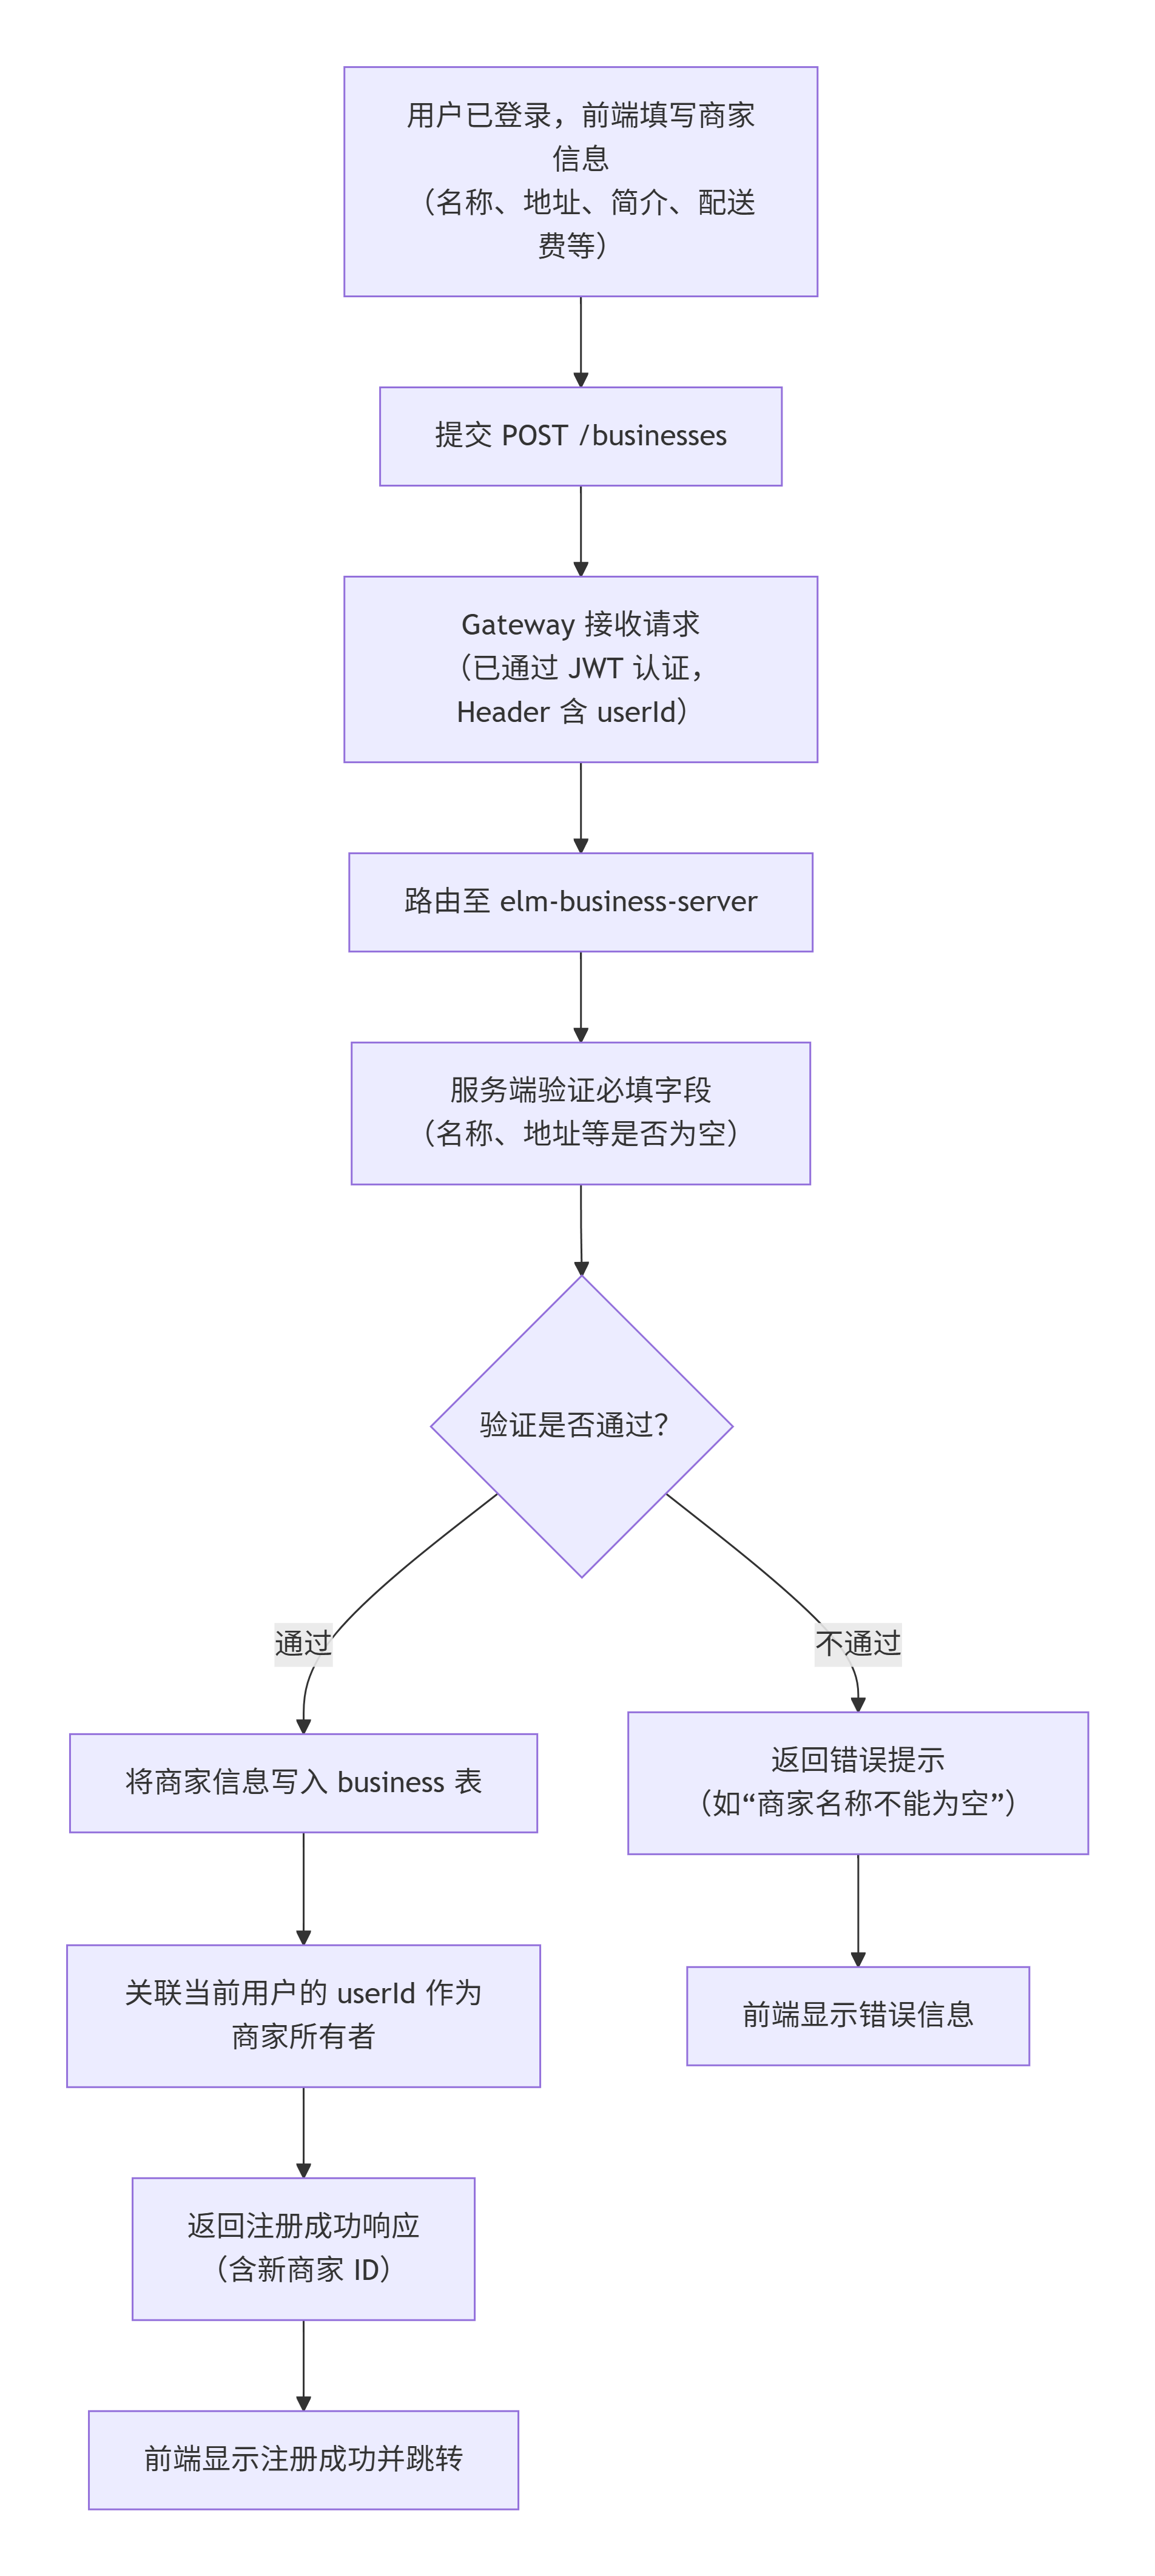
\includegraphics[width=0.75\textwidth,height=0.82\textheight,keepaspectratio]{images/flow-business-register.png}
	\caption{商家注册流程图}
	\label{fig:business-register-flow}
\end{figure}

商家注册流程：用户登录后在前端填写商家信息（名称、地址、简介、配送费等），提交POST请求至\verb|/businesses|。Gateway将请求路由至elm-business-server，服务验证必填字段后将商家信息写入business表，并关联当前用户的userId作为商家所有者。

\begin{figure}[H]
	\centering
	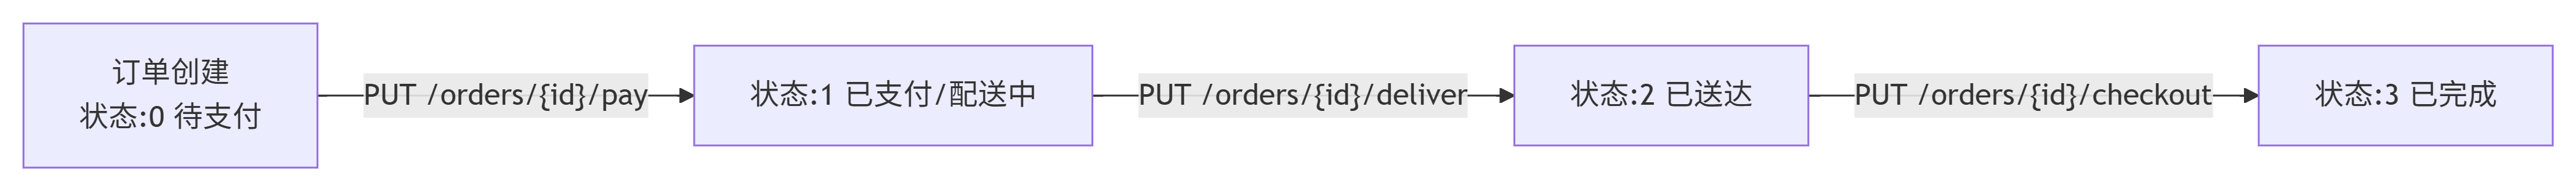
\includegraphics[width=0.75\textwidth,height=0.82\textheight,keepaspectratio]{images/flow-order-state.png}
	\caption{订单状态流转图}
	\label{fig:order-state-flow}
\end{figure}

订单状态流转流程：订单创建后初始状态为0（待支付），商家确认后调用\verb|PUT /orders/{id}/pay|将状态更新为1（已支付/配送中），配送完成后调用\verb|PUT /orders/{id}/deliver|更新为2（已送达），用户确认收货后调用\verb|PUT /orders/{id}/checkout|更新为4（已确认收货）。

\section{食品微服务 (elm-food-server)}

\begin{longtable}{p{1.5cm}p{2.5cm}p{4.0cm}p{5.5cm}}
	\caption{食品微服务接口一览}\\
	\hline
	\textbf{方法} & \textbf{路径} & \textbf{功能} & \textbf{核心逻辑} \\
	\hline
	\endfirsthead
	GET & /foods & 食品列表 & 按businessId筛选，valid=1 \\
	GET & /foods/\{id\} & 按ID查食品 & 获取食品详情 \\
	POST & /foods & 新增食品 & 创建食品，Feign验证商家存在 \\
	PUT & /foods/\{id\} & 更新食品 & 修改食品信息 \\
	DELETE & /foods/\{id\} & 删除食品 & 逻辑删除(valid=0) \\
	\hline
\end{longtable}

\subsection{食品服务操作流程}

\begin{figure}[H]
	\centering
	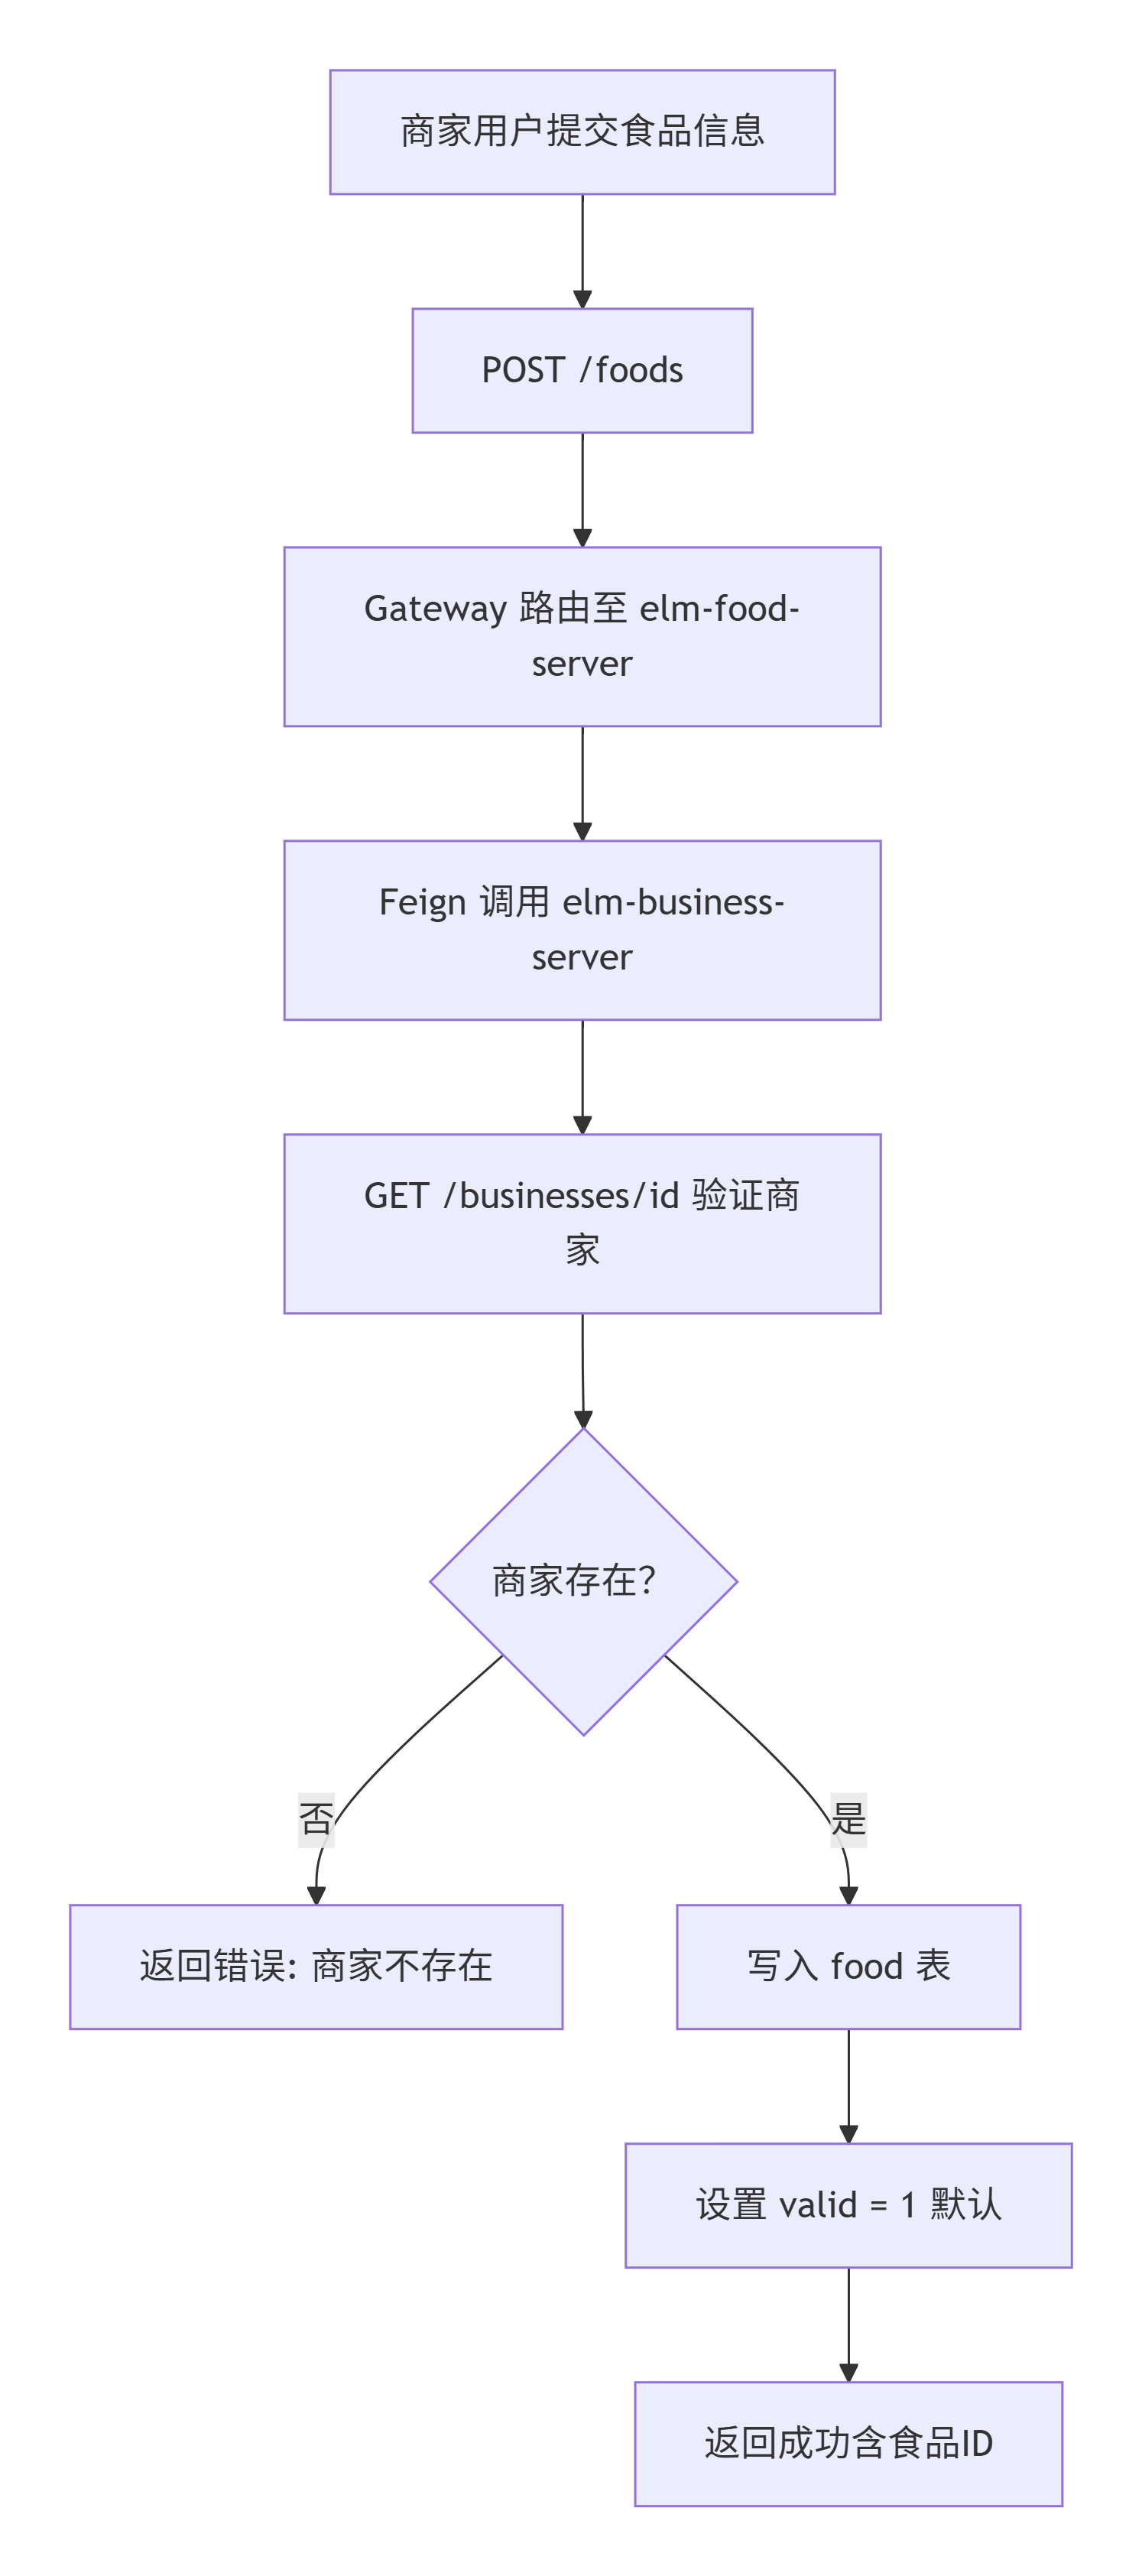
\includegraphics[width=0.75\textwidth,height=0.82\textheight,keepaspectratio]{images/flow-food-manage.png}
	\caption{食品新增流程图}
	\label{fig:food-manage-flow}
\end{figure}

\begin{figure}[H]
	\centering
	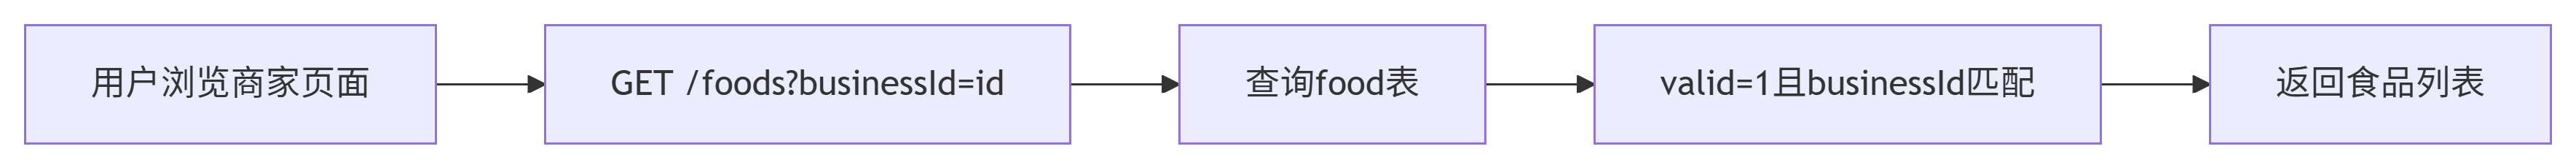
\includegraphics[width=0.75\textwidth,height=0.82\textheight,keepaspectratio]{images/flow-food-query.png}
	\caption{食品查询流程图}
	\label{fig:food-query-flow}
\end{figure}

食品新增流程：商家用户提交食品信息（名称、价格BigDecimal、图片、所属商家ID等）至\verb|POST /foods|。elm-food-server通过Feign客户端调用elm-business-server的\verb|/businesses/{id}|接口验证商家是否存在，验证通过后将食品信息写入food表，valid默认为1。

食品查询流程：用户浏览商家页面时，前端请求\verb|GET /foods?businessId={id}|获取该商家的食品列表。服务查询food表中\verb|valid=1|且\verb|businessId|匹配的记录并返回。

\section{购物车微服务 (elm-cart-server)}

\begin{longtable}{p{1.5cm}p{2.5cm}p{4.0cm}p{5.5cm}}
	\caption{购物车微服务接口一览}\\
	\hline
	\textbf{方法} & \textbf{路径} & \textbf{功能} & \textbf{核心逻辑} \\
	\hline
	\endfirsthead
	GET & /carts/user/\{id\} & 用户购物车 & 用户所有购物车项 \\
	GET & /carts/business/\{id\} & 商家购物车 & 某商家下的购物车 \\
	POST & /carts & 添加商品 & 存在则更新数量，否则新增 \\
	PUT & /carts/\{id\} & 更新数量 & 修改数量 \\
	DELETE & /carts/\{id\} & 删除项目 & 移除购物车项 \\
	\hline
\end{longtable}

\subsection{购物车服务操作流程}

\begin{figure}[H]
	\centering
	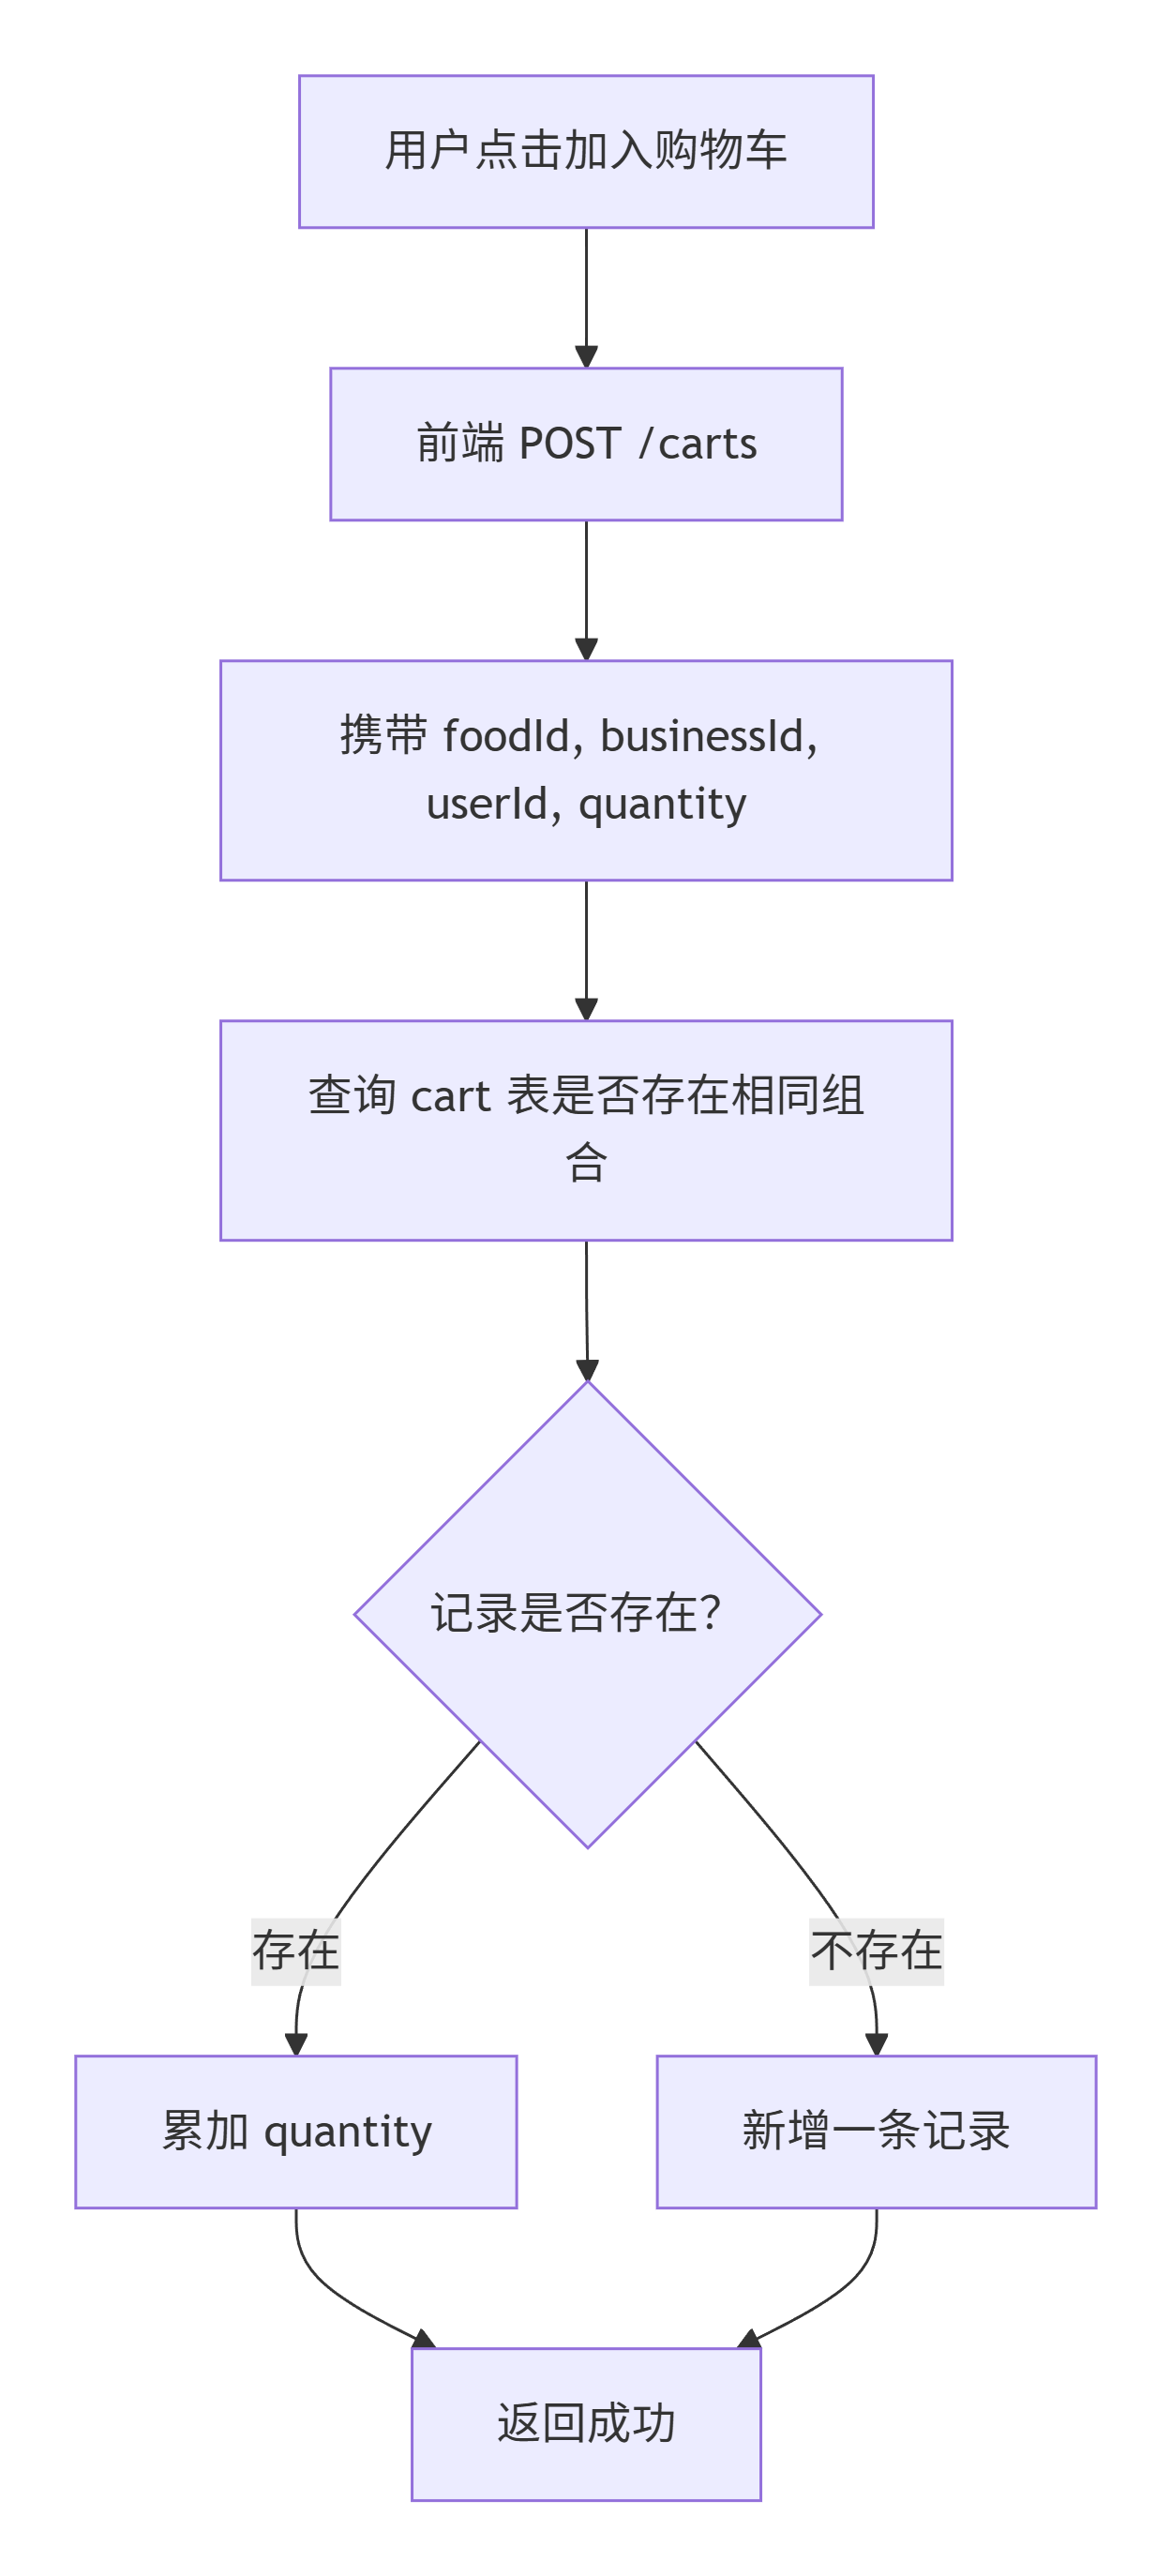
\includegraphics[width=0.75\textwidth,height=0.82\textheight,keepaspectratio]{images/flow-cart-add.png}
	\caption{购物车添加流程图}
	\label{fig:cart-add-flow}
\end{figure}

\begin{figure}[H]
	\centering
	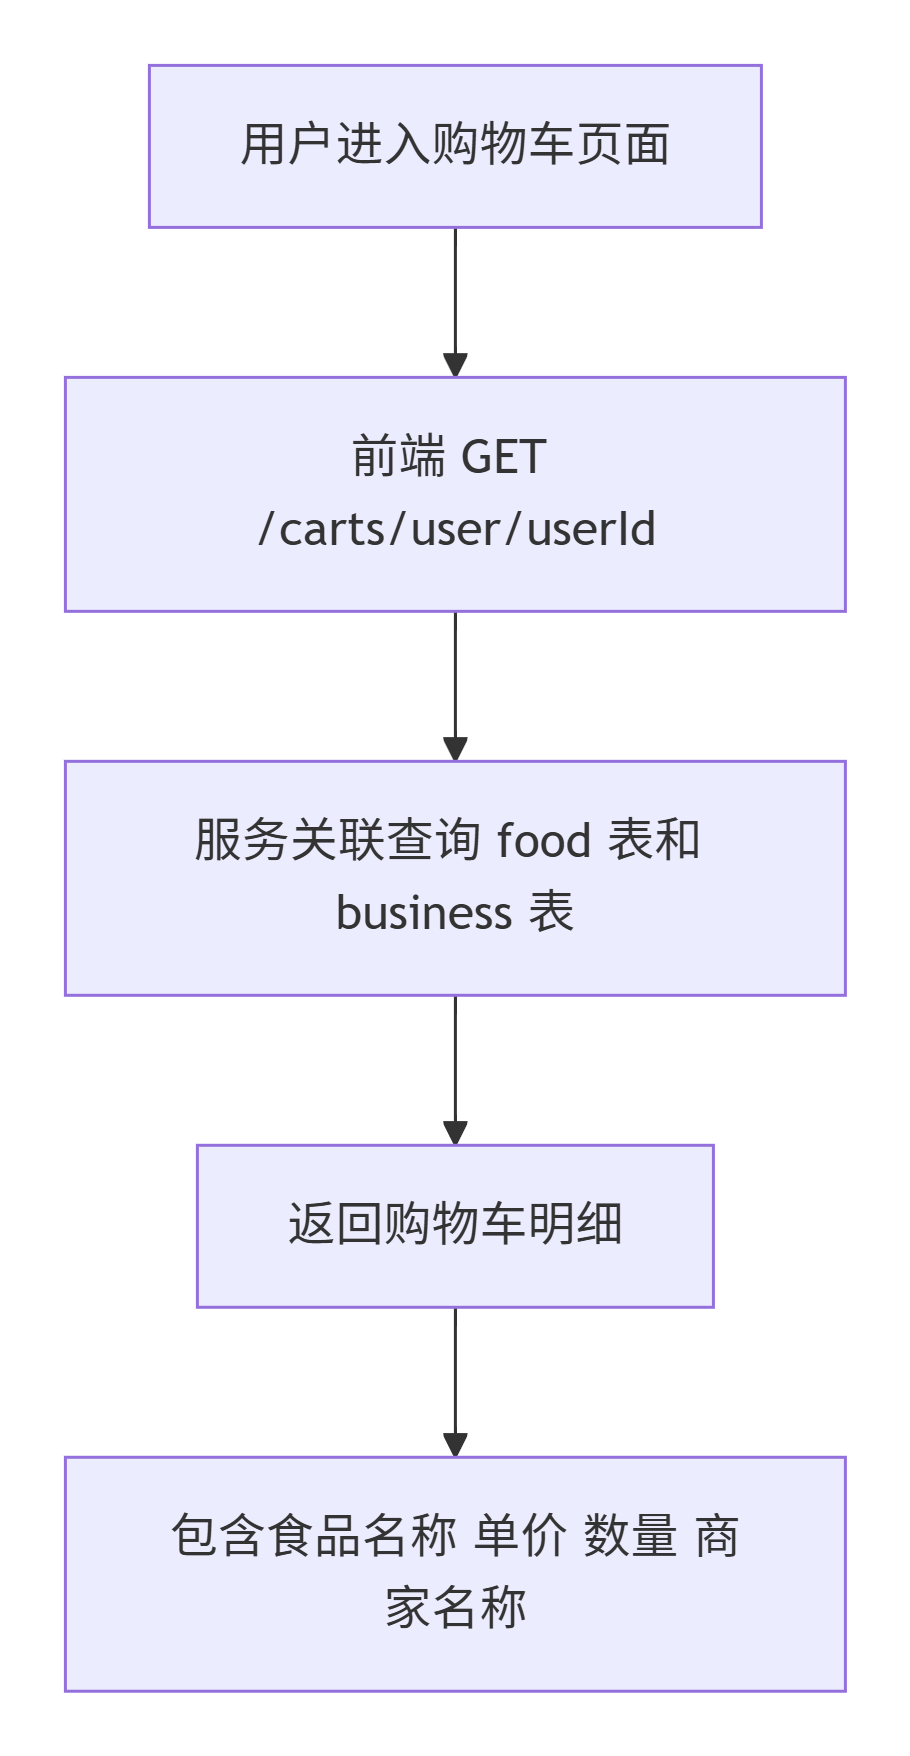
\includegraphics[width=0.75\textwidth,height=0.82\textheight,keepaspectratio]{images/flow-cart-query.png}
	\caption{购物车查询流程图}
	\label{fig:cart-query-flow}
\end{figure}

添加商品流程：用户在食品列表页点击"加入购物车"，前端发送POST请求至\verb|/carts|，携带foodId、businessId、userId和quantity。elm-cart-server查询cart表中是否存在相同的(foodId, businessId, userId)组合——若存在则累加quantity，若不存在则新增一条cart记录。

购物车查询流程：用户进入购物车页面时，前端请求\verb|GET /carts/user/{userId}|获取该用户所有购物车项。服务关联查询food和business表，返回包含食品名称、单价、数量及商家名称的购物车明细。

\section{订单微服务 (elm-order-server)}

\begin{longtable}{p{1.5cm}p{2.8cm}p{4.0cm}p{5.2cm}}
	\caption{订单微服务接口一览}\\
	\hline
	\textbf{方法} & \textbf{路径} & \textbf{功能} & \textbf{核心逻辑} \\
	\hline
	\endfirsthead
	POST & /orders & 创建订单 & 从购物车创建，集成支付和积分 \\
	GET & /orders/user/\{id\} & 用户订单列表 & 用户所有订单 \\
	GET & /orders/business/\{id\} & 商家订单列表 & 商家收到的订单 \\
	GET & /orders/\{id\} & 获取订单详情 & 单个订单含明细 \\
	PUT & /orders/\{id\}/state & 更新订单状态 & 修改订单状态 \\
	POST & /orders/\{id\}/pay/virtual-wallet & 虚拟钱包支付 & 集成钱包转账+积分抵扣，分布式锁保护 \\
	\hline
\end{longtable}

\subsection{订单服务操作流程}

\begin{figure}[H]
	\centering
	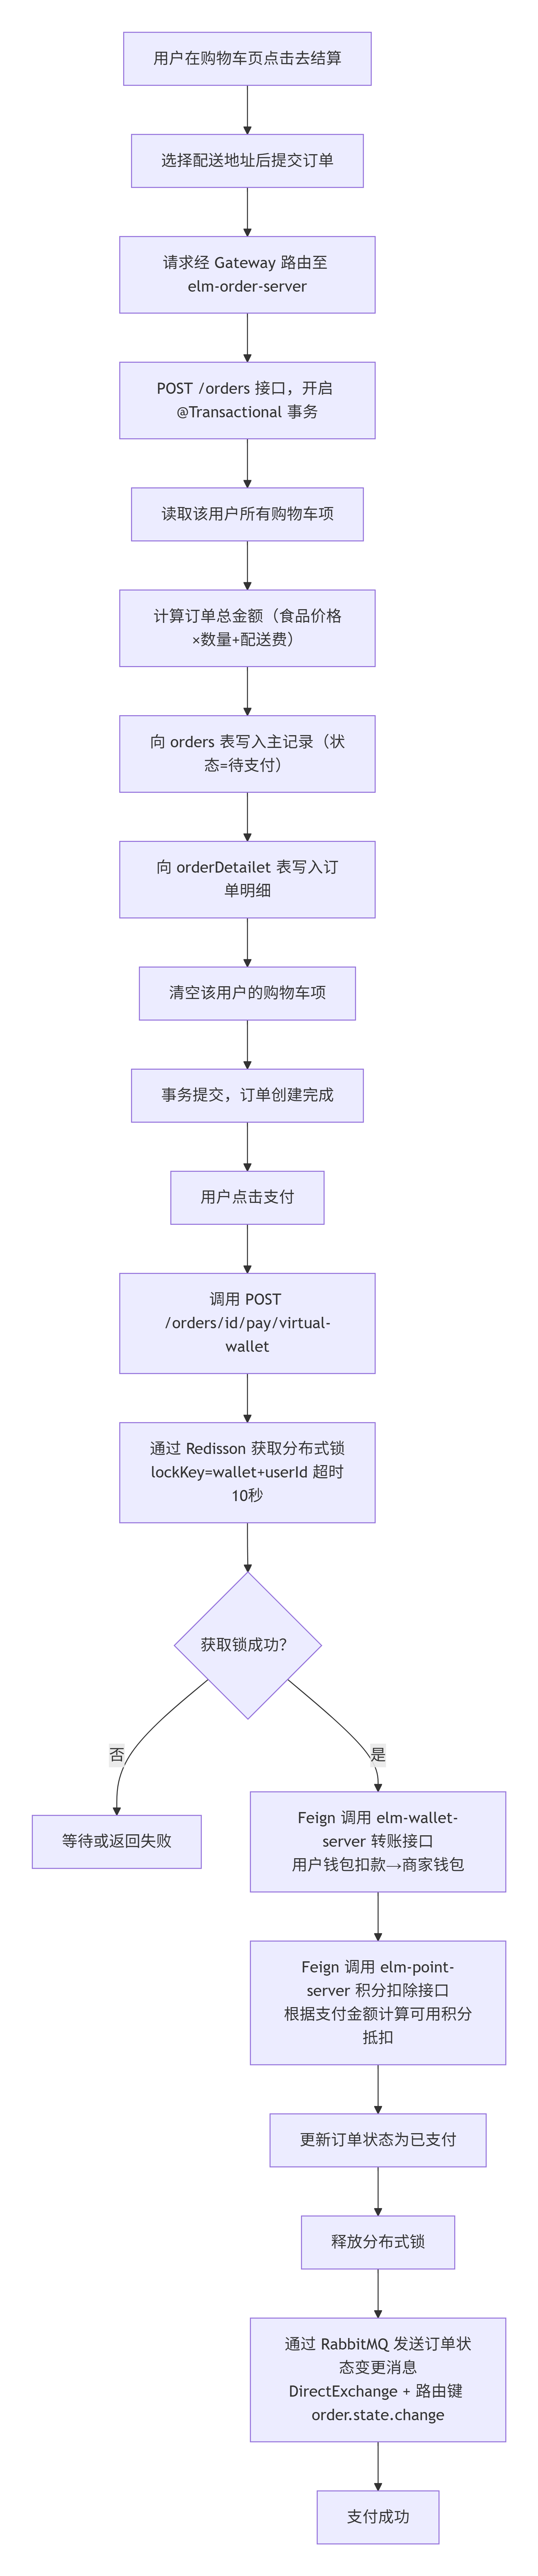
\includegraphics[width=0.75\textwidth,height=0.82\textheight,keepaspectratio]{images/flow-order-create-pay.png}
	\caption{订单创建与支付流程图}
	\label{fig:order-create-pay-flow}
\end{figure}

订单创建与支付流程（核心业务流）：
\begin{enumerate}
	\item 用户在前端购物车页面点击"去结算"，选择配送地址后提交订单
	\item 请求经Gateway路由至elm-order-server的\verb|POST /orders|接口
	\item 服务开启Spring \verb|@Transactional|事务，执行以下步骤：
	\begin{itemize}
		\item 从cart表读取该用户的所有购物车项
		\item 计算订单总金额（食品价格×数量 + 配送费）
		\item 向orders表写入订单主记录（初始状态为待支付）
		\item 向orderDetailet表写入订单明细
		\item 清空该用户的购物车项
	\end{itemize}
	\item 用户点击"支付"，调用\verb|POST /orders/{id}/pay/virtual-wallet|
	\item 服务通过Redisson获取分布式锁（lockKey=wallet+userId，超时10秒）
	\item 在锁保护下执行：
	\begin{itemize}
		\item 通过Feign调用elm-wallet-server的转账接口，从用户钱包扣款至商家钱包
		\item 通过Feign调用elm-point-server的积分扣除接口，根据支付金额计算可用积分抵扣
		\item 更新订单状态为已支付
	\end{itemize}
	\item 释放分布式锁
	\item 通过RabbitMQ发送订单状态变更消息（DirectExchange + 路由键order.state.change）
\end{enumerate}

\section{配送地址微服务 (elm-delivery-server)}

\begin{longtable}{p{1.5cm}p{2.8cm}p{4.0cm}p{5.2cm}}
	\caption{配送地址微服务接口一览}\\
	\hline
	\textbf{方法} & \textbf{路径} & \textbf{功能} & \textbf{核心逻辑} \\
	\hline
	\endfirsthead
	GET & /delivery-addresses/user/\{id\} & 用户地址列表 & 用户所有有效地址 \\
	GET & /delivery-addresses/\{id\} & 按ID查地址 & 单个地址详情 \\
	POST & /delivery-addresses & 新增地址 & 添加配送地址 \\
	PUT & /delivery-addresses/\{id\} & 更新地址 & 修改地址信息 \\
	DELETE & /delivery-addresses/\{id\} & 删除地址 & 逻辑删除(valid=0) \\
	\hline
\end{longtable}

\subsection{配送地址服务操作流程}

\begin{figure}[H]
	\centering
	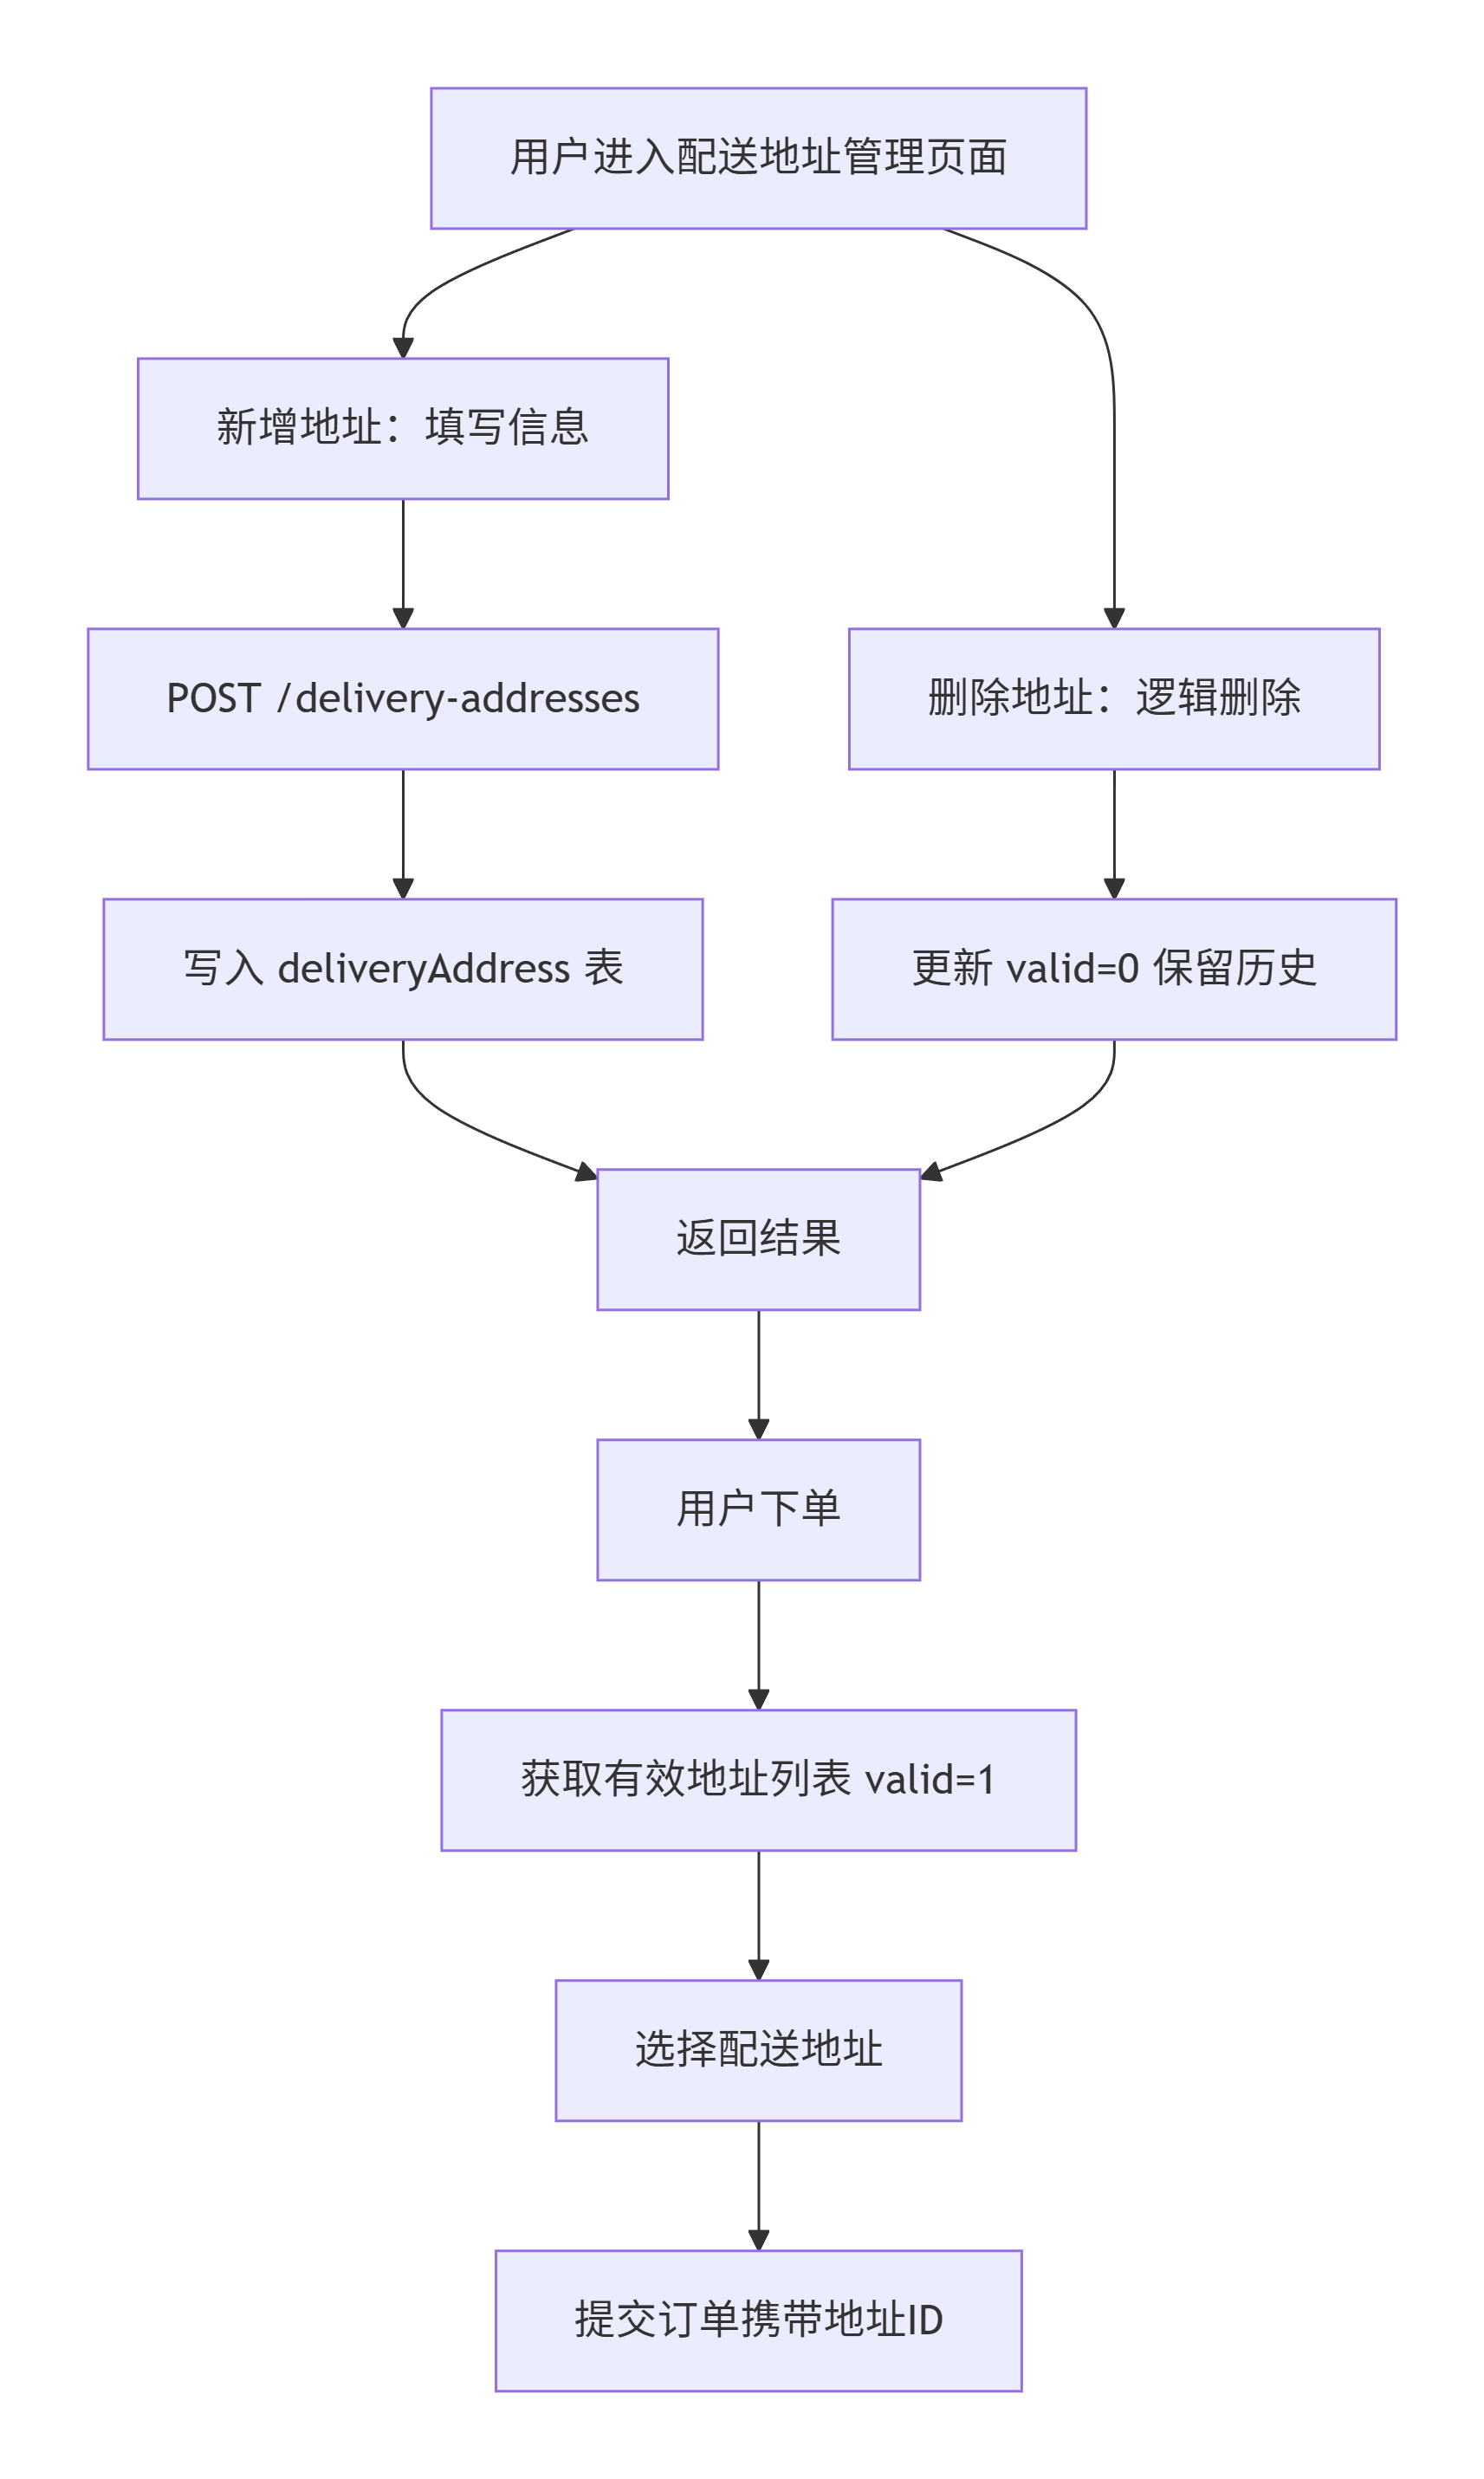
\includegraphics[width=0.75\textwidth,height=0.82\textheight,keepaspectratio]{images/flow-delivery-address.png}
	\caption{配送地址管理流程图}
	\label{fig:delivery-address-flow}
\end{figure}

地址管理流程：用户在下单前可通过配送地址管理页面维护常用地址。新增地址时提交联系人姓名、性别、电话、详细地址至\verb|POST /delivery-addresses|，写入deliveryAddress表。删除地址采用逻辑删除（valid=0），保留历史记录以关联历史订单。下单时用户从有效地址列表中选择一个作为配送地址。

\section{虚拟钱包微服务 (elm-wallet-server)}

\begin{longtable}{p{1.5cm}p{2.8cm}p{4.0cm}p{5.2cm}}
	\caption{虚拟钱包微服务接口一览}\\
	\hline
	\textbf{方法} & \textbf{路径} & \textbf{功能} & \textbf{核心逻辑} \\
	\hline
	\endfirsthead
	GET & /wallet & 获取钱包列表 & 所有钱包 \\
	GET & /wallet/getBalance & 查询余额 & 按userId查询 \\
	POST & /wallet/recharge & 充值 & 增加余额，分布式锁保护 \\
	POST & /wallet/pay & 支付 & 扣减余额 \\
	POST & /wallet/transfer & 转账 & 用户间转账 \\
	POST & /wallet/repayOverdraft & 还款 & 归还透支金额 \\
	POST & /vip/purchase & 购买VIP & 99元/299元VIP卡，设置信用额度2000 \\
	\hline
\end{longtable}

\subsection{钱包服务操作流程}

\begin{figure}[H]
	\centering
	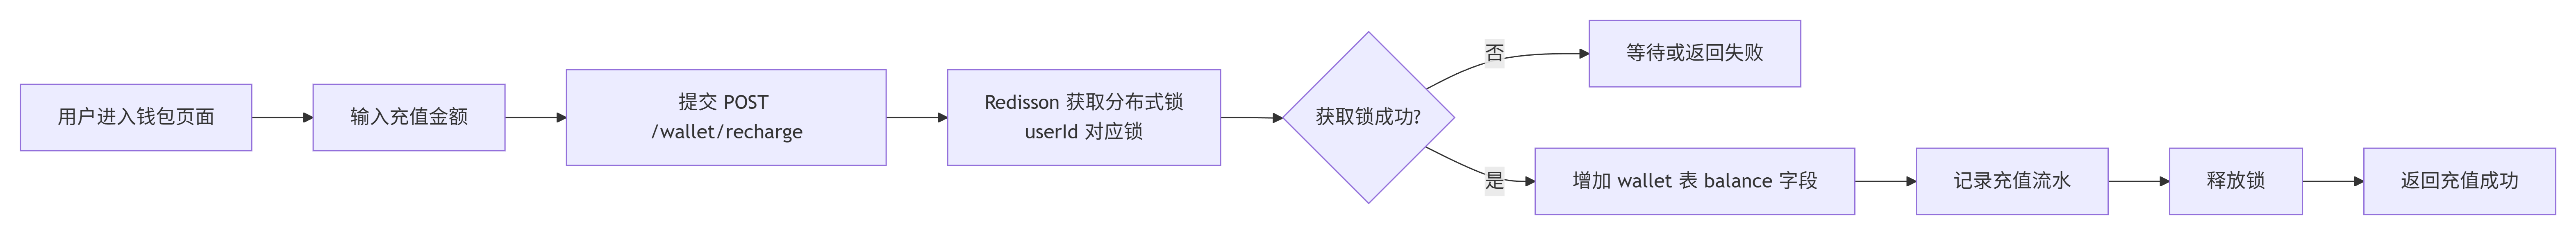
\includegraphics[width=0.75\textwidth,height=0.82\textheight,keepaspectratio]{images/flow-wallet-recharge.png}
	\caption{钱包充值流程图}
	\label{fig:wallet-recharge-flow}
\end{figure}

钱包充值流程：用户进入钱包页面，输入充值金额，提交\verb|POST /wallet/recharge|。服务通过Redisson获取userId对应的分布式锁，在锁保护下增加wallet表中的balance字段，记录充值流水。

\begin{figure}[H]
	\centering
	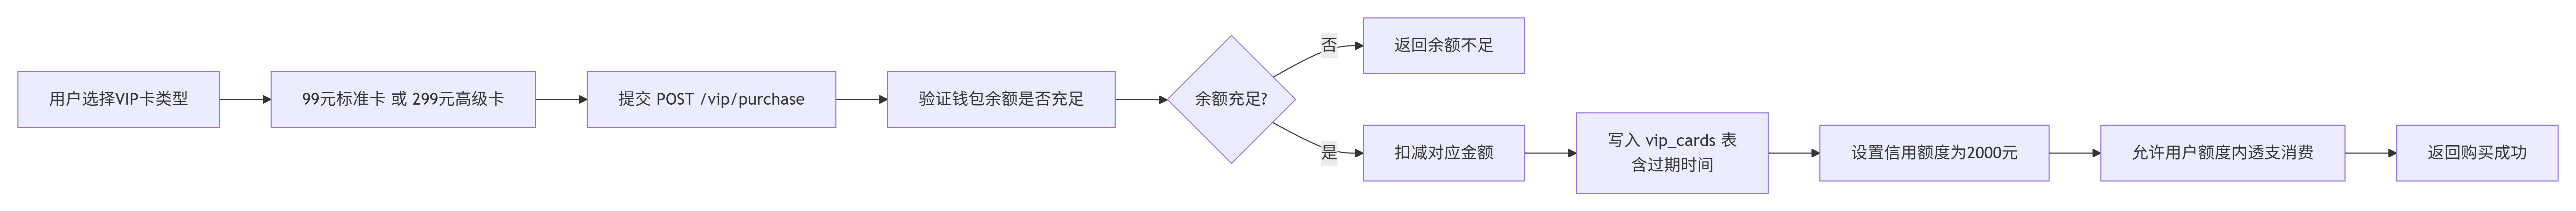
\includegraphics[width=0.75\textwidth,height=0.82\textheight,keepaspectratio]{images/flow-vip-purchase.png}
	\caption{VIP购买流程图}
	\label{fig:vip-purchase-flow}
\end{figure}

VIP购买流程：用户选择VIP卡类型（99元标准卡或299元高级卡），调用\verb|POST /vip/purchase|。服务验证钱包余额充足后扣减对应金额，在vip\_cards表中写入购买记录（含过期时间），同时将信用额度设置为2000元，允许用户在一定额度内透支消费。

\section{积分微服务 (elm-point-server)}

\begin{longtable}{p{1.5cm}p{2.8cm}p{4.0cm}p{5.2cm}}
	\caption{积分微服务接口一览}\\
	\hline
	\textbf{方法} & \textbf{路径} & \textbf{功能} & \textbf{核心逻辑} \\
	\hline
	\endfirsthead
	GET & /integral/available & 查询可用积分 & 用户可用积分余额 \\
	GET & /integral/details & 积分明细 & 积分收支明细 \\
	GET & /integral/statistics & 积分统计 & 总计/可用/已用/过期 \\
	POST & /integral/add & 增加积分 & 管理员发放/活动奖励 \\
	POST & /integral/consume & 消费积分 & 积分消费 \\
	POST & /integral/signIn & 签到 & 每日签到奖励，连续天数越多奖励越多 \\
	POST & /integral/comment & 发表评论 & 评论获积分 \\
	POST & /integral/exchange & 积分兑换 & 积分兑换商品 \\
	GET & /points/balance & 积分余额 & 基础积分余额（Feign用） \\
	POST & /points/earn & 积分赚取 & 基础积分增加（Feign用） \\
	POST & /points/deduct & 积分扣除 & 基础积分扣减（Feign用） \\
	POST/GET & /promotion-day/** & 红包配置 & 红包雨活动管理 \\
	\hline
\end{longtable}

\subsection{积分服务操作流程}

\begin{figure}[H]
	\centering
	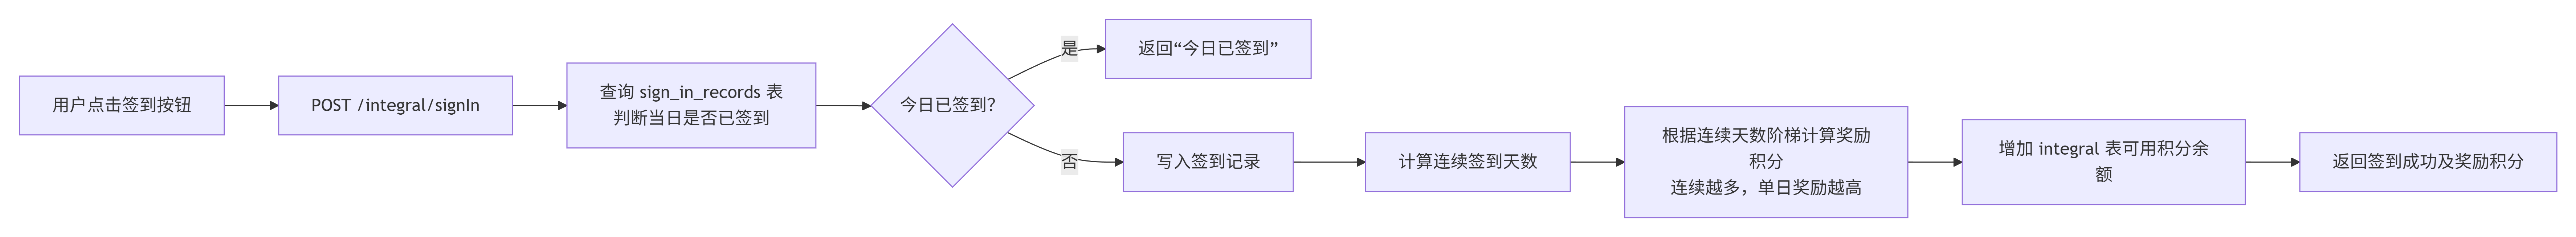
\includegraphics[width=0.75\textwidth,height=0.82\textheight,keepaspectratio]{images/flow-signin.png}
	\caption{每日签到流程图}
	\label{fig:signin-flow}
\end{figure}

每日签到流程：用户每日在前端点击签到按钮，调用\verb|POST /integral/signIn|。服务查询sign\_in\_records表判断当日是否已签到。若未签到则写入签到记录，计算连续签到天数，根据连续天数阶梯计算奖励积分（连续天数越多，单日奖励越高），增加integral表中可用积分余额。

\begin{figure}[H]
	\centering
	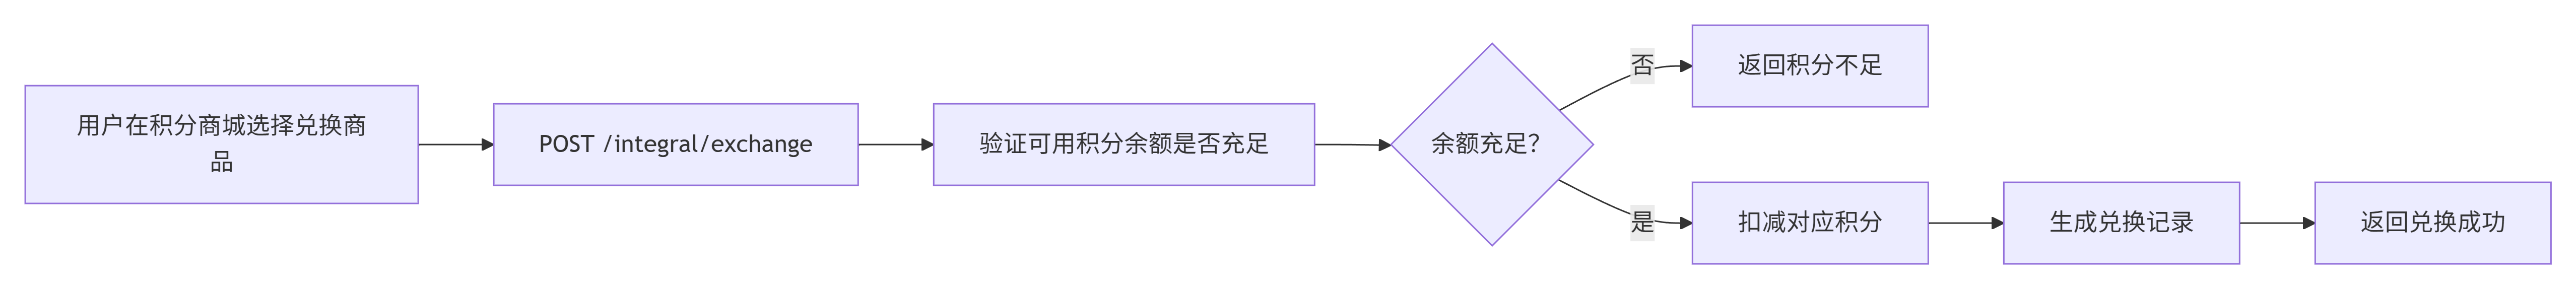
\includegraphics[width=0.75\textwidth,height=0.82\textheight,keepaspectratio]{images/flow-points-exchange.png}
	\caption{积分兑换流程图}
	\label{fig:points-exchange-flow}
\end{figure}

积分兑换流程：用户在积分商城选择兑换商品，调用\verb|POST /integral/exchange|。服务验证可用积分余额是否充足，验证通过后扣减对应积分并生成兑换记录。

\begin{figure}[H]
	\centering
	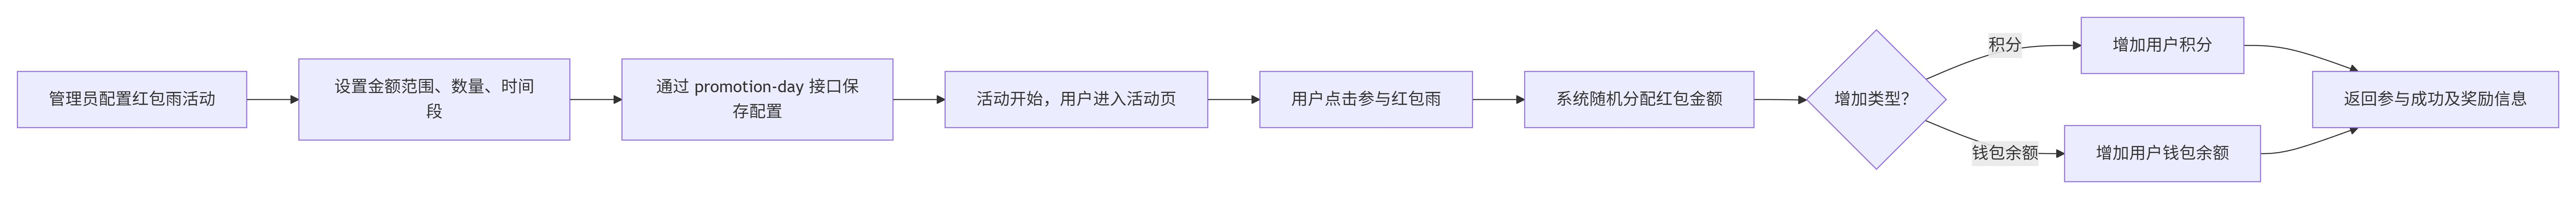
\includegraphics[width=0.75\textwidth,height=0.82\textheight,keepaspectratio]{images/flow-promotion.png}
	\caption{红包雨活动流程图}
	\label{fig:promotion-flow}
\end{figure}

红包雨活动流程：管理员通过promotion-day接口配置红包雨活动（设置红包金额范围、数量、活动时间段）。活动期间用户在前端参与红包雨，系统随机分配红包金额并增加用户积分或钱包余额。

\section{数据库表结构汇总}

系统使用elm2数据库（utf8mb4字符集），核心表包括：

\begin{itemize}
	\item \textbf{user}：userId（主键）、password、userName、userSex、userImg、delTag、userType
	\item \textbf{business}：businessId（自增主键）、businessName、businessAddress、businessExplain、businessImg、orderTypeId、starPrice（DECIMAL）、deliveryPrice（DECIMAL）、remarks、userId
	\item \textbf{food}：foodId（自增主键）、foodName、foodExplain、foodImg、foodPrice（DECIMAL）、businessId、remarks、valid
	\item \textbf{cart}：cartId（自增主键）、foodId、businessId、userId、quantity，唯一约束(foodId,businessId,userId)
	\item \textbf{deliveryAddress}：daId（自增主键）、contactName、contactSex、contactTel、address、userId、valid
	\item \textbf{orders}：orderId（自增主键）、userId、businessId、orderDate、orderTotal（DECIMAL）、daId、orderState
	\item \textbf{orderDetailet}：odId（自增主键）、orderId、foodId、quantity
	\item \textbf{VirtualWallet}：walletId（自增主键）、userId（UNIQUE）、balance（DECIMAL）、creditLimit、usedCreditLimit、lastInterestTime
	\item \textbf{integral}：id（自增主键）、user\_id（VARCHAR(50)）、amount、type、status、channel、expire\_time、business\_id、description、remaining\_amount
	\item \textbf{sign\_in\_records}：id（自增主键）、user\_id（VARCHAR(50)）、sign\_date、consecutive\_days、points\_awarded
	\item \textbf{vip\_cards}：cardId（自增主键）、userId、cardType、price、purchaseTime、expiryTime、status
	\item \textbf{overdraft\_records}：recordId（自增主键）、walletId、overdraftAmount、repaidAmount、dailyInterestRate、status
\end{itemize}
   % 所有功能设计汇总
	% !Mode:: "TeX:UTF-8"

\chapter{前端页面展示}

本项目前端基于Vue.js 3框架和Element Plus组件库构建，采用单页面应用（SPA）架构，实现了响应式布局和组件化开发。以下按功能模块展示各核心页面。

\section{用户认证模块}

\subsection{登录页面}

\begin{figure}[H]
	\centering
	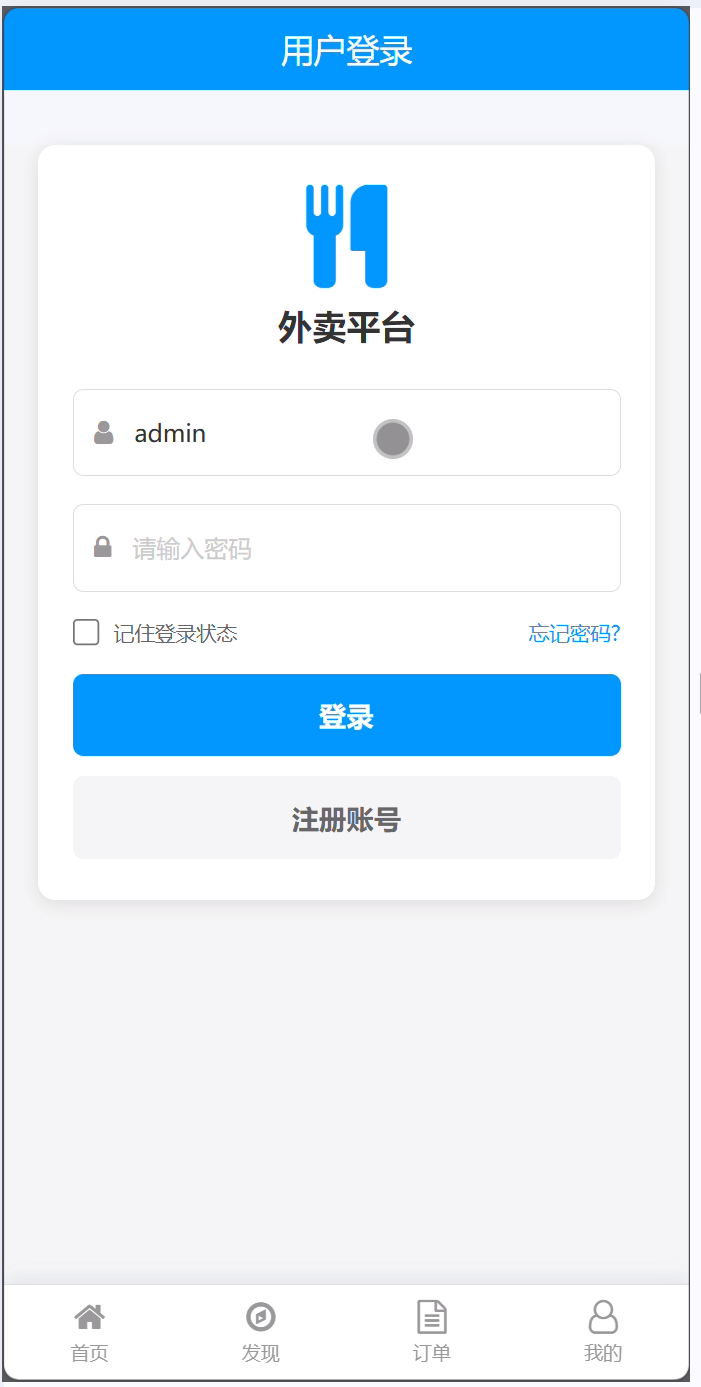
\includegraphics[width=0.75\textwidth,height=0.82\textheight,keepaspectratio]{images/page-login.png}
	\caption{登录页面}
	\label{fig:login-page}
\end{figure}

登录页面（Login.vue）提供用户名和密码输入表单，支持表单验证（必填项检查）。用户提交登录请求后，前端调用\verb|POST /api/auth|获取JWT Token，将Token存入localStorage并跳转至首页。页面顶部展示项目Logo和标题"ELM外卖平台"，底部提供"去注册"的导航链接。

\subsection{注册页面}

\begin{figure}[H]
	\centering
	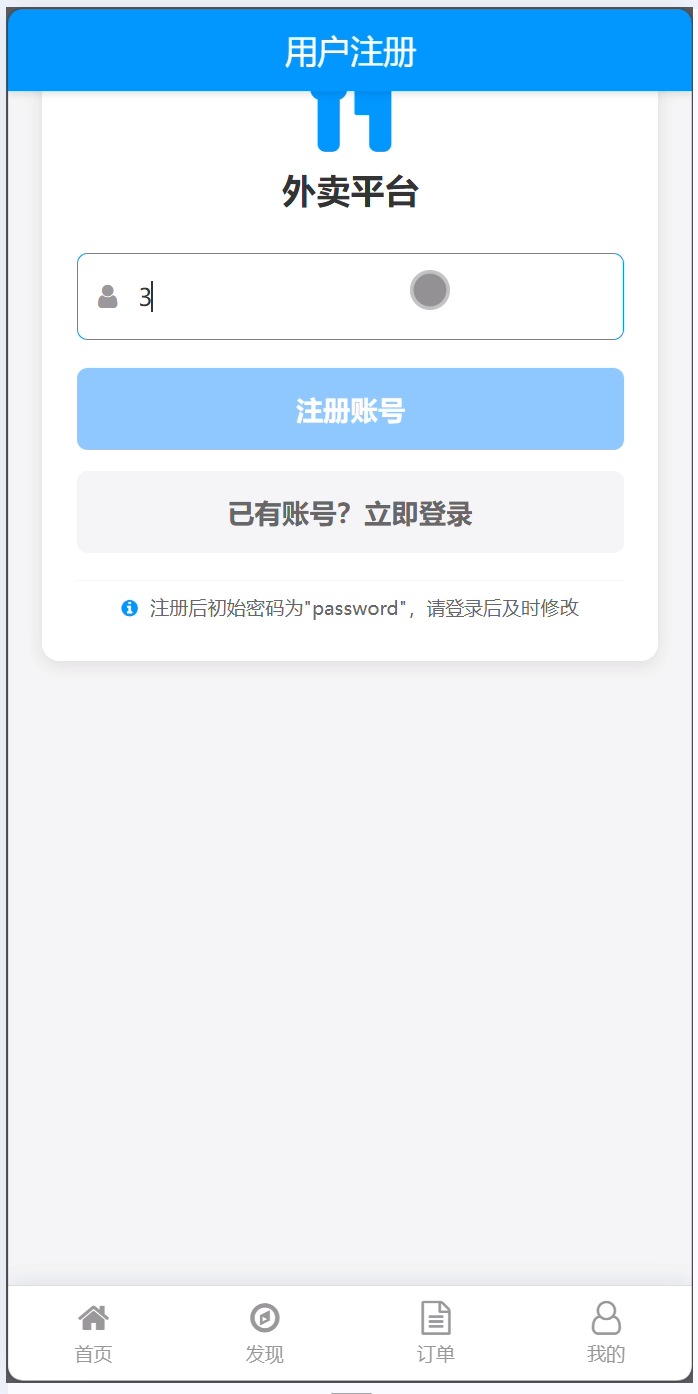
\includegraphics[width=0.75\textwidth,height=0.82\textheight,keepaspectratio]{images/page-register.png}
	\caption{注册页面}
	\label{fig:register-page}
\end{figure}

注册页面（Register.vue）提供用户名、密码、确认密码、用户性别等注册信息表单。前端对密码和确认密码进行一致性校验，对用户名长度进行合法性检查。提交注册请求至\verb|POST /api/register|，注册成功后自动跳转至登录页面。


\section{首页与导航}

\subsection{首页}

\begin{figure}[H]
	\centering
	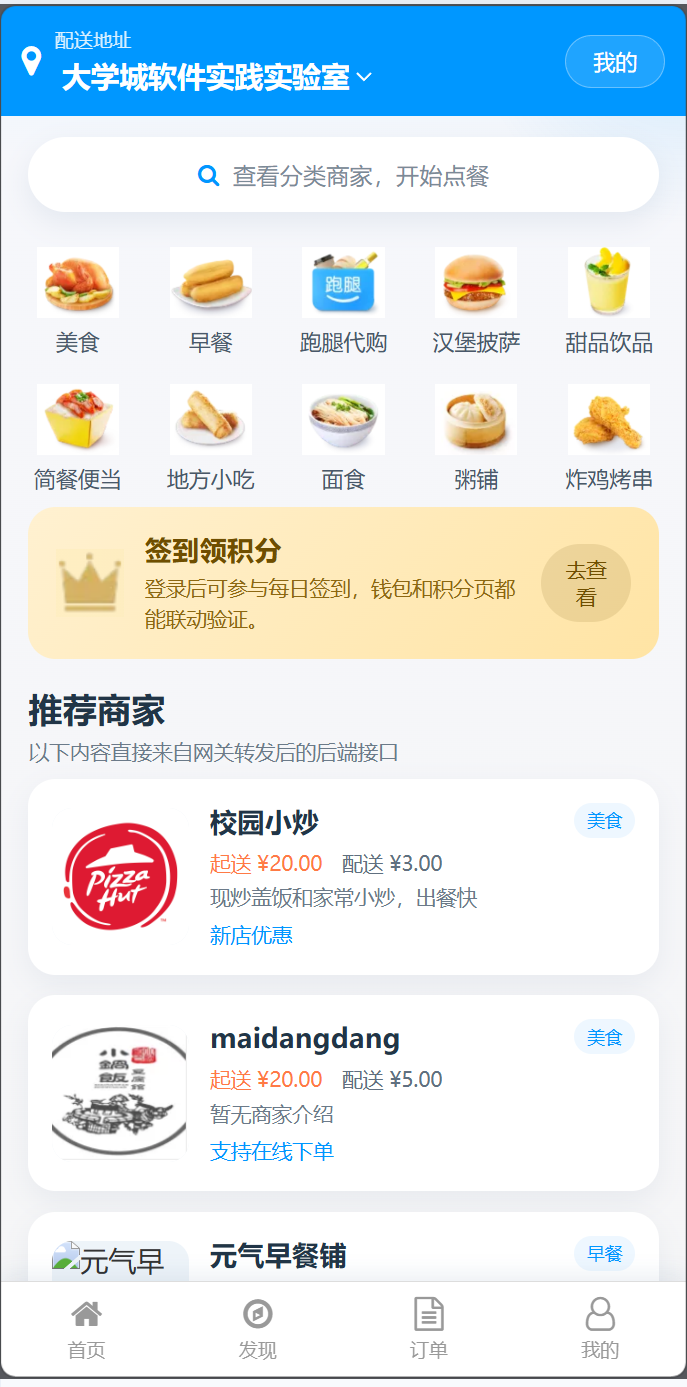
\includegraphics[width=0.75\textwidth,height=0.82\textheight,keepaspectratio]{images/page-index.png}
	\caption{首页}
	\label{fig:index-page}
\end{figure}

首页（Index.vue）作为用户登录后的主入口，展示顶部导航栏（包含商家列表、订单、购物车、钱包、积分等入口），中间区域展示轮播Banner和推荐商家列表，底部展示版权信息。导航栏根据用户登录状态动态显示不同菜单项。

\subsection{用户首页}

\begin{figure}[H]
	\centering
	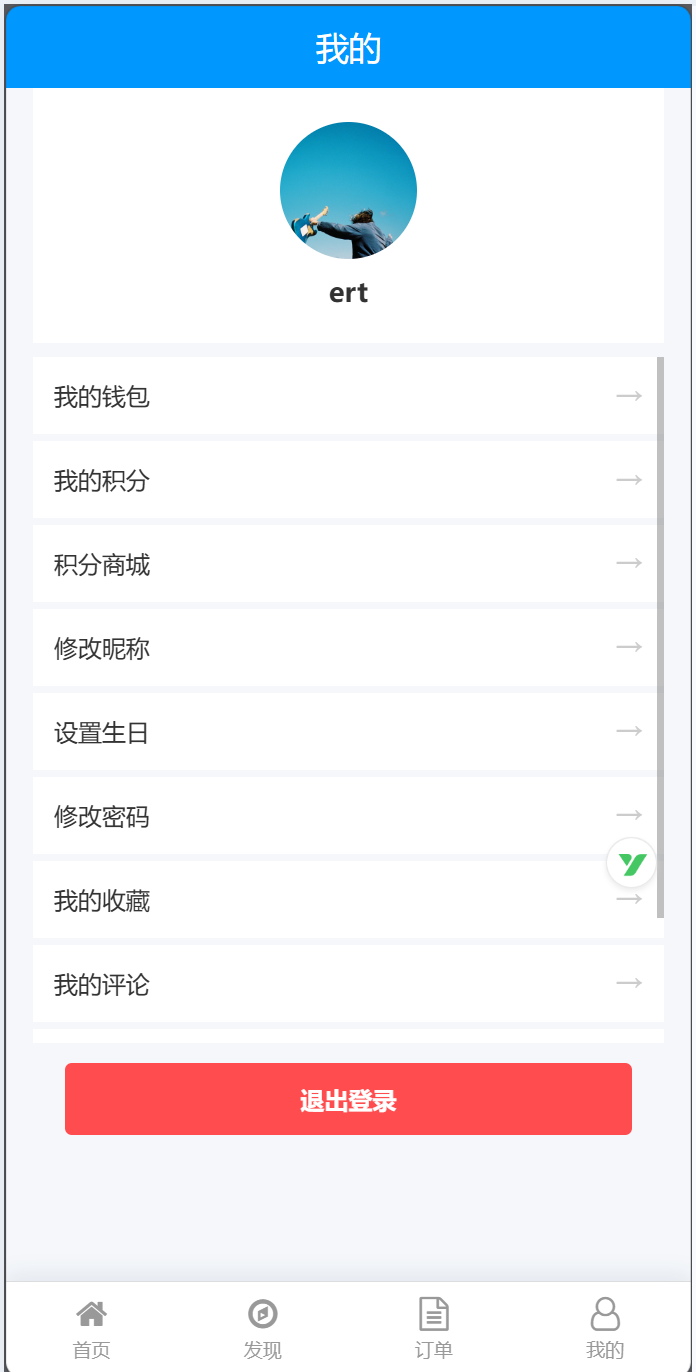
\includegraphics[width=0.75\textwidth,height=0.82\textheight,keepaspectratio]{images/page-user-home.png}
	\caption{用户首页}
	\label{fig:user-home-page}
\end{figure}

用户首页（UserHome.vue）展示用户个人信息概览，包括用户名、头像、会员等级，以及快捷入口卡片（我的订单、钱包余额、可用积分、VIP状态等）。

\section{商家模块}

\subsection{商家列表页面}

\begin{figure}[H]
	\centering
	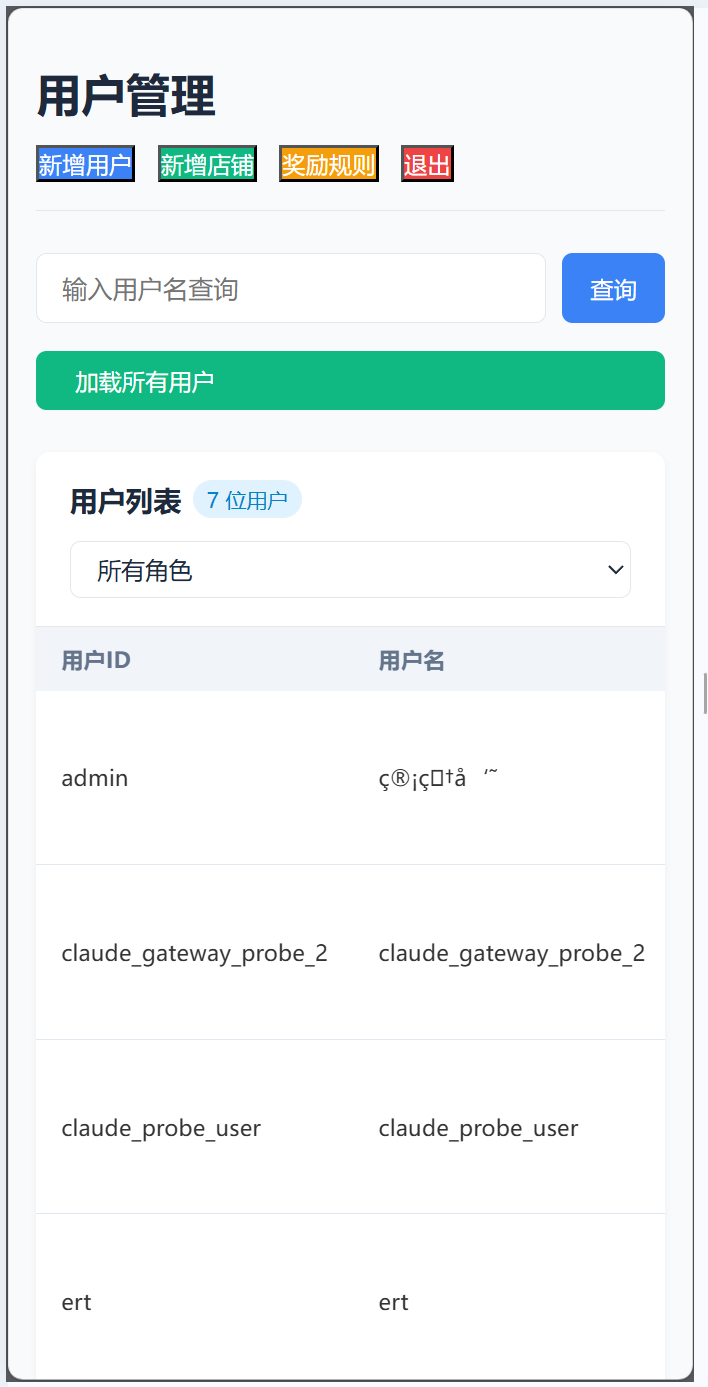
\includegraphics[width=0.75\textwidth,height=0.82\textheight,keepaspectratio]{images/page-business-list.png}
	\caption{商家列表页面}
	\label{fig:business-list-page}
\end{figure}

商家列表页面（BusinessList.vue）以卡片列表形式展示所有注册商家，每张卡片包含商家名称、商家图片、起送价（starPrice）、配送费（deliveryPrice）、商家简介和评分信息。支持按商家名称搜索和按配送费/起送价排序。点击商家卡片进入商家详情页。

\subsection{商家详情页面}

\begin{figure}[H]
	\centering
	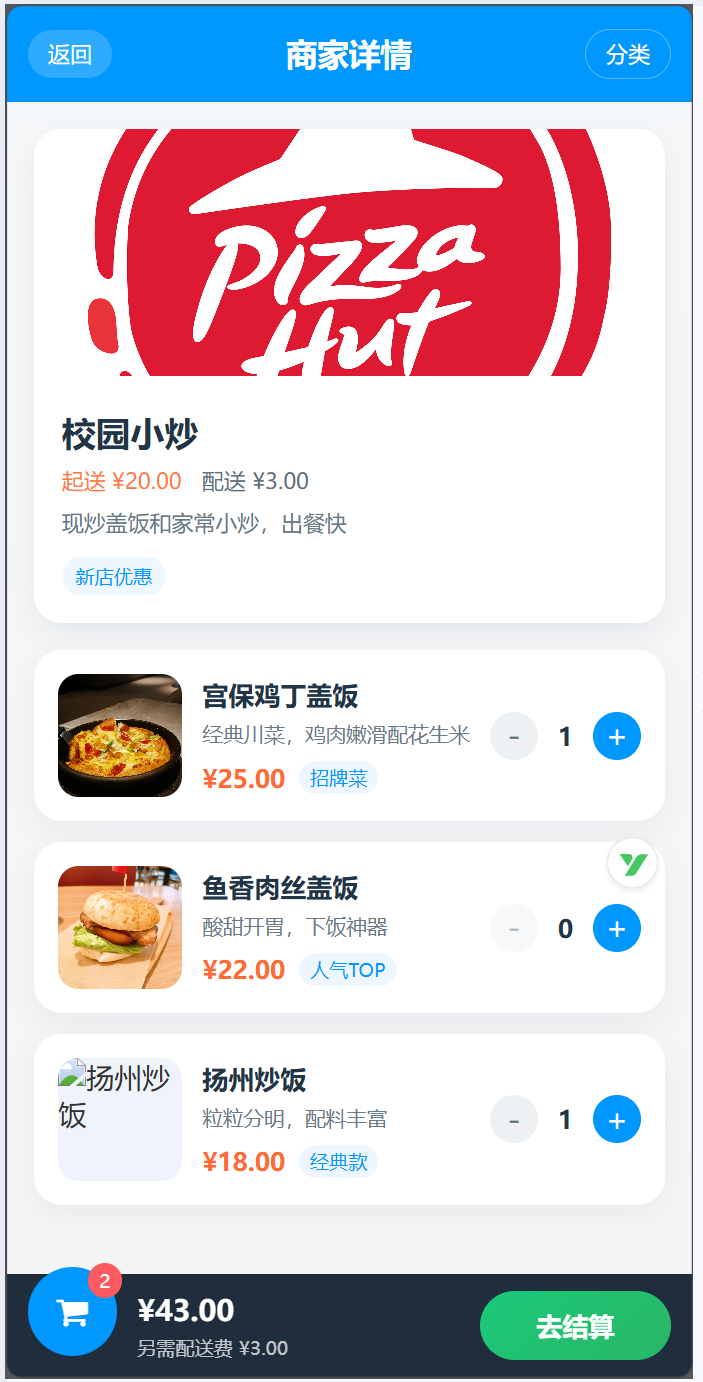
\includegraphics[width=0.75\textwidth,height=0.82\textheight,keepaspectratio]{images/page-business-info.png}
	\caption{商家详情页面}
	\label{fig:business-info-page}
\end{figure}

商家详情页面（BusinessInfo.vue）展示单个商家的完整信息，包括商家头图、名称、地址、简介、营业时间和备注。页面下方以列表形式展示该商家所有在售食品，每项食品显示名称、图片、价格（元）和简介，支持"加入购物车"按钮。食品列表通过\verb|GET /foods?businessId={id}|获取。

\subsection{商家管理页面}

\begin{figure}[H]
	\centering
	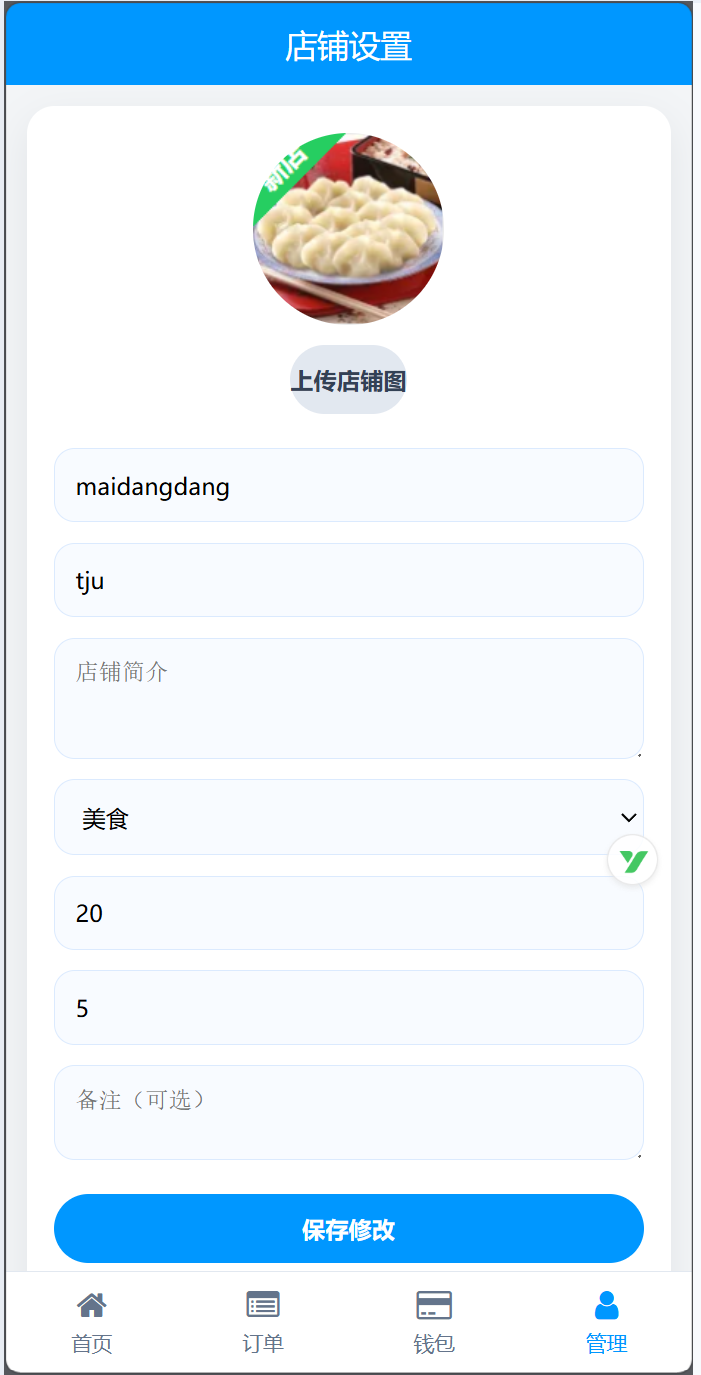
\includegraphics[width=0.75\textwidth,height=0.82\textheight,keepaspectratio]{images/page-business-manage.png}
	\caption{商家管理页面}
	\label{fig:business-manage-page}
\end{figure}

商家管理页面（BusinessManage.vue）展示当前用户拥有的商家列表，支持编辑商家信息。商家所有者可以查看该商家收到的订单列表。

\subsection{商家订单页面}

\begin{figure}[H]
	\centering
	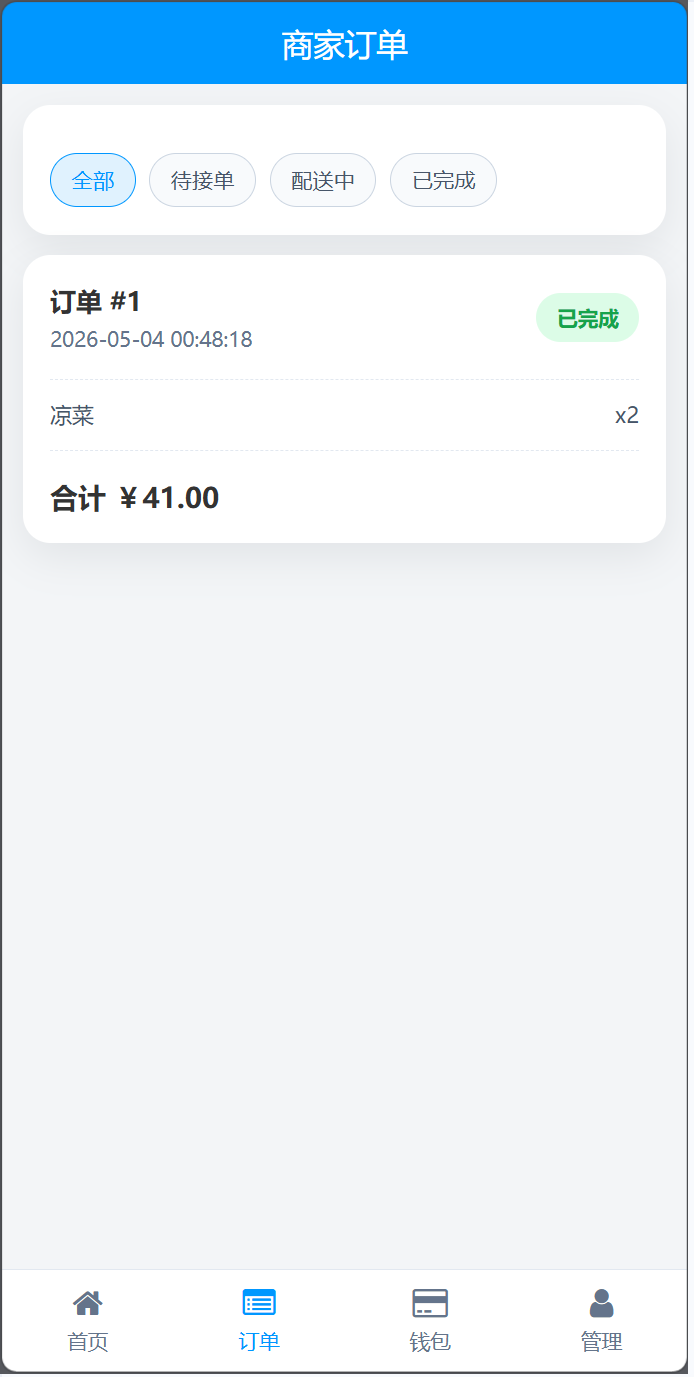
\includegraphics[width=0.75\textwidth,height=0.82\textheight,keepaspectratio]{images/page-business-orders.png}
	\caption{商家订单页面}
	\label{fig:business-orders-page}
\end{figure}

商家订单页面（BusinessOrders.vue）展示某商家收到的所有订单，支持按订单状态筛选（待支付/配送中/已送达/已完成），商家可以对订单执行确认支付、开始配送、完成配送等状态流转操作。

\section{食品与购物车模块}

\subsection{购物车页面}

\begin{figure}[H]
	\centering
	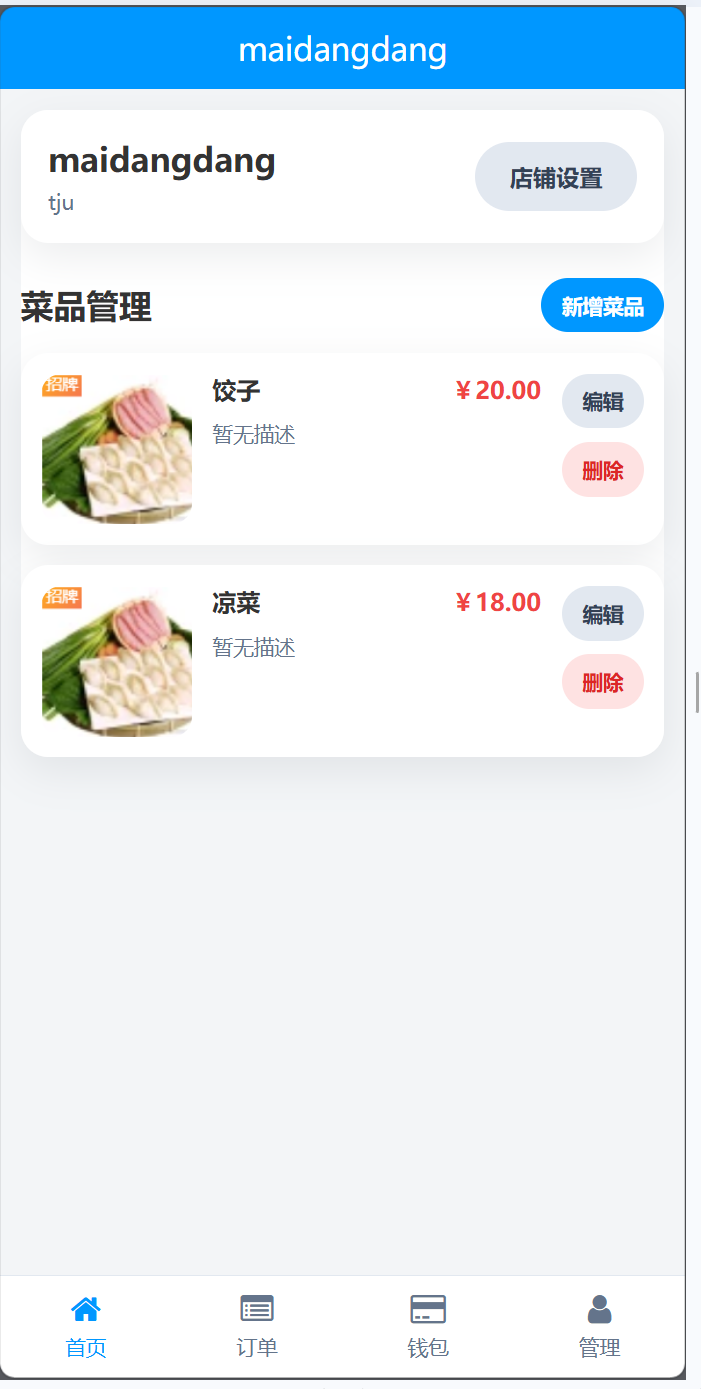
\includegraphics[width=0.75\textwidth,height=0.82\textheight,keepaspectratio]{images/page-cart.png}
	\caption{购物车页面}
	\label{fig:cart-page}
\end{figure}

购物车页面展示用户已添加的购物车项，按商家分组显示。每项显示食品名称、单价、数量和金额小计，支持修改数量和删除操作。底部合计显示总金额，提供"去结算"按钮进入下单流程。

\section{订单模块}

\subsection{订单结算页面}

\begin{figure}[H]
	\centering
	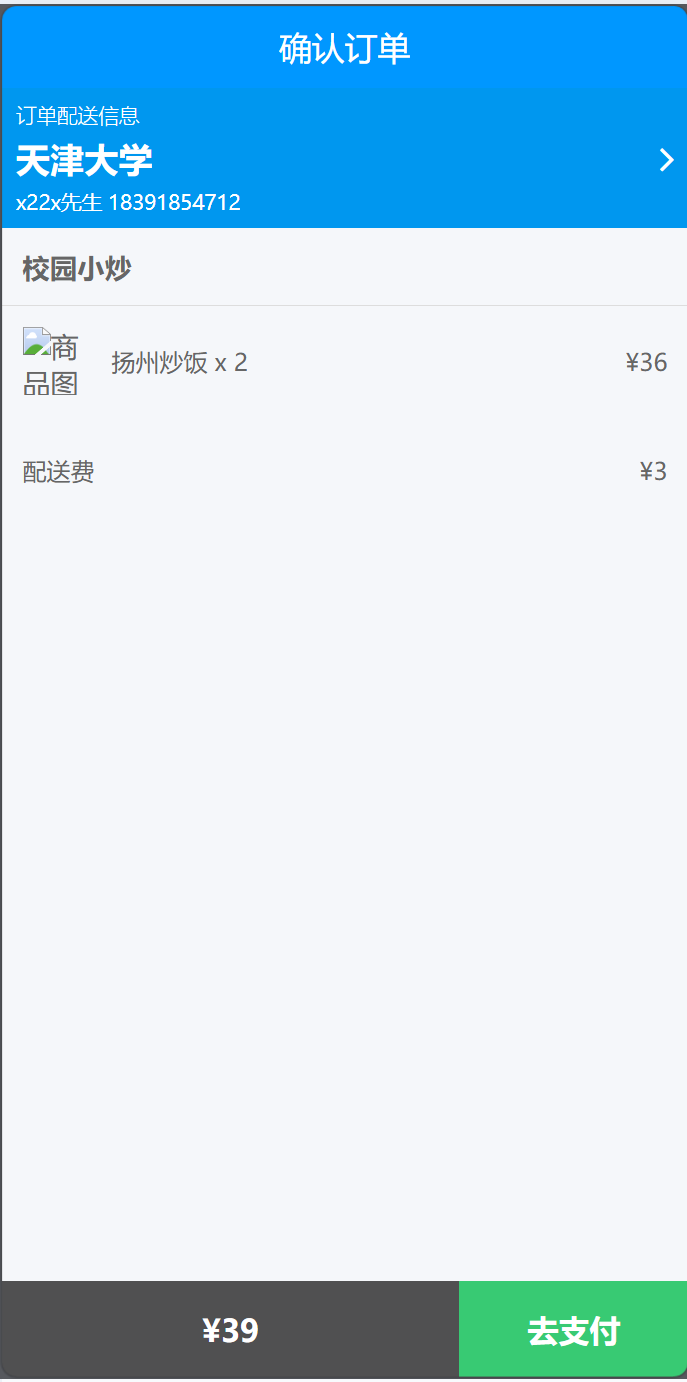
\includegraphics[width=0.75\textwidth,height=0.82\textheight,keepaspectratio]{images/page-order-checkout.png}
	\caption{订单结算页面}
	\label{fig:order-checkout-page}
\end{figure}

订单结算页面（Orders.vue）展示待提交订单的完整信息：配送地址选择、购物车商品明细、订单总金额、配送费明细。用户选择配送地址后确认下单，调用\verb|POST /orders|创建订单。

\subsection{用户订单列表页面}

\begin{figure}[H]
	\centering
	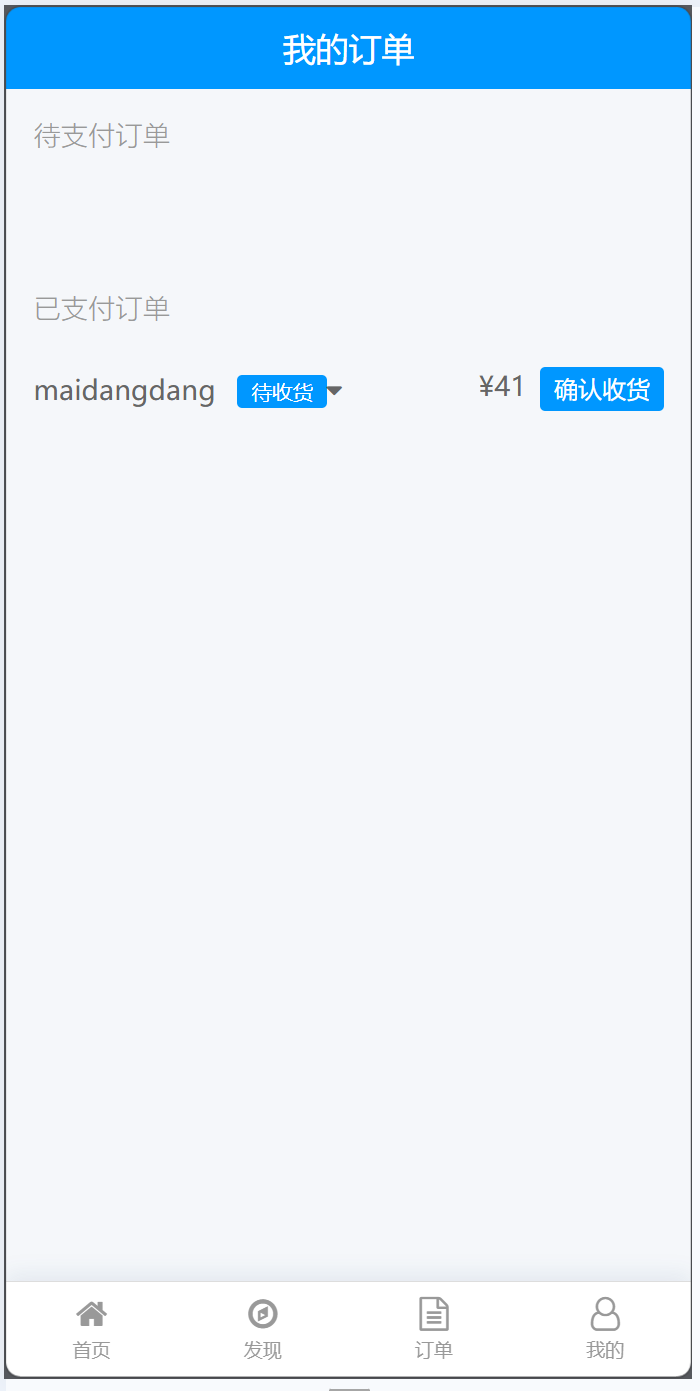
\includegraphics[width=0.75\textwidth,height=0.82\textheight,keepaspectratio]{images/page-user-order-list.png}
	\caption{用户订单列表页面}
	\label{fig:user-order-list-page}
\end{figure}

用户订单列表页面（OrderList.vue / UserOrderList.vue）展示当前用户的所有历史订单，按时间倒序排列。每个订单显示订单号、商家名称、订单总金额、订单状态（待支付/已支付/配送中/已送达/已完成）和下单时间。支持按订单状态筛选和查看订单详情。

\subsection{支付页面}

\begin{figure}[H]
	\centering
	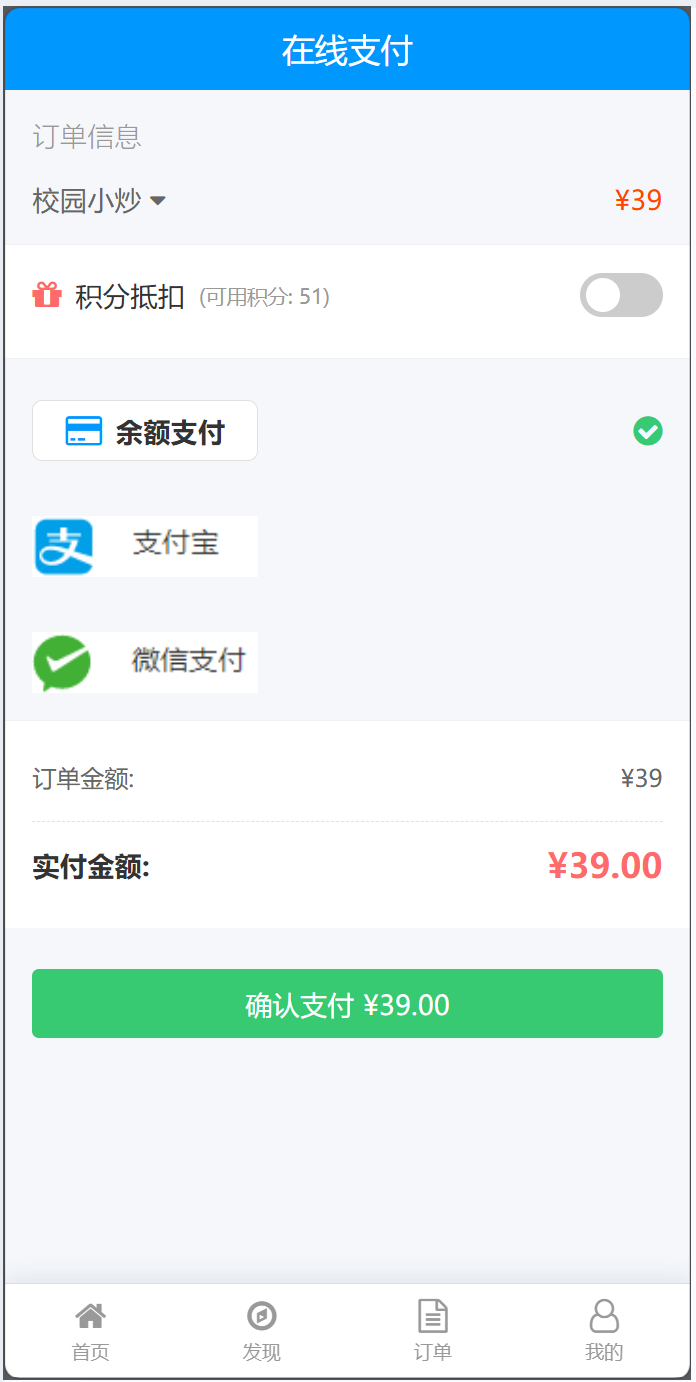
\includegraphics[width=0.75\textwidth,height=0.82\textheight,keepaspectratio]{images/page-payment.png}
	\caption{支付页面}
	\label{fig:payment-page}
\end{figure}

支付页面（Payment.vue）展示待支付订单的金额明细，支持虚拟钱包支付方式。用户确认支付后调用\verb|POST /orders/{id}/pay/virtual-wallet|，系统通过分布式锁保障交易一致性，扣除钱包余额并应用积分抵扣，更新订单状态为已支付。

\section{配送地址模块}

\subsection{地址管理页面}

\begin{figure}[H]
	\centering
	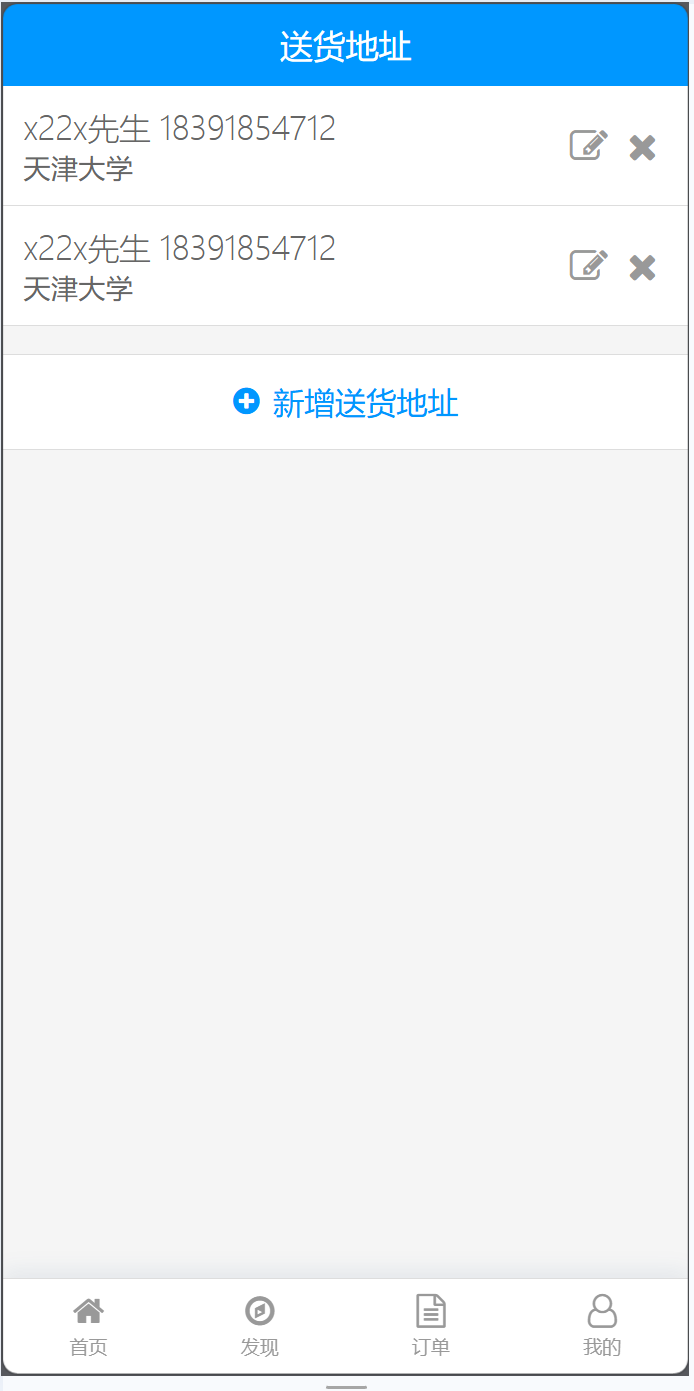
\includegraphics[width=0.75\textwidth,height=0.82\textheight,keepaspectratio]{images/page-user-address.png}
	\caption{地址管理页面}
	\label{fig:user-address-page}
\end{figure}

地址管理页面（UserAddress.vue）以列表形式展示用户所有有效配送地址，每项显示联系人姓名、性别、电话和详细地址。支持设为默认地址、编辑和删除操作。

\subsection{新增地址页面}

\begin{figure}[H]
	\centering
	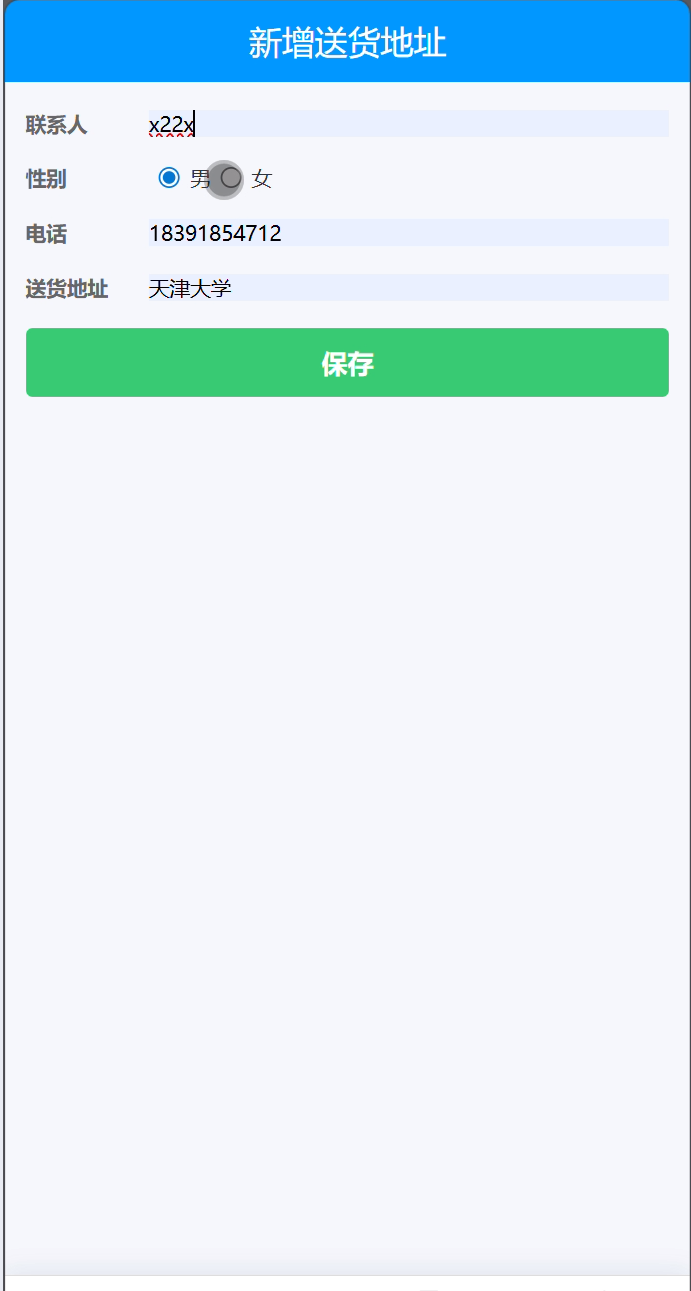
\includegraphics[width=0.75\textwidth,height=0.82\textheight,keepaspectratio]{images/page-add-address.png}
	\caption{新增地址页面}
	\label{fig:add-address-page}
\end{figure}

新增地址页面（AddUserAddress.vue）提供配送地址表单，包含联系人姓名、性别（单选）、联系电话、详细地址等字段。提交至\verb|POST /delivery-addresses|。

\subsection{编辑地址页面}

\begin{figure}[H]
	\centering
	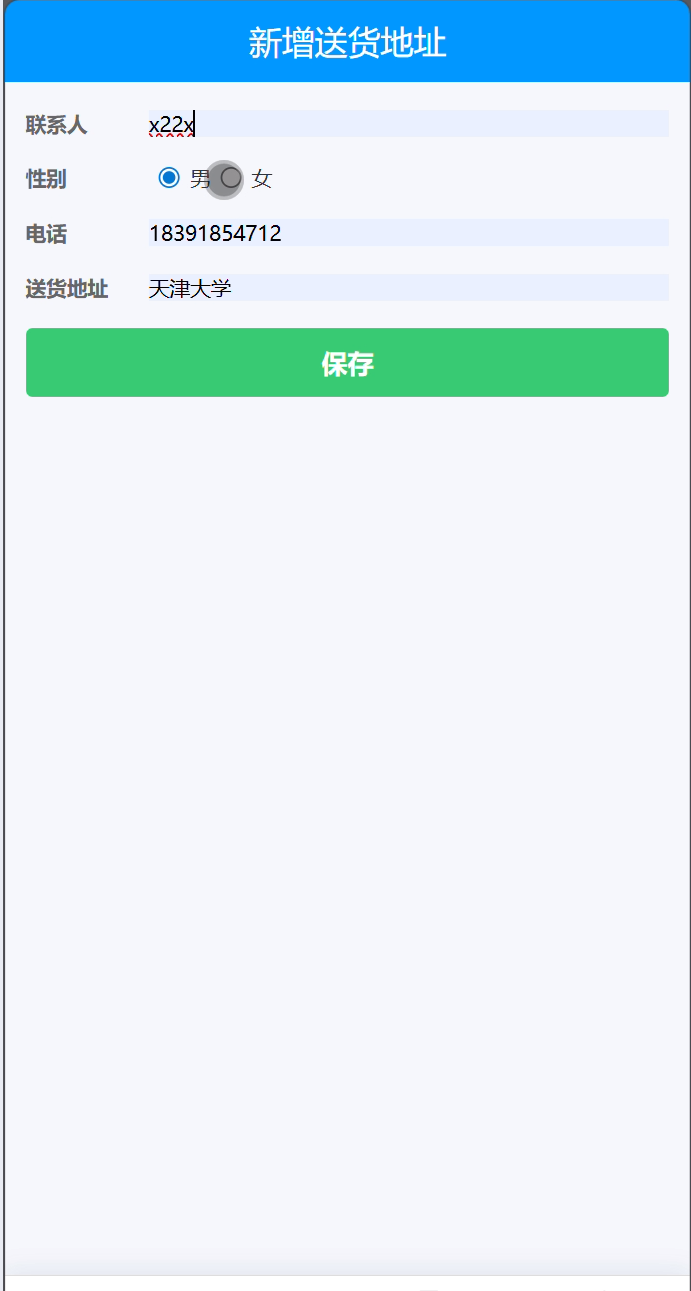
\includegraphics[width=0.75\textwidth,height=0.82\textheight,keepaspectratio]{images/page-edit-address.png}
	\caption{编辑地址页面}
	\label{fig:edit-address-page}
\end{figure}

编辑地址页面（EditUserAddress.vue）复用新增地址的表单结构，预填已有地址信息，修改后提交至\verb|PUT /delivery-addresses/{id}|。

\section{钱包模块}

\subsection{钱包页面}

\begin{figure}[H]
	\centering
	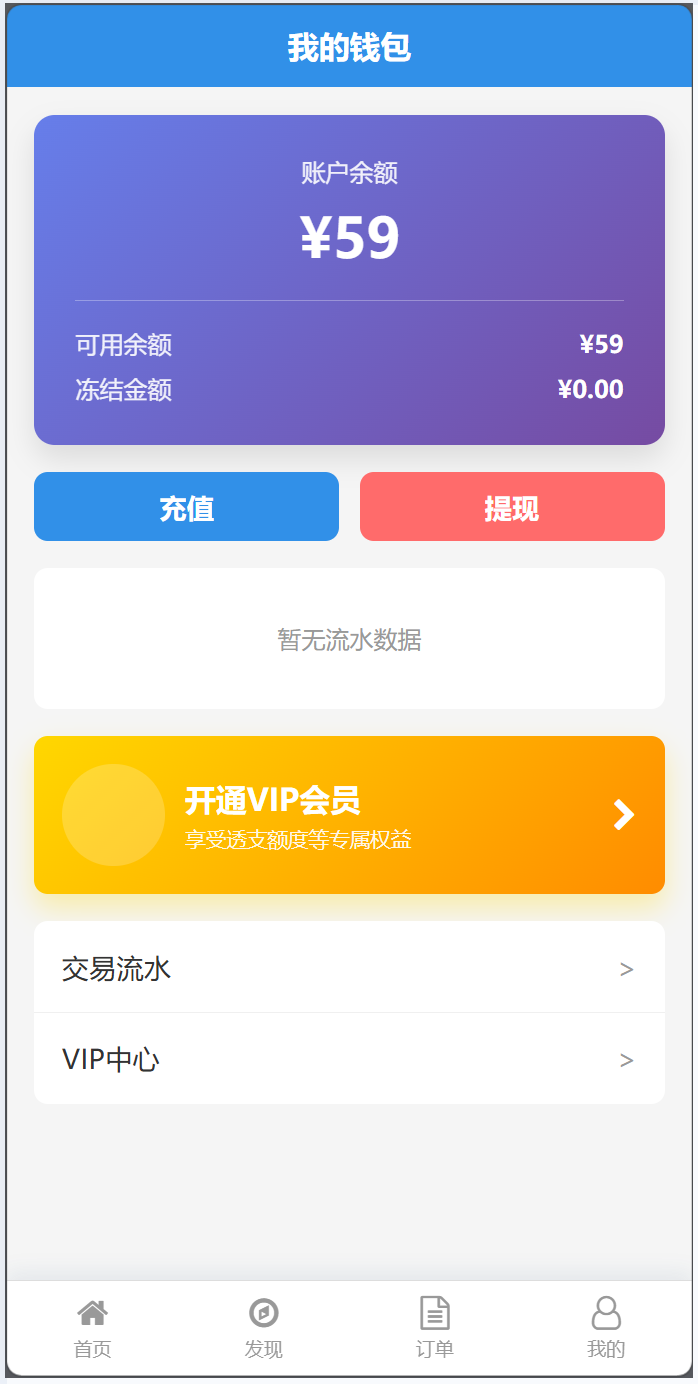
\includegraphics[width=0.75\textwidth,height=0.82\textheight,keepaspectratio]{images/page-wallet.png}
	\caption{钱包页面}
	\label{fig:wallet-page}
\end{figure}

钱包页面（Wallet.vue）展示用户虚拟钱包概览：当前余额（元）、信用额度、已用信用额度。下方提供充值、转账、提现、还款等操作入口。钱包交易的核心操作（充值、支付、转账）均受Redisson分布式锁保护。

\subsection{钱包充值页面}

\begin{figure}[H]
	\centering
	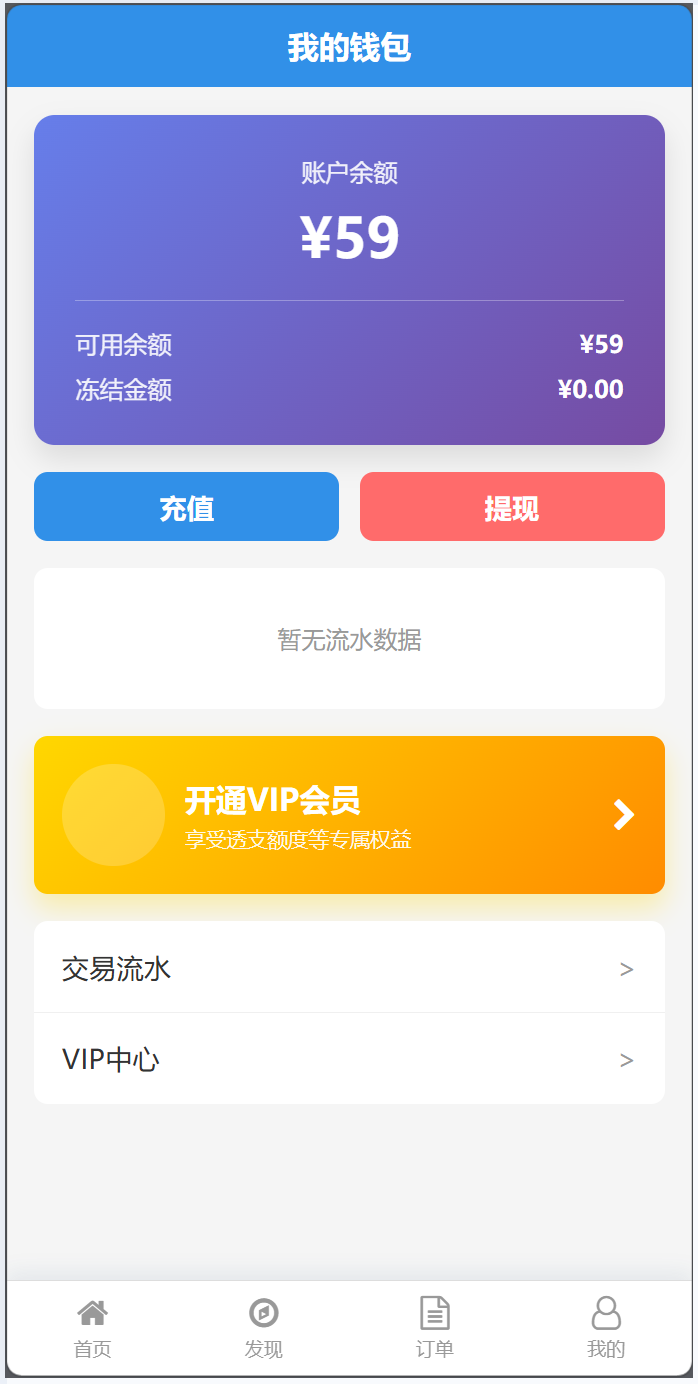
\includegraphics[width=0.75\textwidth,height=0.82\textheight,keepaspectratio]{images/page-wallet-recharge.png}
	\caption{钱包充值页面}
	\label{fig:wallet-recharge-page}
\end{figure}

钱包充值页面（WalletRecharge.vue）提供充值金额输入和支付方式选择，提交至\verb|POST /wallet/recharge|增加钱包余额。

\subsection{钱包提现页面}

\begin{figure}[H]
	\centering
	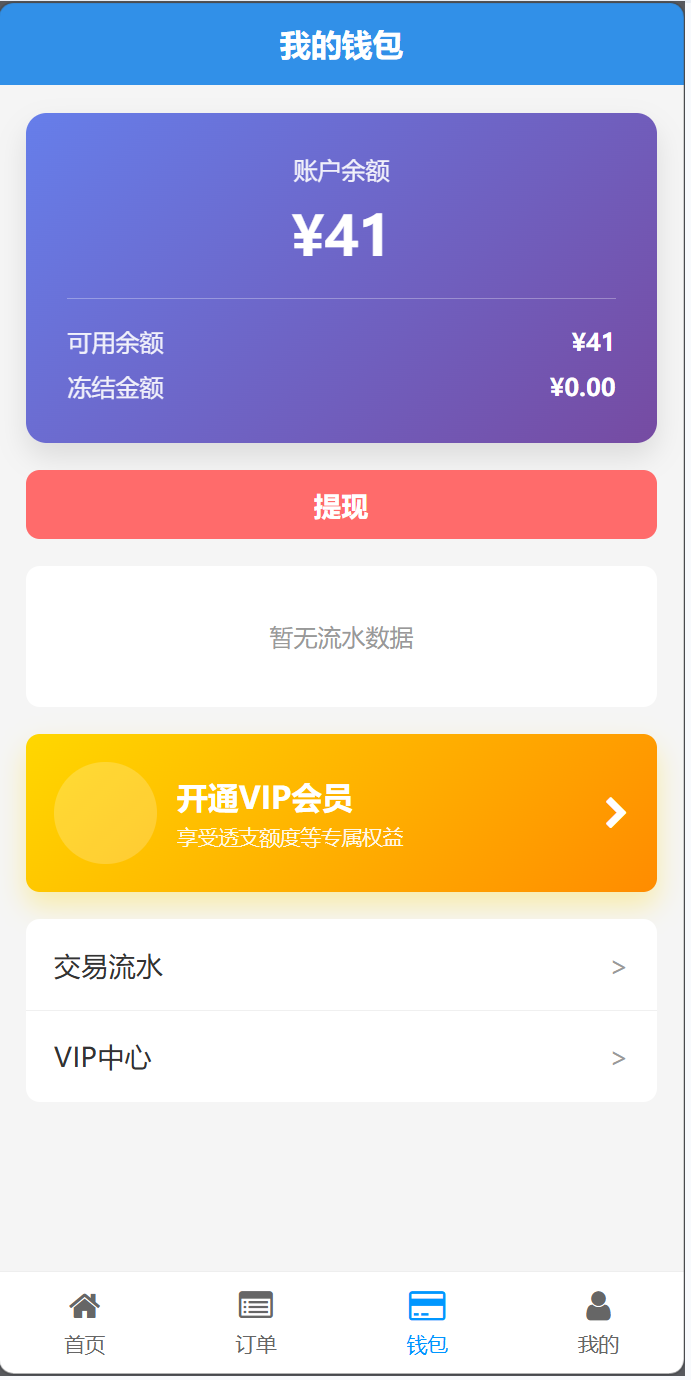
\includegraphics[width=0.75\textwidth,height=0.82\textheight,keepaspectratio]{images/page-wallet-withdraw.png}
	\caption{钱包提现页面}
	\label{fig:wallet-withdraw-page}
\end{figure}

钱包提现页面（WalletWithdraw.vue）允许用户将钱包余额提现至绑定的银行账户或支付平台。


\section{积分模块}

\subsection{积分概览页面}

\begin{figure}[H]
	\centering
	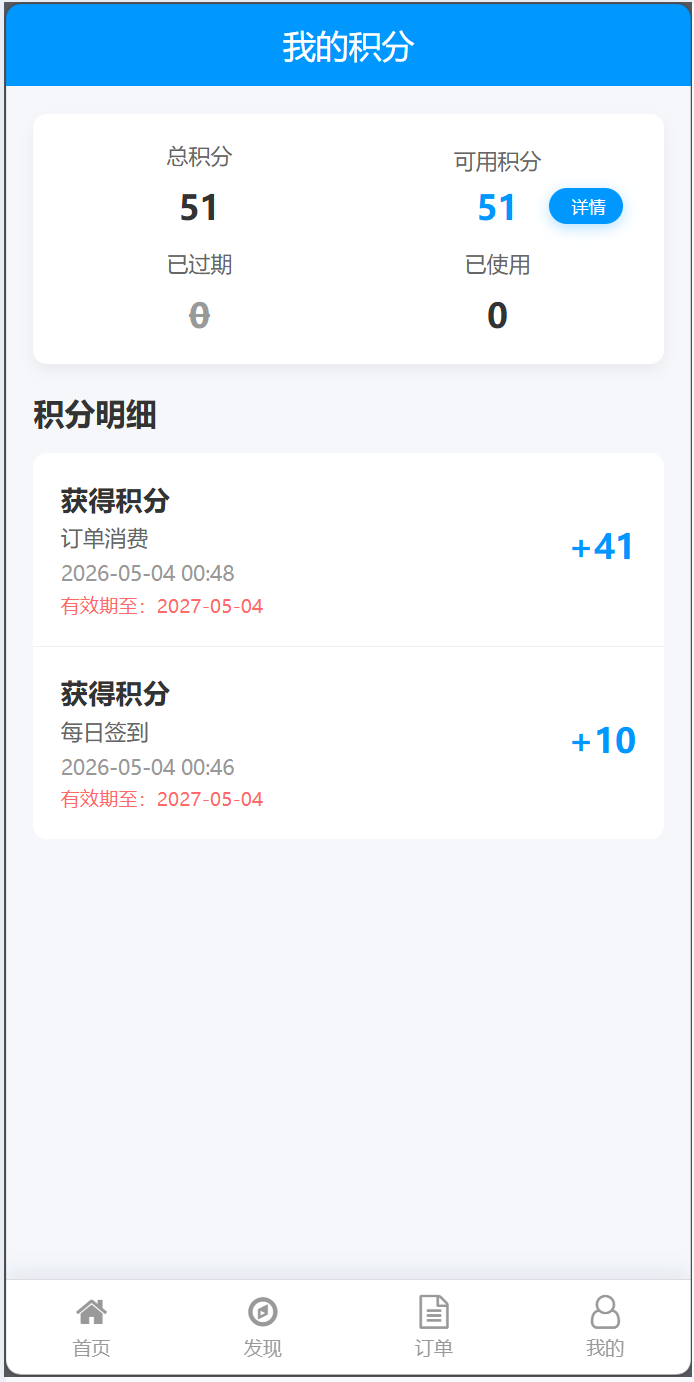
\includegraphics[width=0.75\textwidth,height=0.82\textheight,keepaspectratio]{images/page-points.png}
	\caption{积分概览页面}
	\label{fig:points-page}
\end{figure}

积分概览页面（Points.vue）展示用户积分统计信息：总积分、可用积分、已用积分、即将过期积分。下方提供签到、积分商城、积分明细等快捷入口。

\subsection{每日签到页面}

\begin{figure}[H]
	\centering
	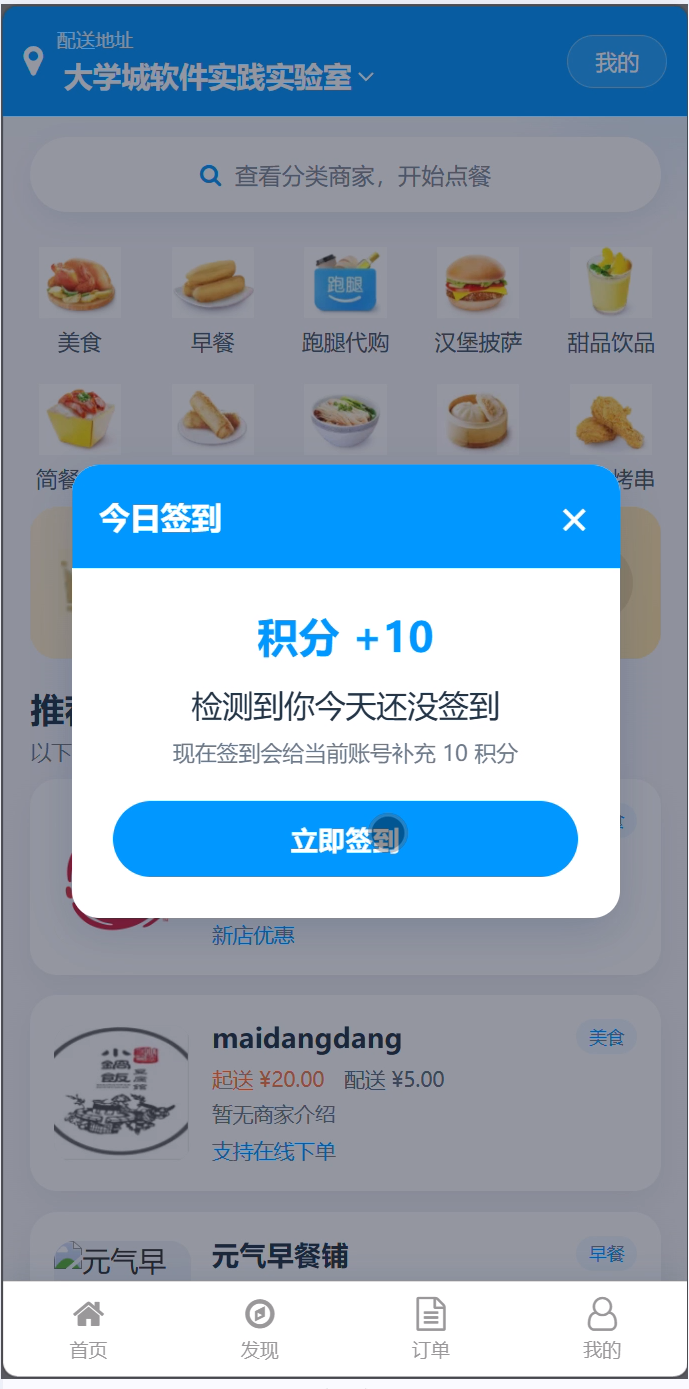
\includegraphics[width=0.75\textwidth,height=0.82\textheight,keepaspectratio]{images/page-signin.png}
	\caption{每日签到页面}
	\label{fig:signin-page}
\end{figure}

签到功能嵌入积分页面，用户每日点击签到按钮调用\verb|POST /integral/signIn|。前端展示连续签到天数和当日获得的积分奖励。连续签到天数越多，单日奖励越高，激励用户保持活跃。

\subsection{积分商城页面}

\begin{figure}[H]
	\centering
	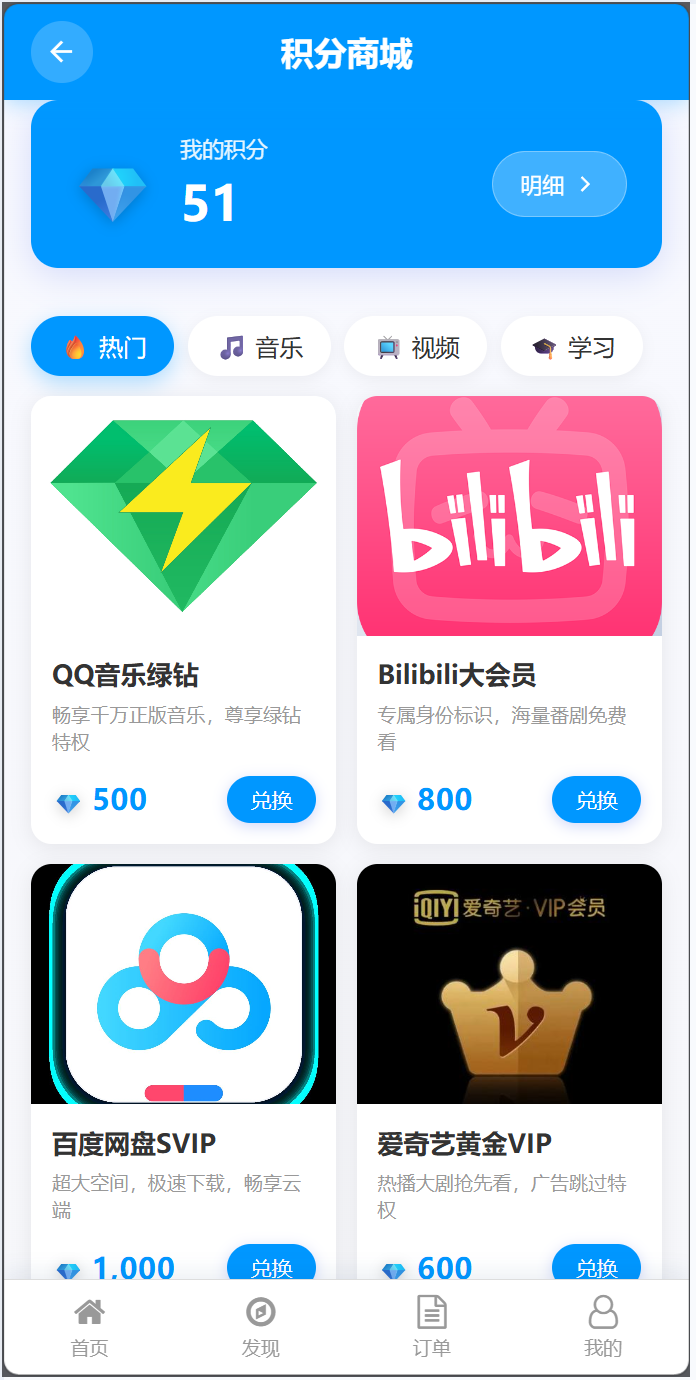
\includegraphics[width=0.75\textwidth,height=0.82\textheight,keepaspectratio]{images/page-points-mall.png}
	\caption{积分商城页面}
	\label{fig:points-mall-page}
\end{figure}

积分商城页面（PointsMall.vue）展示可使用积分兑换的商品列表（如优惠券、代金券等），每项商品显示所需积分和库存数量。用户点击兑换调用\verb|POST /integral/exchange|，扣除积分并生成兑换记录。


\section{管理员模块}

\subsection{管理员登录页面}

\begin{figure}[H]
	\centering
	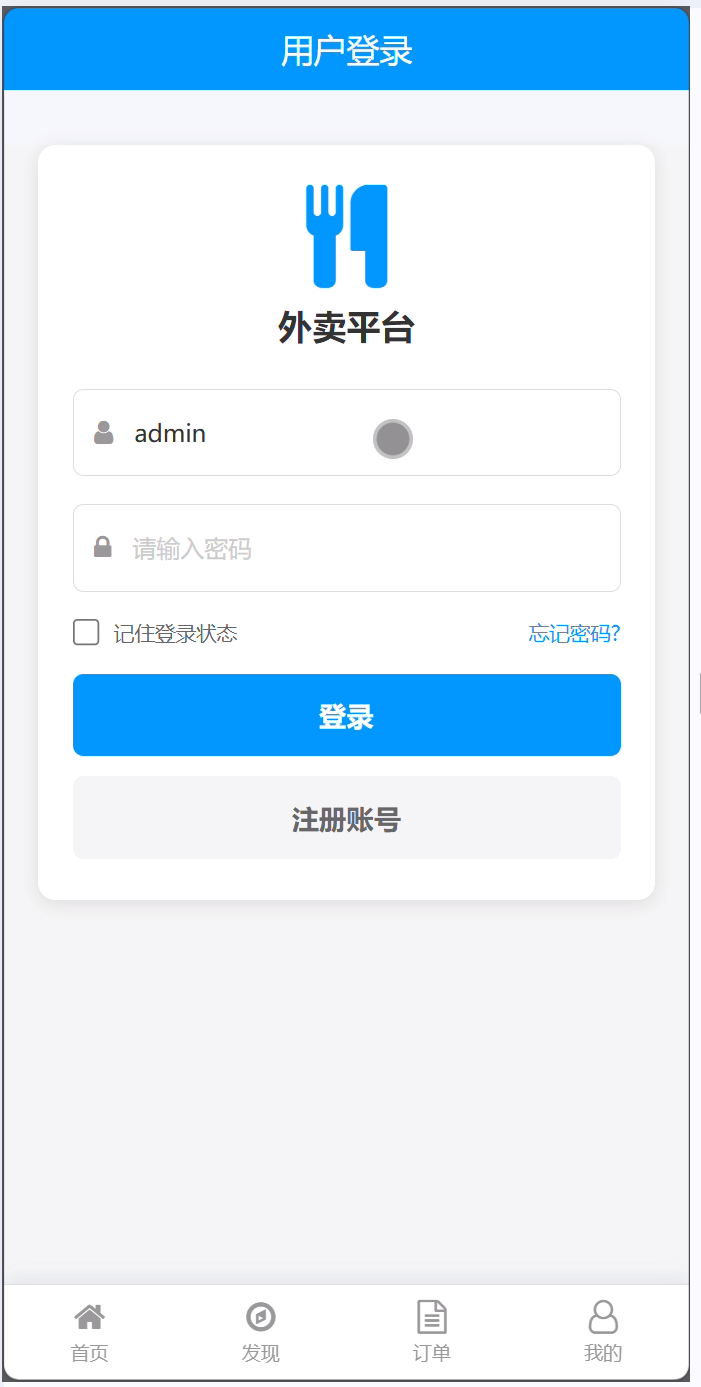
\includegraphics[width=0.75\textwidth,height=0.82\textheight,keepaspectratio]{images/page-admin-login.png}
	\caption{管理员登录页面}
	\label{fig:admin-login-page}
\end{figure}

管理员登录页面（AdminLogin.vue）提供管理员专属登录入口，与普通用户登录隔离，使用独立的管理员认证逻辑。

\subsection{用户管理页面}

\begin{figure}[H]
	\centering
	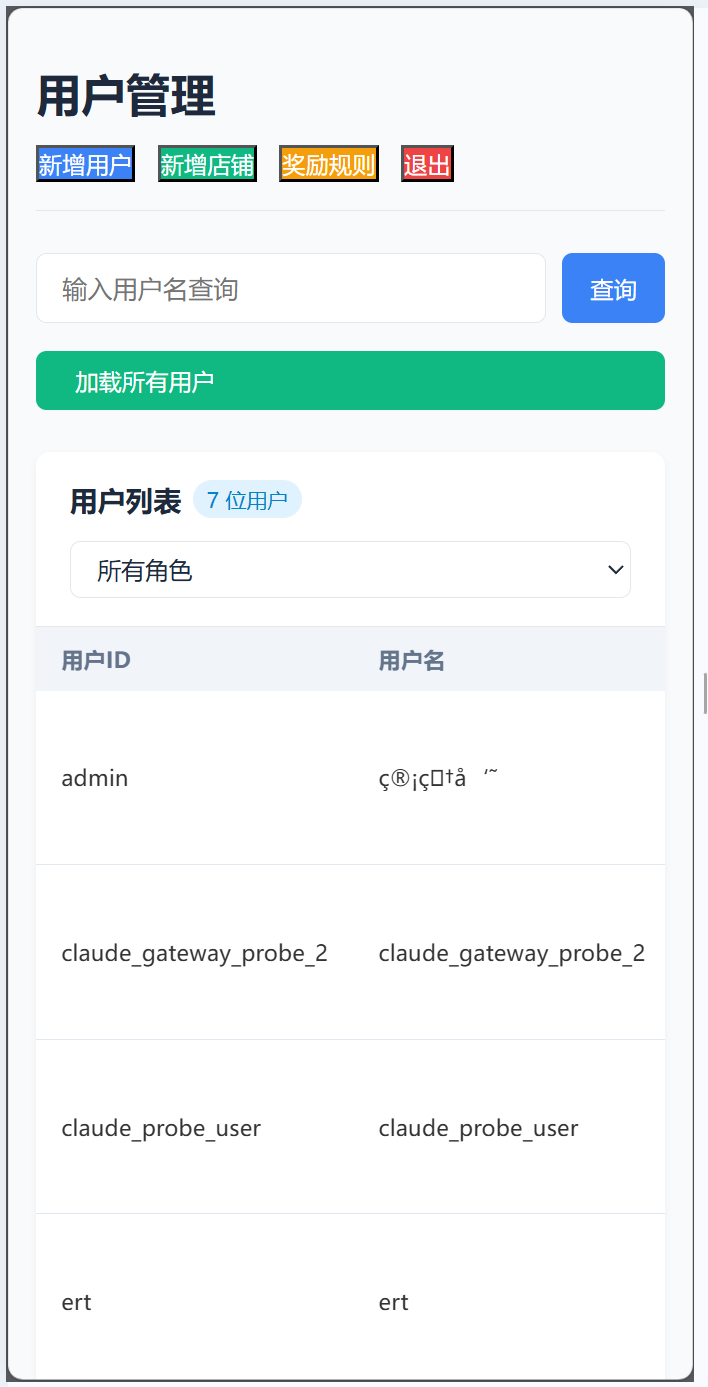
\includegraphics[width=0.75\textwidth,height=0.82\textheight,keepaspectratio]{images/page-user-management.png}
	\caption{用户管理页面}
	\label{fig:user-management-page}
\end{figure}

用户管理页面（UserManagement.vue）以表格形式展示系统所有注册用户，支持按用户名搜索、查看用户详情、启用/禁用用户账号等操作。

\subsection{添加用户页面}

\begin{figure}[H]
	\centering
	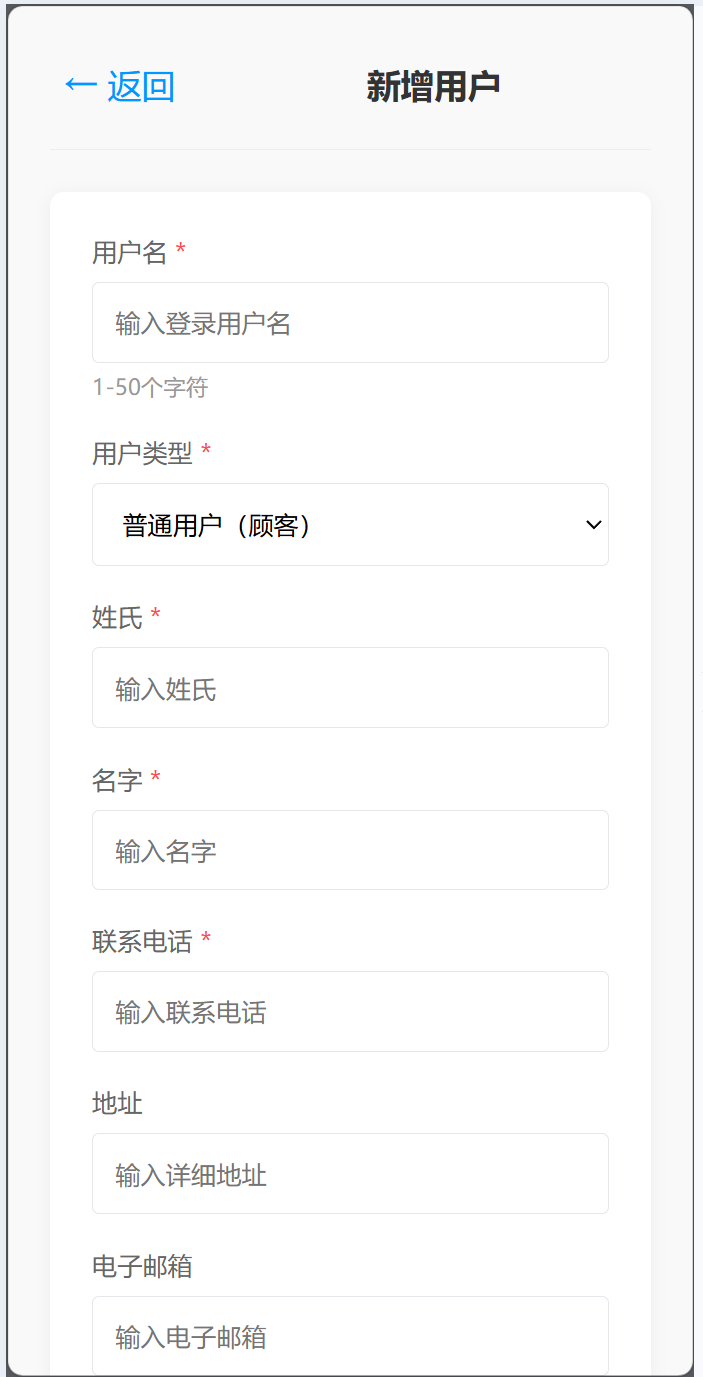
\includegraphics[width=0.75\textwidth,height=0.82\textheight,keepaspectratio]{images/page-add-user.png}
	\caption{添加用户页面}
	\label{fig:add-user-page}
\end{figure}

添加用户页面（AddUser.vue）允许管理员直接创建新用户账号，设置初始密码和基本信息。

\section{用户信息模块}

\subsection{用户信息页面}

\begin{figure}[H]
	\centering
	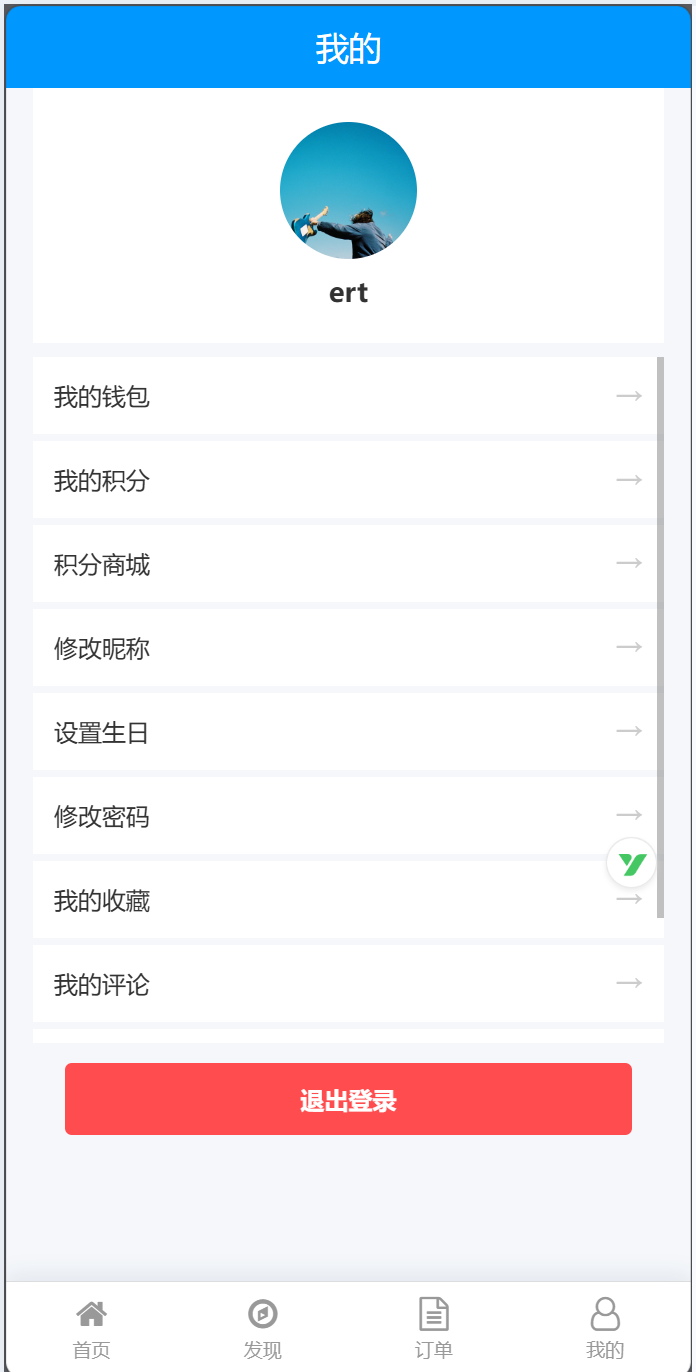
\includegraphics[width=0.75\textwidth,height=0.82\textheight,keepaspectratio]{images/page-user-info.png}
	\caption{用户信息页面}
	\label{fig:user-info-page}
\end{figure}

用户信息页面（UserInfo.vue）展示和编辑当前用户的个人资料，包括用户名、头像、性别、注册时间等。支持修改头像（上传图片）和更新基本信息。

\section{前端技术实现要点}

前端项目在技术实现上具有以下特点：

\begin{itemize}
	\item \textbf{路由管理}：使用Vue Router实现SPA路由，配置路由守卫（beforeEach）检查登录状态，未登录用户访问需认证页面时自动跳转至登录页
	\item \textbf{HTTP通信}：使用Axios封装统一的HTTP客户端，配置请求拦截器自动附加JWT Token，配置响应拦截器统一处理错误（如401未授权跳转登录页）
	\item \textbf{状态管理}：使用Vuex管理全局状态（用户信息、购物车数量徽标等）
	\item \textbf{UI组件}：使用Element Plus组件库（el-table、el-form、el-dialog、el-card等）构建统一风格的用户界面
	\item \textbf{数据可视化}：使用ECharts实现积分趋势图表、消费统计饼图等数据可视化展示
	\item \textbf{响应式布局}：使用Flex布局和Element Plus的Layout组件实现PC端和移动端的适配
	\item \textbf{容错提示}：集成GlobalFallbackRetryPrompt组件，在检测到后端服务降级响应时向用户展示友好的提示信息和重试选项
\end{itemize}

   % 前端页面展示
	% !Mode:: "TeX:UTF-8"

\chapter{测试设计与结果}

本项目为8个微服务模块编写了19个测试类，覆盖Controller层、Service层、Mapper层及边界条件测试。测试框架基于JUnit 5 + Mockito + Spring Boot Test，遵循分层测试策略。

\section{测试框架与工具}

\begin{table}[H]
	\centering
	\caption{测试技术栈一览}
	\begin{tabular}{p{5.0cm}p{5.0cm}p{4.0cm}}
		\hline
		\textbf{层面} & \textbf{技术} & \textbf{版本} \\
		\hline
		测试框架 & JUnit 5 (Jupiter) & 5.7.x \\
		Mock框架 & Mockito & 3.9.x \\
		Web层测试 & Spring MockMvc & -- \\
		集成测试 & Spring Boot Test & 2.4.5 \\
		断言库 & JUnit Assertions + Mockito Verify & -- \\
		JSON序列化 & Jackson ObjectMapper & -- \\
		\hline
	\end{tabular}
\end{table}

\section{测试架构设计}

本项目采用四层测试金字塔架构，自底向上覆盖Mapper层、Service层、Controller层和边界场景：

\begin{enumerate}
	\item \textbf{Mapper层测试}（1个测试类）：使用\verb|@SpringBootTest| + \verb|@Transactional|，测试真实数据库的CRUD操作，验证事务自动回滚，确保不污染数据库
	\item \textbf{Service层单元测试}（4个测试类）：使用\verb|@ExtendWith(MockitoExtension.class)|，Mock Mapper和Feign客户端，验证业务逻辑的正确性
	\item \textbf{Controller层测试}（11个测试类）：使用\verb|MockMvcBuilders.standaloneSetup|独立模式，Mock Service层，验证HTTP请求/响应、状态码和JSON结构
	\item \textbf{边界条件测试}（3个测试类）：针对空列表、null值、零数量、重复操作、订单不存在等边界场景，确保系统鲁棒性
\end{enumerate}

\section{测试模块总览}

\begin{table}[H]
	\centering
	\caption{各模块测试统计}
	\begin{tabular}{p{5.5cm}p{1.8cm}p{2.8cm}p{4.0cm}}
		\hline
		\textbf{模块} & \textbf{测试类数} & \textbf{用例数} & \textbf{测试层级} \\
		\hline
		elm-user-server & 1 & 20 & Controller (MockMvc) \\
		elm-business-server & 4 & 28 & Controller + Service + Boundary \\
		elm-food-server & 1 & 2 & Controller (MockMvc) \\
		elm-cart-server & 3 & 15 & Controller + Service + Boundary \\
		elm-order-server & 2 & 15 & Controller + Service (SpringBootTest) \\
		elm-delivery-server & 2 & 7 & Controller + Service (SpringBootTest) \\
		elm-wallet-server & 2 & 6 & Controller + Service \\
		elm-point-server & 4 & 38 & Controller + Service + Mapper + Feign \\
		\hline
		\textbf{合计} & \textbf{19} & \textbf{131} & -- \\
		\hline
	\end{tabular}
\end{table}

\section{用户微服务测试 (elm-user-server)}

\subsection{测试设计}

UserControllerTest（20个用例）基于MockMvc独立模式，Mock UserService和JwtTokenProvider，覆盖以下场景：

\begin{itemize}
	\item \textbf{JWT认证}：验证有效Token返回用户信息（HTTP 200）、无效Token返回401
	\item \textbf{登录认证}：正确凭据返回JWT Token并设置Authorization Header、错误密码返回401
	\item \textbf{密码修改}：验证Token后修改密码成功返回200
	\item \textbf{用户信息更新}：更新本人信息成功（200）、更新他人信息被拒绝（403）
	\item \textbf{用户列表}：获取所有用户列表（200）
	\item \textbf{用户注册}：支持新旧两种注册路径（/api/register 和 /api/users），用户名冲突返回409
	\item \textbf{用户查询}：按用户名查询、按用户ID查询、检查用户存在性
	\item \textbf{边界场景}：缺少必填参数返回400、无Token请求受保护接口返回401
\end{itemize}

\subsection{测试结果}

\begin{figure}[H]
	\centering
	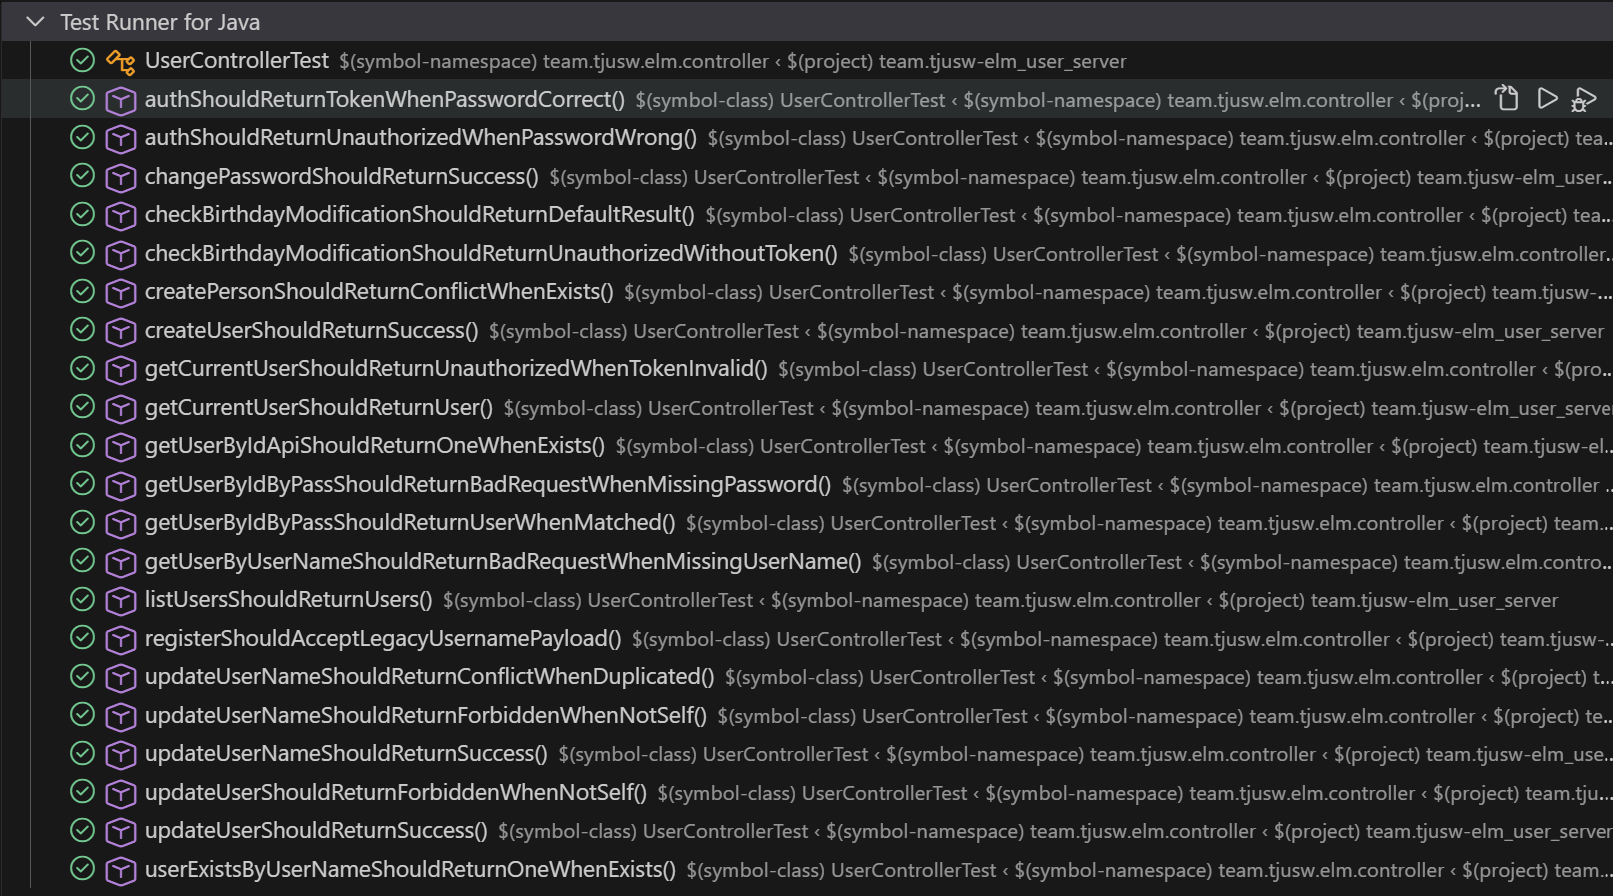
\includegraphics[width=0.85\textwidth,height=0.82\textheight,keepaspectratio]{images/test-user-controller-result.png}
	\caption{用户微服务测试结果}
	\label{fig:test-user-controller}
\end{figure}

\section{商家微服务测试 (elm-business-server)}

\subsection{测试设计}

商家模块包含4个测试类，覆盖Controller和Service两层：

\textbf{BusinessControllerTest}（2个用例）：测试商家创建（POST /businesses，期望返回201和完整商家对象）、商家信息更新（PUT /businesses/\{id\}，验证更新后字段值）。

\textbf{OrderControllerTest}（9个用例）：测试订单创建（POST /orders，期望201）、用户订单列表、商家订单列表、订单详情、订单明细、支付/配送/完成订单状态流转（各期望200）。

\textbf{OrderServiceImplTest}（9个用例）：Mock OrderMapper和RabbitMQSender，测试创建订单（验证saveOrder和saveOrderDetail调用次数）、各类订单查询、更新订单状态（验证RabbitMQ消息发送）、支付/配送/完成订单。

\textbf{OrderServiceImplBoundaryTest}（8个用例）：测试空订单详情创建（验证总金额为0.0）、各类操作在订单不存在时返回0（不发送MQ消息）、查询返回空列表、查询返回null。

\subsection{测试结果}

\begin{figure}[H]
	\centering
	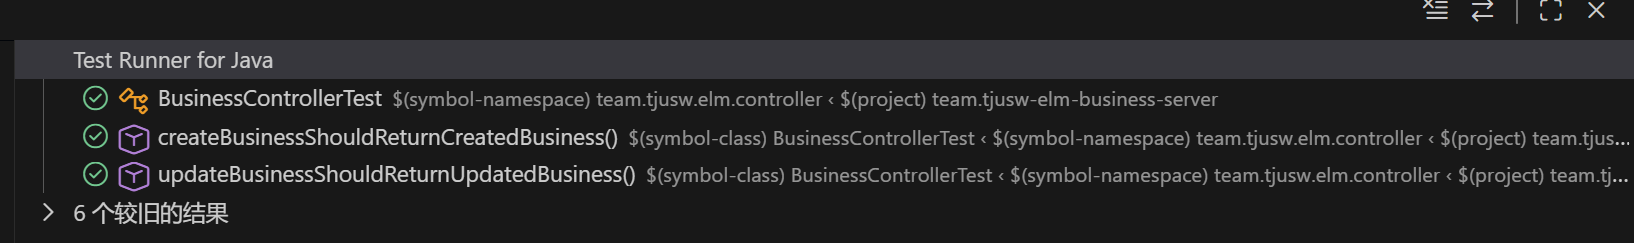
\includegraphics[width=0.85\textwidth,height=0.82\textheight,keepaspectratio]{images/test-business-controller-result.png}
	\caption{商家微服务BusinessController测试结果}
	\label{fig:test-business-controller}
\end{figure}

\begin{figure}[H]
	\centering
	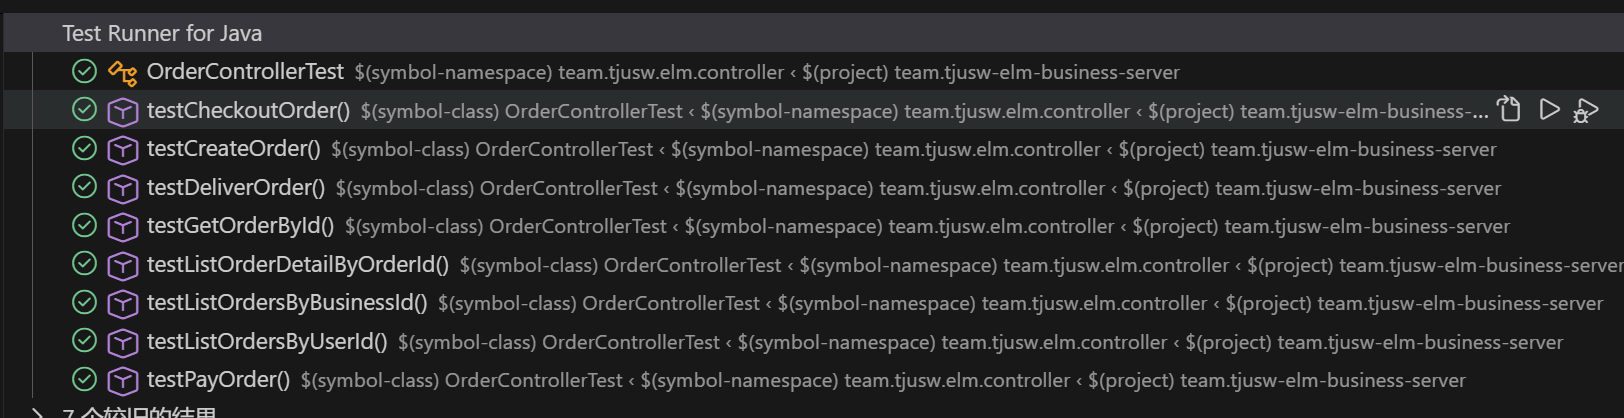
\includegraphics[width=0.85\textwidth,height=0.82\textheight,keepaspectratio]{images/test-order-controller-result.png}
	\caption{商家微服务OrderController测试结果}
	\label{fig:test-order-controller}
\end{figure}

\begin{figure}[H]
	\centering
	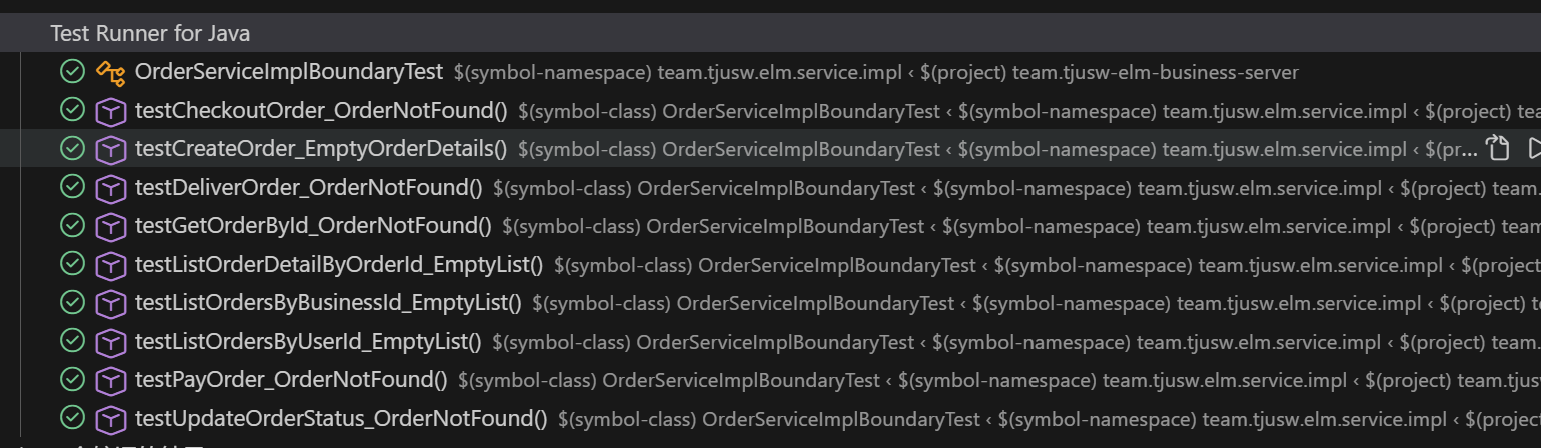
\includegraphics[width=0.85\textwidth,height=0.82\textheight,keepaspectratio]{images/test-order-service-result.png}
	\caption{OrderServiceImpl单元测试结果}
	\label{fig:test-order-service}
\end{figure}


\section{食品微服务测试 (elm-food-server)}

\subsection{测试设计}

FoodControllerTest（2个用例）基于MockMvc，测试食品新增和更新：

\begin{itemize}
	\item \textbf{新增食品}：POST /foods，提交食品对象（含BigDecimal价格），期望返回200且result为true
	\item \textbf{更新食品}：PUT /foods/\{id\}，验证返回对象中的foodId和foodName与预期一致
\end{itemize}

\subsection{测试结果}

\begin{figure}[H]
	\centering
	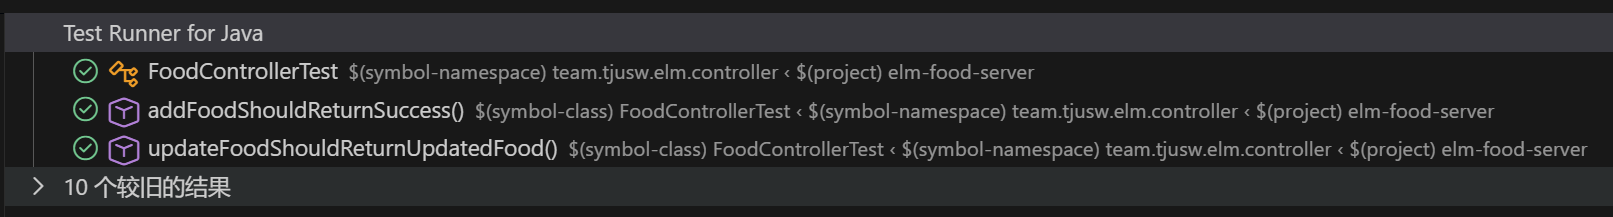
\includegraphics[width=0.85\textwidth,height=0.82\textheight,keepaspectratio]{images/test-food-controller-result.png}
	\caption{食品微服务测试结果}
	\label{fig:test-food-controller}
\end{figure}

\section{购物车微服务测试 (elm-cart-server)}

\subsection{测试设计}

购物车模块包含3个测试类：

\textbf{CartControllerTest}（5个用例）：MockMvc模式测试按用户ID获取购物车列表、按用户和商家获取、按用户和商家和食品删除、新增购物车项（期望201）、更新数量。

\textbf{CartServiceImplTest}（5个用例）：Mock CartMapper，测试新增购物车项——区分"新项插入"（验证insertCart调用、不调updateCart）和"已存在项更新"（验证updateCart调用、不调insertCart）；删除和查询验证返回值正确性和Mock调用次数。

\textbf{CartServiceImplBoundaryTest}（7个用例）：测试空购物车对象新增、零数量商品、删除不存在的项（返回0）、空列表查询、更新不存在的项（返回0）、零数量更新、已存在项零数量覆盖。

\subsection{测试结果}

\begin{figure}[H]
	\centering
	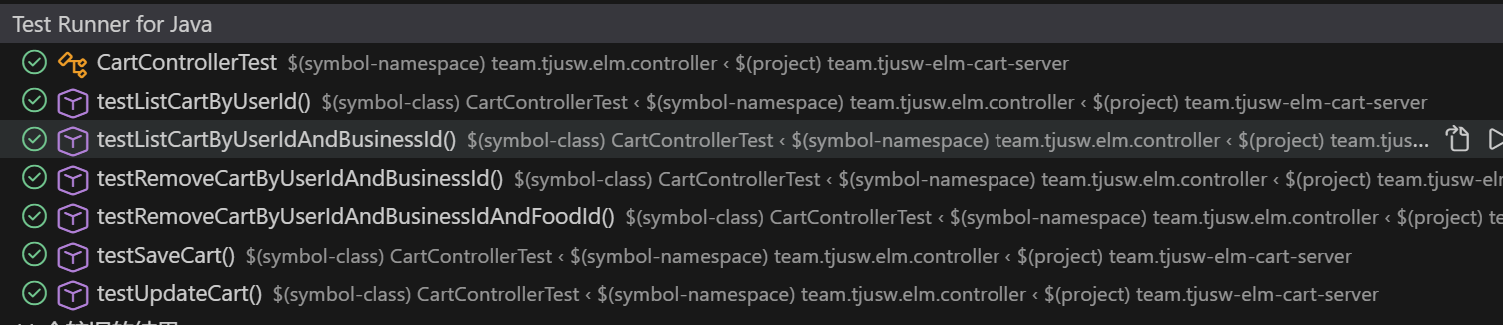
\includegraphics[width=0.85\textwidth,height=0.82\textheight,keepaspectratio]{images/test-cart-controller-result.png}
	\caption{购物车Controller测试结果}
	\label{fig:test-cart-controller}
\end{figure}

\begin{figure}[H]
	\centering
	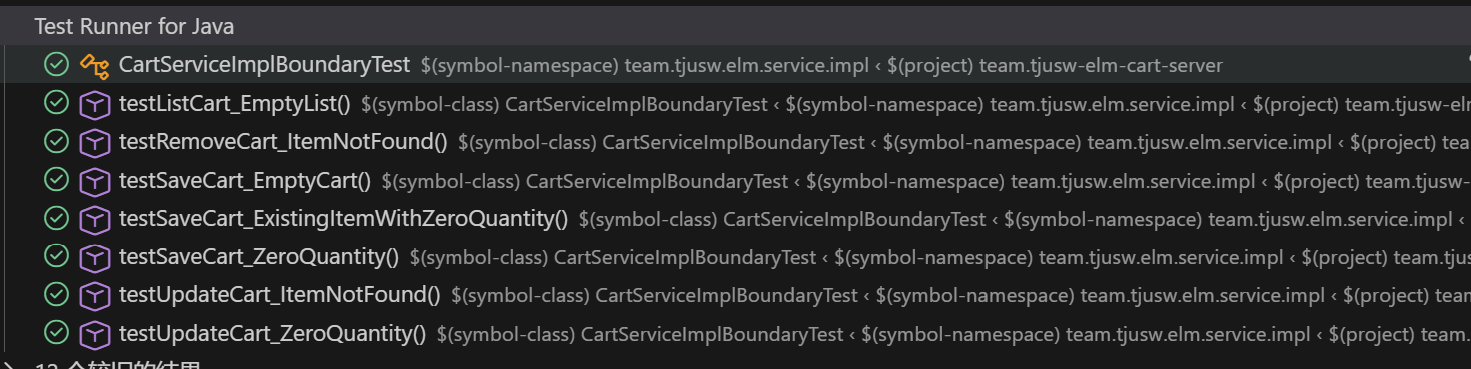
\includegraphics[width=0.85\textwidth,height=0.82\textheight,keepaspectratio]{images/test-cart-service-result.png}
	\caption{CartServiceImpl单元测试结果}
	\label{fig:test-cart-service}
\end{figure}

\begin{figure}[H]
	\centering
	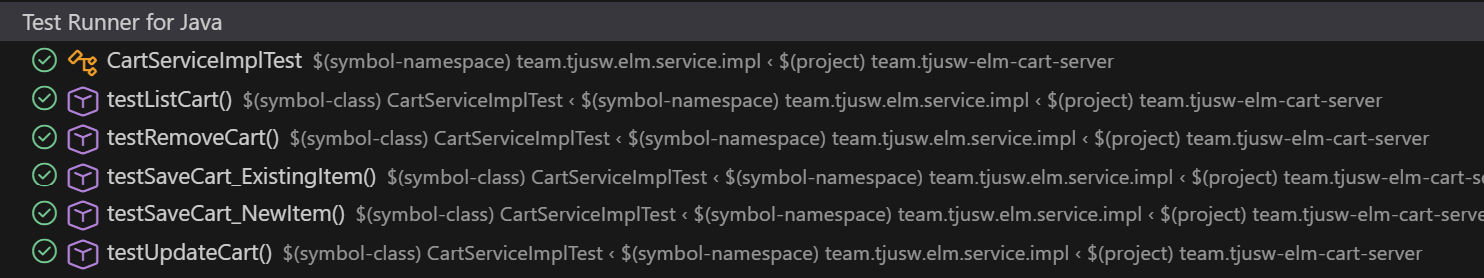
\includegraphics[width=0.85\textwidth,height=0.82\textheight,keepaspectratio]{images/test-cart-boundary-result.png}
	\caption{购物车边界条件测试结果}
	\label{fig:test-cart-boundary}
\end{figure}

\section{订单微服务测试 (elm-order-server)}

\subsection{测试设计}

订单模块包含2个SpringBootTest集成测试类，使用\verb|@MockBean|模拟所有Feign客户端（CartClient、VirtualWalletClient、PointClient、BusinessClient），\verb|@Transactional|自动回滚：

\textbf{OrdersServiceTest}（8个用例）：
\begin{itemize}
	\item 按用户ID和商家ID查询订单列表
	\item 按订单ID查询订单详情（含orderDetailet明细）
	\item 更新订单状态并验证持久化
	\item 创建订单——Mock购物车数据（LinkedHashMap模拟），验证orderDetailet写入正确数量
	\item 虚拟钱包支付成功——Mock完整Feign调用链（获取商家信息→查询余额→查询积分→计算抵扣→转账→积分增减），验证订单状态变为1
	\item 余额不足——验证返回错误码1
	\item 重复支付——第一次返回200，第二次返回3（已支付）
\end{itemize}

\textbf{OrdersControllerTest}（7个用例）：\verb|@SpringBootTest|注入真实Controller，测试Controller层对Service的委托调用。

\subsection{测试结果}

\begin{figure}[H]
	\centering
	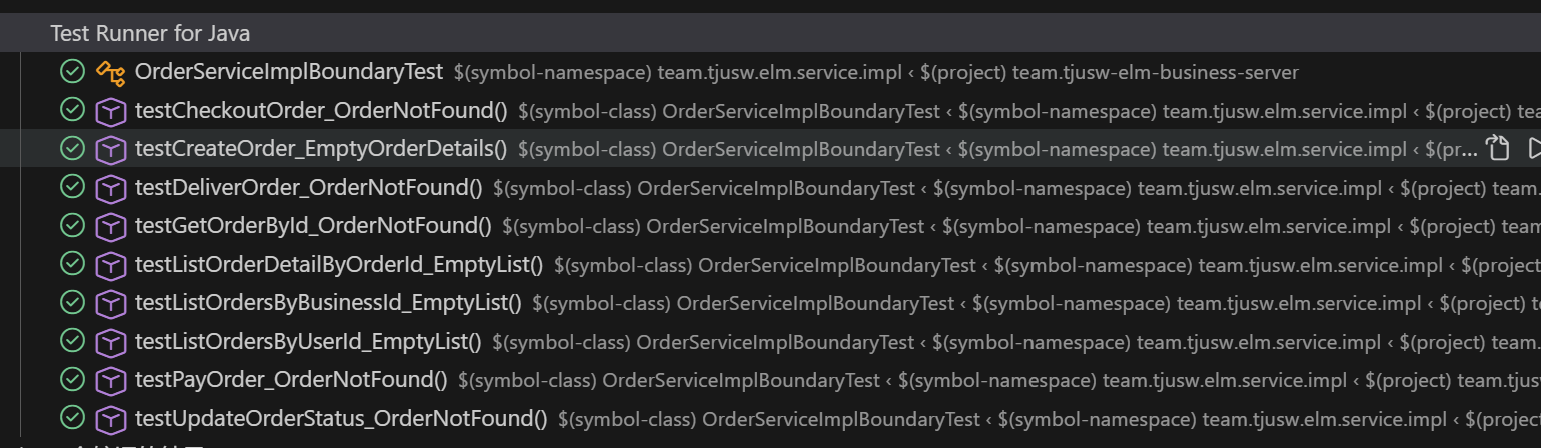
\includegraphics[width=0.85\textwidth,height=0.82\textheight,keepaspectratio]{images/test-order-service-result.png}
	\caption{订单服务OrdersService集成测试结果}
	\label{fig:test-orders-service}
\end{figure}

\section{配送地址微服务测试 (elm-delivery-server)}

\subsection{测试设计}

配送地址模块包含2个SpringBootTest集成测试类：

\textbf{DeliveryAddressControllerTest}（3个用例）：测试查询用户地址列表（验证返回1条记录）、查询单个地址（验证userId一致）、新增地址（期望201和返回1）。

\textbf{DeliveryAddressServiceTest}（4个用例）：测试查询地址列表、新增地址后列表增长、更新地址——验证旧地址失效（valid=0）且新增一条新地址、删除地址——验证valid变为0且有效列表为空。

\subsection{测试结果}

\begin{figure}[H]
	\centering
	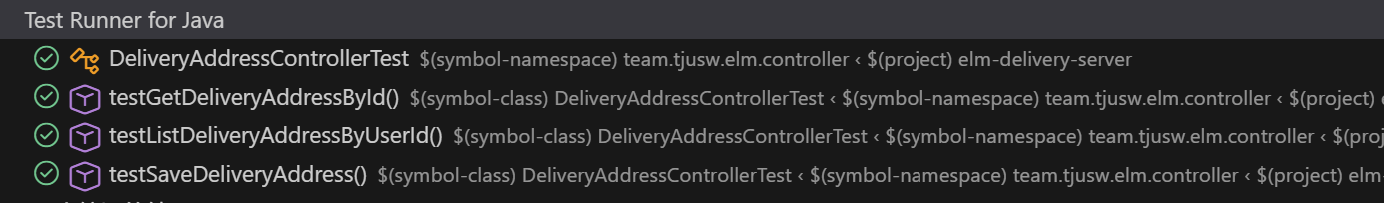
\includegraphics[width=0.85\textwidth,height=0.82\textheight,keepaspectratio]{images/test-delivery-controller-result.png}
	\caption{配送地址Controller测试结果}
	\label{fig:test-delivery-controller}
\end{figure}

\begin{figure}[H]
	\centering
	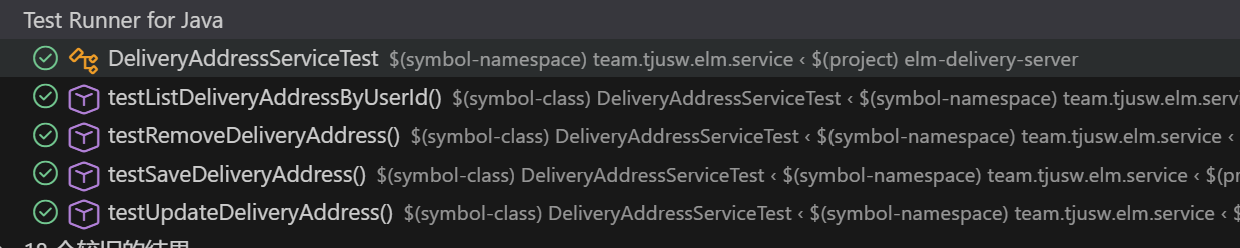
\includegraphics[width=0.85\textwidth,height=0.82\textheight,keepaspectratio]{images/test-delivery-service-result.png}
	\caption{配送地址Service集成测试结果}
	\label{fig:test-delivery-service}
\end{figure}

\section{虚拟钱包微服务测试 (elm-wallet-server)}

\subsection{测试设计}

钱包模块包含2个测试类：

\textbf{VirtualWalletControllerTest}（2个用例）：Mock HttpServletRequest和VirtualWalletService，测试从JWT Token中解析userId并查询钱包余额。使用Base64编码构造无签名JWT（\verb|\{"alg":"none"\}|），验证Controller正确委托Service并返回200和正确userId。

\textbf{VirtualWalletServiceImplTest}（1个用例）：Mock VirtualWalletMapper，测试getBalance方法查询余额（期望返回100.00）。

\subsection{测试结果}

\begin{figure}[H]
	\centering
	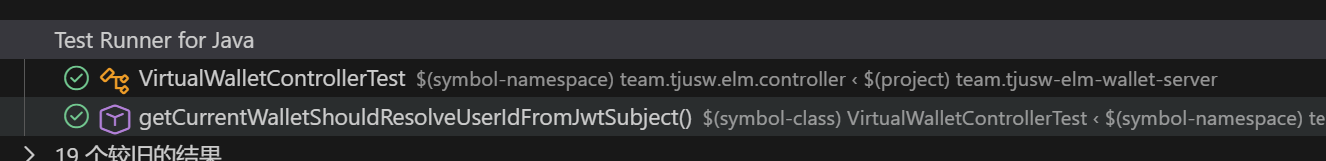
\includegraphics[width=0.85\textwidth,height=0.82\textheight,keepaspectratio]{images/test-wallet-controller-result.png}
	\caption{虚拟钱包Controller测试结果}
	\label{fig:test-wallet-controller}
\end{figure}

\begin{figure}[H]
	\centering
	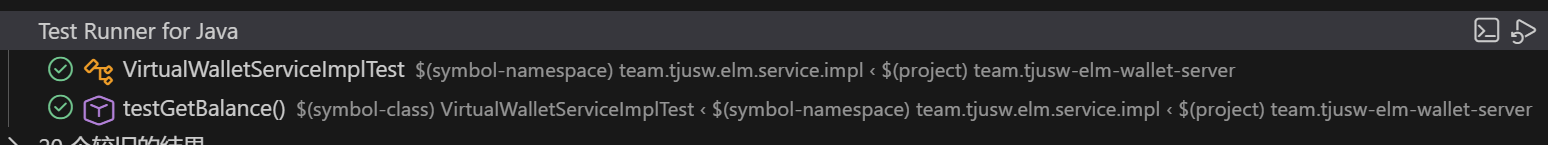
\includegraphics[width=0.85\textwidth,height=0.82\textheight,keepaspectratio]{images/test-wallet-service-result.png}
	\caption{虚拟钱包Service测试结果}
	\label{fig:test-wallet-service}
\end{figure}

\section{积分微服务测试 (elm-point-server)}

\subsection{测试设计}

积分模块是测试覆盖最全面的模块，包含4个测试类：

\textbf{IntegralMapperTest}（7个用例）：\verb|@SpringBootTest|测试真实数据库操作：插入积分记录并验证自增ID、按ID查询、按用户ID时间倒序查询、按状态和过期时间正向排序查询、更新积分状态和剩余数量、按用户和状态汇总可用积分、多用户数据隔离验证。

\textbf{IntegralServiceTest}（17个用例）：测试核心业务逻辑——增加积分、消费积分（成功/积分不足异常）、获取可用积分、首次签到（验证10积分和签到标记）、签到重复（返回0）、订单金额积分计算（取整规则）、评论积分计算（15字阈值，无图5分/有图10分）、积分抵扣计算（100积分=1元，最多抵扣订单金额）、积分明细查询、积分统计（总计/可用/已用/过期）、VIP积分（BASIC/GOLD/PLATINUM/DIAMOND）、活动积分（NEW\_USER/HOLIDAY/UNKNOWN）、生日积分（当天100分/当月10分/非当月0分）、连续签到积分（1-6天1分/7天10分/30天50分）、积分渠道验证、积分过期处理、可用积分详情。

\textbf{IntegralControllerTest}（13个用例）：\verb|@SpringBootTest|测试REST API接口——获取可用积分、手动添加积分、消费积分成功、首次签到、重复签到、评论积分（不满足条件/满足条件无图/满足条件有图）、积分抵扣计算、积分统计、订单发放积分、可用积分详情、积分渠道验证、积分过期处理。

\textbf{PointServiceImplTest}（4个用例）：Mock IntegralService和OrderClient，测试PointService作为Feign代理层正确转发调用——String类型userId的getBalance、earnPointByOrder、deductOrder，以及遗留数字文本userId。

\subsection{测试结果}

\begin{figure}[H]
	\centering
	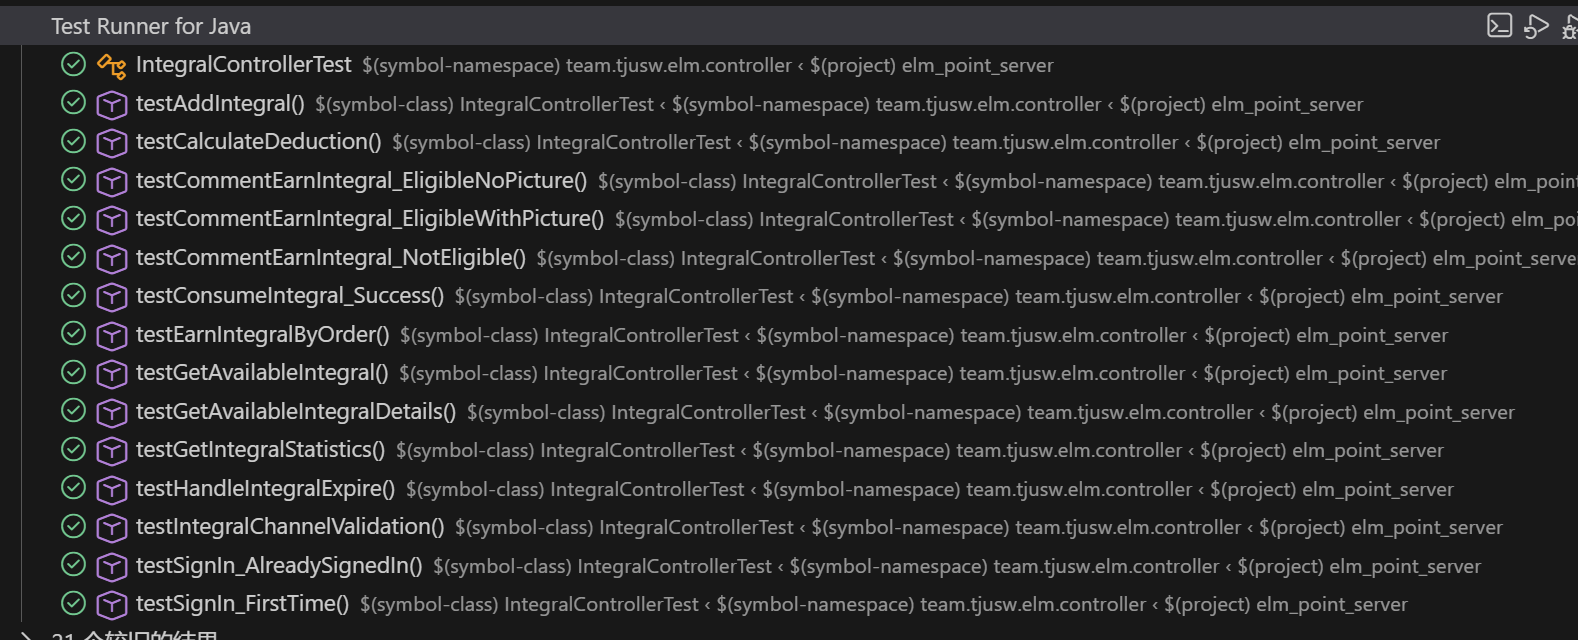
\includegraphics[width=0.85\textwidth,height=0.82\textheight,keepaspectratio]{images/test-integral-controller-result.png}
	\caption{积分Controller测试结果}
	\label{fig:test-integral-controller}
\end{figure}

\begin{figure}[H]
	\centering
	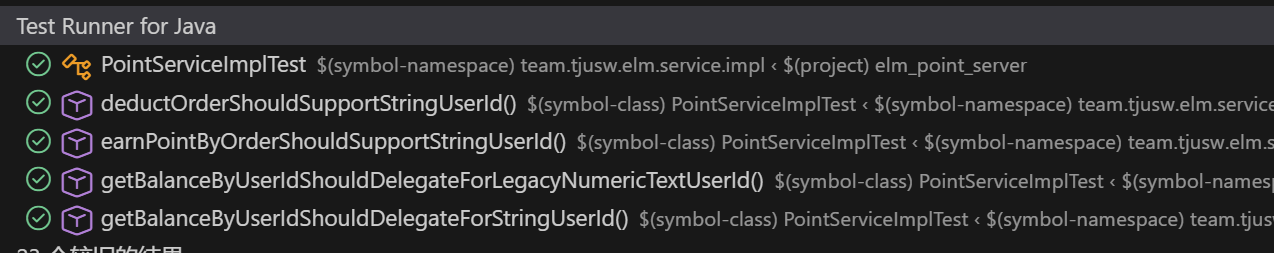
\includegraphics[width=0.85\textwidth,height=0.82\textheight,keepaspectratio]{images/test-integral-service-result.png}
	\caption{积分Service业务逻辑测试结果}
	\label{fig:test-integral-service}
\end{figure}

\begin{figure}[H]
	\centering
	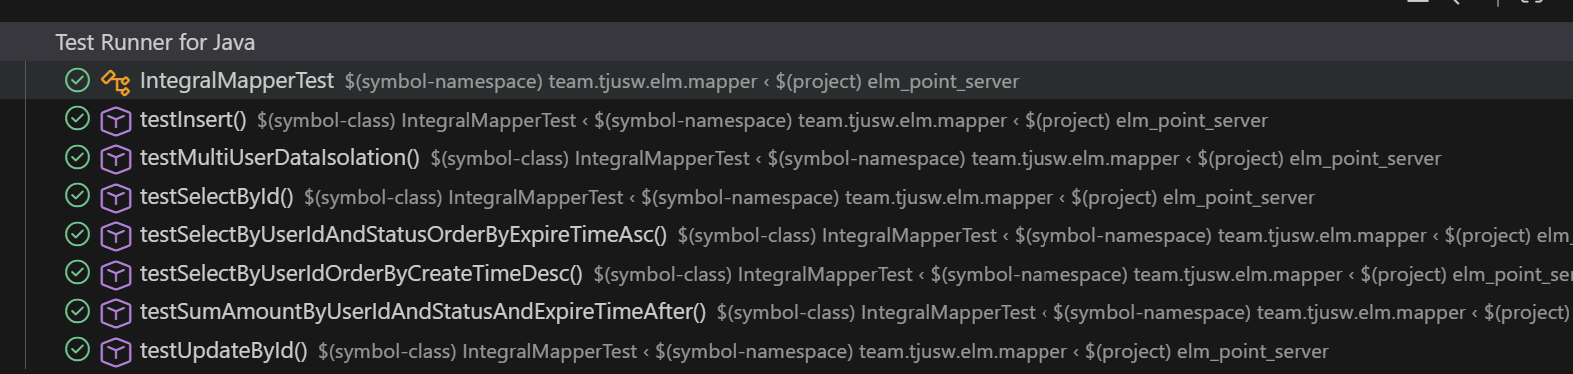
\includegraphics[width=0.85\textwidth,height=0.82\textheight,keepaspectratio]{images/test-integral-mapper-result.png}
	\caption{积分Mapper数据访问层测试结果}
	\label{fig:test-integral-mapper}
\end{figure}

\begin{figure}[H]
	\centering
	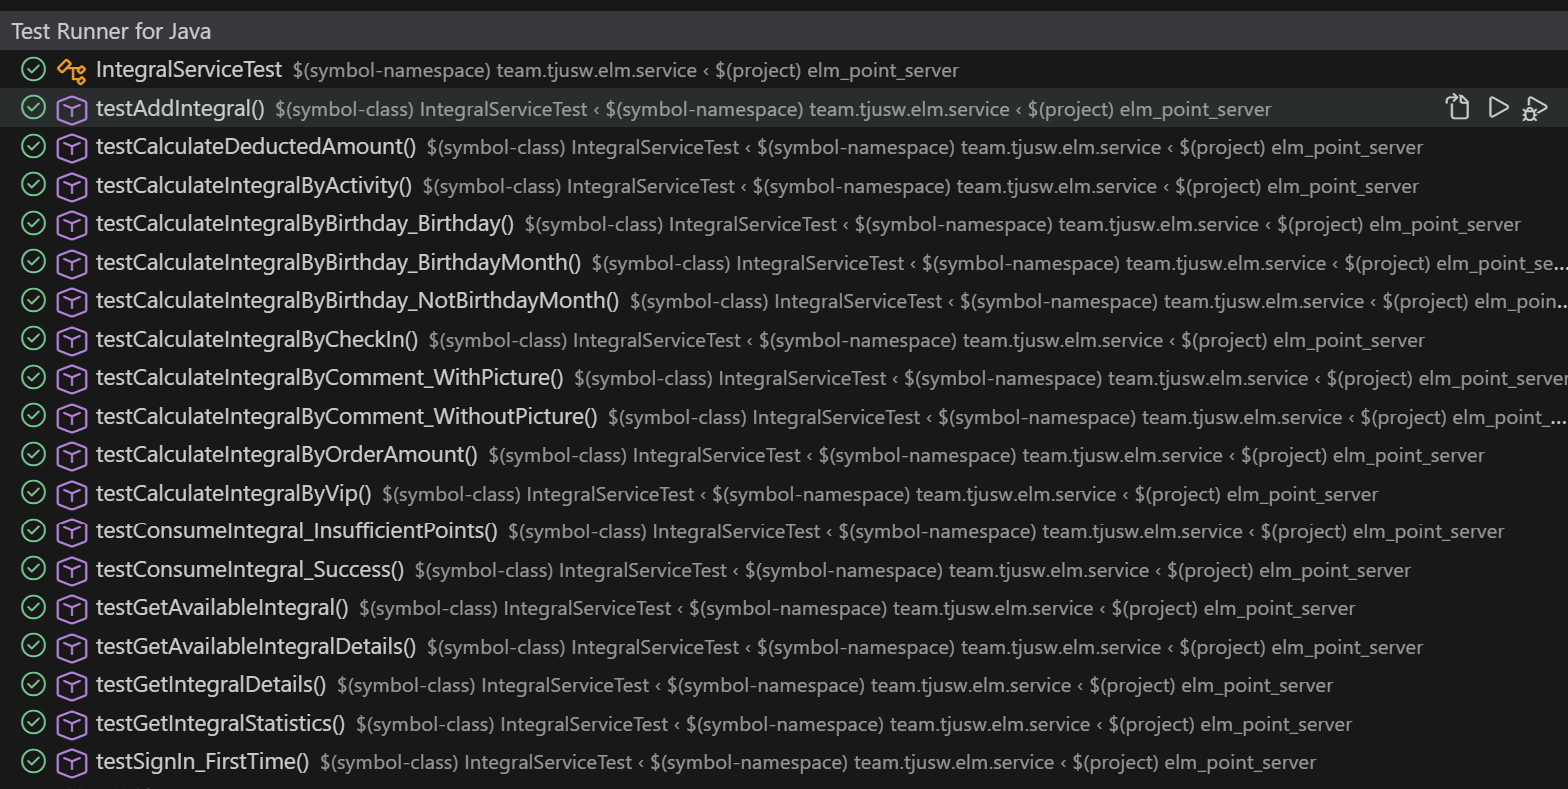
\includegraphics[width=0.85\textwidth,height=0.82\textheight,keepaspectratio]{images/test-point-service-result.png}
	\caption{PointService Feign代理测试结果}
	\label{fig:test-point-service}
\end{figure}

\section{测试覆盖汇总}

\begin{table}[H]
	\centering
	\caption{测试覆盖矩阵}
	\begin{tabular}{p{4.5cm}p{2.5cm}p{2.5cm}p{2.5cm}p{2.5cm}}
		\hline
		\textbf{模块} & \textbf{Controller} & \textbf{Service} & \textbf{Mapper} & \textbf{Boundary} \\
		\hline
		elm-user-server & $\checkmark$ & -- & -- & -- \\
		elm-business-server & $\checkmark$ & $\checkmark$ & -- & $\checkmark$ \\
		elm-food-server & $\checkmark$ & -- & -- & -- \\
		elm-cart-server & $\checkmark$ & $\checkmark$ & -- & $\checkmark$ \\
		elm-order-server & $\checkmark$ & $\checkmark$ & -- & -- \\
		elm-delivery-server & $\checkmark$ & $\checkmark$ & -- & -- \\
		elm-wallet-server & $\checkmark$ & $\checkmark$ & -- & -- \\
		elm-point-server & $\checkmark$ & $\checkmark$ & $\checkmark$ & -- \\
		\hline
	\end{tabular}
\end{table}

\section{测试设计要点}

\subsection{两种测试模式的选用}

项目使用两种Spring测试模式：

\begin{itemize}
	\item \textbf{MockMvc独立模式}（11个测试类）：\verb|MockMvcBuilders.standaloneSetup(controller).build()|，不加载Spring上下文，启动极快。适用于Controller层REST接口验证——只需Mock Service层，验证HTTP状态码、JSON响应结构和错误码语义
	\item \textbf{Spring Boot集成模式}（8个测试类）：\verb|@SpringBootTest| + \verb|@Transactional|，加载完整Spring上下文和真实数据库。使用\verb|@MockBean|仅替换Feign客户端（跨服务调用），保留真实Service和Mapper，验证业务逻辑完整链路
\end{itemize}

\subsection{交易完整性测试}

订单支付测试是重点验证对象：

\begin{itemize}
	\item \textbf{正常支付链路}：Mock完整Feign调用链——获取商家信息→查询余额→查询积分→计算积分抵扣→执行转账→发放消费积分→扣除订单积分，验证每步调用均发生且订单状态正确变更为1
	\item \textbf{余额不足}：设置钱包余额为10元、订单需支付23元（含1元积分抵扣），验证返回错误码，确保未执行转账
	\item \textbf{重复支付（幂等性）}：第一次支付成功返回200，第二次对同一订单支付返回409和状态码3，验证幂等性保护
\end{itemize}

\subsection{边界条件测试}

3个BoundaryTest类系统化覆盖以下边界场景：

\begin{itemize}
	\item 空列表输入（如空订单详情创建订单，期望总金额为0.0且不调用saveOrderDetail）
	\item null返回值（如查询不存在的订单返回null，期望不触发后续MQ消息发送）
	\item 零值输入（如购物车数量为零，期望正常处理）
	\item 不存在的数据操作（如更新不存在的订单返回0）
	\item 重复操作（如重复签到返回0积分、重复支付被拒绝）
	\item 数据隔离（如多用户积分数据互不影响）
\end{itemize}
   % 测试设计与结果
	% !Mode:: "TeX:UTF-8"

\chapter{总结}

\section{技术栈总结}

本项目实现了一个基于Spring Cloud微服务架构的外卖点餐平台，完整覆盖了从用户注册、商家浏览、点餐下单到钱包支付、积分管理的全业务流程。项目在以下方面体现了微服务架构的核心能力：

\begin{enumerate}
	\item \textbf{服务治理}：通过Eureka实现服务注册发现，支持Peer-to-Peer集群高可用，心跳续约间隔5秒，租约过期15秒
	\item \textbf{负载均衡}：通过Spring Cloud LoadBalancer实现客户端负载均衡，Gateway路由使用lb://前缀，Feign内置负载均衡，Eager Load消除冷启动延迟
	\item \textbf{声明式调用}：通过9个Feign客户端简化微服务间通信，集成Fallback降级逻辑，严格遵循单向无循环依赖
	\item \textbf{容错降级}：通过Resilience4j在Gateway层为9个服务配置独立熔断器（20秒超时），FallbackController返回包含fallback/retryable/service元数据的降级响应；Feign层集成Fallback实现兜底数据返回
	\item \textbf{API网关}：通过Spring Cloud Gateway实现统一入口，15条路由规则覆盖所有微服务，自定义缓存过滤器将重复GET请求从秒级降至毫秒级
	\item \textbf{配置管理}：通过Spring Cloud Config（native模式）实现集中配置，参数化配置支持环境变量覆盖；通过Spring Cloud Bus + RabbitMQ实现配置动态刷新
	\item \textbf{数据一致性}：通过Redisson分布式锁（锁超时10秒）保障金钱交易的一致性；通过Spring @Transactional保障订单创建与购物车清空的原子性
	\item \textbf{异步解耦}：通过RabbitMQ（DirectExchange + 明确路由键）实现订单状态异步通知，降低商家服务与购物车服务之间的耦合
\end{enumerate}

\section{通信方式对比}

\begin{table}[H]
	\centering
	\caption{服务间通信方式对比}
	\begin{tabular}{p{4.0cm}p{5.0cm}p{5.0cm}}
		\hline
		\textbf{对比维度} & \textbf{Feign同步调用} & \textbf{RabbitMQ异步消息} \\
		\hline
		应用场景 & 订单创建、支付（需即时响应） & 订单状态变更通知 \\
		耦合度 & 调用方依赖被调用方接口 & 生产者和消费者完全解耦 \\
		可靠性 & 调用失败即失败（有Fallback） & 消息持久化，支持重试 \\
		实时性 & 同步等待响应 & 异步处理，延迟低 \\
		\hline
	\end{tabular}
\end{table}

\section{容错机制分层}

Gateway层熔断（Resilience4j，Timeout=20s）保障外部请求的可用性，返回包含fallback元数据的降级响应（HTTP 403）；Feign层降级（Fallback实现类）保障内部服务间调用的鲁棒性，返回模拟的兜底数据。两层容错互为补充，形成纵深防御体系。

\section{RESTful API设计原则}

本项目严格遵循RESTful规范：将数据库表项映射为"资源"，URL表示资源路径；使用HTTP方法语义（GET/POST/PUT/DELETE）；资源路径使用复数名词；通过路径参数表达资源层级；统一使用CommonResult(code, message, result)响应格式。团队编写了《RESTful API接口规格说明书》，前后端基于文档并行开发。

\section{业务对象设计优化}

金额类型全部使用BigDecimal，避免浮点数精度问题；对象关联通过主键引用（Order存储businessId而非Business对象），将订单响应大小从MB级降至KB级，显著降低了微服务耦合度。

\section{测试设计总结}

项目编写了19个测试类共131个测试用例，覆盖全部8个微服务模块。测试采用四层金字塔架构：Mapper层（真实数据库+事务回滚）、Service层（Mockito单元测试）、Controller层（MockMvc独立模式）、边界条件层（空值/零值/重复操作/数据隔离）。点餐订单支付链路为测试重点，通过MockBean模拟完整Feign调用链验证交易完整性、余额不足拒绝和重复支付幂等性。

\section{小组成员分工}

\begin{table}[H]
	\centering
	\caption{小组成员分工}
	\begin{tabular}{p{2.8cm}p{11.5cm}}
		\hline
		\textbf{成员} & \textbf{负责内容} \\
		\hline
		杨博 & 测试设计与实现、point积分微服务开发、熔断降级前后端调试、前后端联调 \\
		\hline
		任晓华 & food食品微服务开发、wallet钱包微服务开发、对应功能模块测试 \\
		\hline
		陈宇泽 & delivery配送地址微服务开发、order订单微服务开发、对应功能模块测试 \\
		\hline
		魏语菲 & cart购物车微服务开发、business商家微服务开发、对应功能模块测试 \\
		\hline
		牛文航 & 数据库设计与搭建、user用户微服务开发、前后端联调 \\
		\hline
	\end{tabular}
\end{table}

\section{项目展望}

项目在功能覆盖上完成了核心业务闭环与扩展能力展示，后续可在以下方向改进：完善密码哈希与密钥管理等安全基线；引入自动化接口测试与端到端回归用例；扩充网关缓存淘汰机制（如LRU）；引入更完善的监控与告警体系；持续提高测试覆盖率，特别是Service层单元测试的覆盖广度。
   % 总结
	% \clearpage

\def\atemp{pdflatex}\ifx\atemp\usewhat
\end{CJK*}                                     % 结束中文字体使用（仅 pdflatex 模式）
\fi
\end{document}                                 % 结束全文
